%
%   Prof. Dr. Julian Reichwald
%   auf Basis einer Vorlage von Prof. Dr. Jörg Baumgart
%   DHBW Mannheim
%
%
%	ACHTUNG: Für das Erstellen des Literaturverzeichnisses wird das modernere Paket biblatex
%			 in Kombination mit biber verwendet -- nicht mehr das ältere BibTex!
% 			 Bitte stellen Sie ggf. Ihre TeX-Umgebung
% 			 entsprechend ein (z.B. TeXStudio: Einstellungen --> Erzeugen --> Standard Bibliographieprogramm: biber)
%

\documentclass[
	12pt,
	BCOR=5mm,
	DIV=12,
	headinclude=on,
	footinclude=off,
	parskip=half,
	bibliography=totoc,
	listof=entryprefix,
	toc=listof,
	pointlessnumbers,
	plainfootsepline,
	headings=optiontohead]{scrreprt}


%	Konfigurationsdatei einziehen
% !TEX root =  master.tex

%		LANGUAGE SETTINGS AND FONT ENCODING 
%
\usepackage[ngerman]{babel} 	% German language
\usepackage[utf8]{inputenc}
\usepackage{eurosym} % Euro symbol 
\usepackage[german=quotes]{csquotes} 	% correct quotes using \enquote{}
\usepackage[T1]{fontenc}
\usepackage{amssymb} % Mathe-Package
\usepackage{pdfpages} % for appendix pdfs


%\usepackage[english]{babel}   % For english language
%\usepackage{csquotes} 	% Richtiges Setzen der Anführungszeichen mit \enquote{}

% 		HYPERREF
%
\usepackage[
	hidelinks=true % keine roten Markierungen bei Links
]{hyperref}

% Zwei eigene Befehle zum Setzen von Autor und Titel. Ausserdem werden die PDF-Informationen richtig gesetzt.
\newcommand{\TitelDerArbeit}[1]{\def\DerTitelDerArbeit{#1}\hypersetup{pdftitle={#1}}}
\newcommand{\AutorDerArbeit}[1]{\def\DerAutorDerArbeit{#1}\hypersetup{pdfauthor={#1}}}
\newcommand{\Firma}[1]{\def\DerNameDerFirma{#1}}
\newcommand{\Kurs}[1]{\def\DieKursbezeichnung{#1}}


% Correct superscripts 
\usepackage{fnpct}


%		CALCULATIONS
%
\usepackage{calc} % Used for extra space below footsepline



%		BIBLIOGRAPHY SETTINGS
%

% Uncomment the next three lines for author-year-style with footnotes (Chicago)
\usepackage[backend=biber, autocite=footnote, style=authoryear, dashed=false]{biblatex} 	%Use Author-Year-Cites with footnotes
\AdaptNoteOpt\footcite\multfootcite   %will add  separators if footcite is called multiple consecutive times 
\AdaptNoteOpt\autocite\multautocite % will add  separators if autocite is called multiple consecutive times

% Uncomment the next line for IEEE-style 
% \usepackage[backend=biber, autocite=inline, style=ieee]{biblatex} 	% Use IEEE-Style (e.g. [1])

% Uncomment the next line for alphabetic style 
% \usepackage[backend=biber, autocite=inline, style=alphabetic]{biblatex} 	% Use alphabetic style (e.g. [TGK12])

% Uncomment the next two lines vor Harvard-Style 
%\usepackage[backend=biber, style=apa]{biblatex} 	
%\DeclareLanguageMapping{german}{german-apa}


\DefineBibliographyStrings{ngerman}{  %Change u.a. to et al. (german only!)
	andothers = {{et\,al\adddot}},
}

%%% Uncomment the following lines to support hard URL breaks in bibliography 
%\apptocmd{\UrlBreaks}{\do\f\do\m}{}{}
%\setcounter{biburllcpenalty}{9000}% Kleinbuchstaben
%\setcounter{biburlucpenalty}{9000}% Großbuchstaben


\setlength{\bibparsep}{\parskip}		%add some space between biblatex entries in the bibliography
\addbibresource{bibliography.bib}	%Add file bibliography.bib as biblatex resource


%		FOOTNOTES 
%
% Count footnotes over chapters
\usepackage{chngcntr}
\counterwithout{footnote}{chapter}

%	ACRONYMS
%%%
%%% WICHTIG: Installieren Sie das neueste Acronyms-Paket!!!
%%%
\makeatletter
\usepackage[printonlyused]{acronym}
\@ifpackagelater{acronym}{2015/03/20}
  {%
    \renewcommand*{\aclabelfont}[1]{\textbf{\textsf{\acsfont{#1}}}}
  }%
  {%
  }%
\makeatother

%		LISTINGS
\usepackage{listings}	%Format Listings properly
\renewcommand{\lstlistingname}{Quelltext}
\renewcommand{\lstlistlistingname}{Quelltextverzeichnis}
\lstset{numbers=left,
	numberstyle=\tiny,
	captionpos=b,
	basicstyle=\ttfamily\small,
	commentstyle=\itshape,
	breaklines=true, 
	breakatwhitespace=true,
	showstringspaces=false,
	escapeinside={@@},
	keywordstyle=\bfseries,
	postbreak=\raisebox{0ex}[0ex][0ex]{\ensuremath{\hookrightarrow\space}}
	}

%LISTING inline a tabular/table
\newcommand\tablstinline[2][]{\lstinline[#1]{#2}}

% LISTINGS: eigene Programmiersprache; bei morekeywords die zusätzlichen einfügen
\lstdefinelanguage{PLSQL}{
	language     = SQL,
	morekeywords = {over, partition}}

% ---- LISTING FOR YAML FILES ----
%\usepackage[dvipsnames]{xcolor}
%\usepackage{listings}
\usepackage{color}
\newcommand\YAMLcolonstyle{\color{red}\mdseries}
\newcommand\YAMLkeystyle{\color{black}\bfseries}
\newcommand\YAMLvaluestyle{\color{black}\mdseries}

\makeatletter

% here is a macro expanding to the name of the language
% (handy if you decide to change it further down the road)
\newcommand\language@yaml{yaml}

\expandafter\expandafter\expandafter\lstdefinelanguage
\expandafter{\language@yaml}
{
	keywords={true,false,null,y,n},
	keywordstyle=\color{darkgray}\bfseries,
	basicstyle=\YAMLkeystyle,                                 % assuming a key comes first
	sensitive=false,
	comment=[l]{\#},
	morecomment=[s]{/*}{*/},
	commentstyle=\color{purple}\ttfamily,
	stringstyle=\YAMLvaluestyle\ttfamily,
	moredelim=[l][\color{orange}]{\&},
	moredelim=[l][\color{magenta}]{*},
	moredelim=**[il][\YAMLcolonstyle{:}\YAMLvaluestyle]{:},   % switch to value style at :
	morestring=[b]',
	morestring=[b]",
	literate =    {---}{{\ProcessThreeDashes}}3
	{>}{{\textcolor{red}\textgreater}}1     
	{|}{{\textcolor{red}\textbar}}1 
	{\ -\ }{{\mdseries\ -\ }}3,
}

% switch to key style at EOL
\lst@AddToHook{EveryLine}{\ifx\lst@language\language@yaml\YAMLkeystyle\fi}
\makeatother

\newcommand\ProcessThreeDashes{\llap{\color{cyan}\mdseries-{-}-}}
% --------------------------

%		EXTRA PACKAGES
\usepackage{lipsum}    %Blindtext
\usepackage{graphicx} % use various graphics formats
\usepackage[german]{varioref} 	% nicer references \vref
\usepackage{caption}	%better Captions
\usepackage{booktabs} %nicer Tabs
\newcommand{\ra}[1]{\renewcommand{\arraystretch}{#1}}
\usepackage{longtable} %multipages booktabs
\usepackage{array}
%\newcolumntype{P}[1]{>{\raggedright\arraybackslash}p{#1}}


%		ALGORITHMS
\usepackage{algorithm} %float wrapper for algorithms.
\usepackage{algpseudocode}
\renewcommand{\listalgorithmname}{Algorithmenverzeichnis }
\floatname{algorithm}{Algorithmus}


%		FONT SELECTION: Entweder Latin Modern oder Times / Helvetica
\usepackage{lmodern} %Latin modern font
%\usepackage{mathptmx}  %Helvetica / Times New Roman fonts (2 lines)
%\usepackage[scaled=.92]{helvet} %Helvetica / Times New Roman fonts (2 lines)

%		PAGE HEADER / FOOTER
%	    Warning: There are some redefinitions throughout the master.tex-file!  DON'T CHANGE THESE REDEFINITIONS!
\RequirePackage[automark,headsepline,footsepline]{scrpage2}
\pagestyle{scrheadings}
\renewcommand*{\pnumfont}{\upshape\sffamily}
\renewcommand*{\headfont}{\upshape\sffamily}
\renewcommand*{\footfont}{\upshape\sffamily}
\renewcommand{\chaptermarkformat}{}
\RedeclareSectionCommand[beforeskip=0pt]{chapter}
\clearscrheadfoot


\ifoot[\rule{0pt}{\ht\strutbox+\dp\strutbox}DHBW Mannheim]{\rule{0pt}{\ht\strutbox+\dp\strutbox}DHBW Mannheim}
\ofoot[\rule{0pt}{\ht\strutbox+\dp\strutbox}\pagemark]{\rule{0pt}{\ht\strutbox+\dp\strutbox}\pagemark}

\ohead{\headmark}


\begin{document}

%% BITTE GEBEN SIE HIER DEN TITEL UND DIE AUTORIN / DEN AUTOR DER ARBEIT AN!
%% DIESE INFORMATIONEN _MÜSSEN_ GESETZT SEIN, UM TITELBLATT, ABSTRACT UND
%% EIGENSTÄNDIGKEITSERKLÄRUNG AUTOMATISCH ANZUPASSEN!

\TitelDerArbeit{Integration einer Container-Umgebung in einen automatisierten Deployment-Prozess und die Untersuchung ihrer Effekte auf diesen}
\AutorDerArbeit{Yves Torsten Staudenmaier}
\Firma{SV Informatik GmbH}
\Kurs{WWI17SEC}

\begin{titlepage}
\begin{minipage}{\textwidth}
		\vspace{-2cm}
		\noindent 
\includegraphics[scale=0.67]{img/logoeps/SVI-logo-claim.eps} \hfill   
\includegraphics[scale=0.79]{img/logo.jpg}
\end{minipage}
\vspace{1em}
\sffamily
\begin{center}
	\textsf{\large{}Duale Hochschule Baden-W\"urttemberg\\[1.5mm] Mannheim}\\[2em]
	\textsf{\textbf{\Large{}Bachelorthesis}}\\[3mm]
	\textsf{\textbf{\DerTitelDerArbeit}} \\[1.5cm]
	\textsf{\textbf{\Large{}Studiengang Wirtschaftsinformatik}\\[3mm] \textsf{Studienrichtung Software Engineering}}
	
	\vspace{3em}
	\textsf{\Large{Sperrvermerk}}
\vfill

\begin{minipage}{\textwidth}

\begin{tabbing}
	Wissenschaftlicher Betreuer: \hspace{0.85cm}\=\kill
	Verfasser/in: \> \DerAutorDerArbeit \\[1.5mm]
	Matrikelnummer: \> 7146590 \\[1.5mm]
	Firma: \> \DerNameDerFirma  \\[1.5mm]
	Abteilung: \> IE2 -- Deployment \\[1.5mm]
	Kurs: \> \DieKursbezeichnung \\[1.5mm]
	Studiengangsleiter: \> Prof. Dr.-Ing. habil. Dennis Pfisterer \\[1.5mm]
	Wissenschaftlicher Betreuer: \> Marius Ebel \\
	\> info@mariusebel.net \\
	\> +49 176 / 473 45452 \\[1.5mm]
	Firmenbetreuer: \> Thomas Teske \\
	\> thomas.teske@sv-informatik.de \\
	\> +49 621 / 454 44096 \\[1.5mm]
	Lektorat: \> Rita Galli \\[1.5mm]
	Bearbeitungszeitraum: \> 17.02.---08.05.2020
\end{tabbing}
\end{minipage}

\end{center}

\end{titlepage}

\pagenumbering{Roman} % Römische Seitennummerierung
\normalfont

%--------------------------------
% Verzeichnisse - nicht benötige Verzeichnisse bitte auskommentieren / löschen.
%--------------------------------

%   Sperrvermerk
\chapter*{Sperrvermerk}
Der Inhalt dieser Arbeit darf weder als Ganzes noch in Auszügen Personen au"serhalb des Prüfungsprozesses und des Evaluationsverfahrens zugänglich gemacht werden, sofern keine anders lautende Genehmigung der Ausbildungsstätte vorliegt. Die Bachelorarbeit enthält unternehmensinterne Architektur- und Prozessmodellierungen und deren Dokumentation. Es ist zum Zeitpunkt der Anmeldung nicht sicher, ob interne Schnittstellen in der Anwendungslandschaft offengelegt werden.


\vspace{3cm}
\noindent Mannheim, 05.05.2020\hfill\rule{8.4cm}{.4pt}\par
\noindent\hfill Annalena Haus, Ausbildungsverantwortliche
\cleardoublepage



% Lesehinweis
\chapter*{Lesehinweise}
Die folgenden Hinweise sollen das Lesen dieser Projektarbeit erleichtern und spezielle Formatierung definieren:

\begin{itemize}
	\item Im Sinne der Gleichberechtigung wird in dieser Arbeit entweder die Form \textit{\enquote{die Entwickler*in}} oder die grammatikalisch korrekte Form \textit{\enquote{die/der Entwickler/-in}} verwendet werden. Bei der Kurzform mit der Sternnotation wird auf Grund der Lesbarkeit der weibliche Artikel benutzt.
	\item Abbildungen, die mit dem Vermerk \textit{unternehmensintern} gekennzeichnet sind, unterliegen folgendem rechtlichen Hinweis: \enquote{Alle Rechte, einschließlich der Vervielfältigung, Veröffentlichung, Bearbeitung und Übersetzung bleiben der SV Informatik GmbH vorbehalten.}
	\item Produkt- oder Eigennamen werden in \textsc{Kapitälchen} gesetzt, wie beispielsweise \textsc{Node.js}.
	\item Hochgestellte Ziffern weisen auf Fußnoten am Seitenende hin.
	
	
\end{itemize}
 

%	Kurzfassung
\chapter*{Kurzfassung}
\addcontentsline{toc}{chapter}{Abstract}
\begingroup
\begin{table}[h!]
\setlength\tabcolsep{0pt}
\begin{tabular}{p{3.7cm}p{11.7cm}}
Titel: & \DerTitelDerArbeit \\
Verfasser/-in: & \DerAutorDerArbeit \\
Kurs: & \DieKursbezeichnung \\
Ausbildungsstätte: & \DerNameDerFirma\\
\end{tabular}
\end{table}
\endgroup

%Überlege, ob ich den Header brauche mit den ganzen Infos? --> JA.
%Hier können Sie die Kurzfassung der Arbeit schreiben. 
Kurze Einleitung: Motivation, Einführung in den Themenkomplex, allgemeine Methodik
\par
Forschungsfrage eins: Frage + kurze Erläuterung - Methodik - Teil-Ergebnis
\par
Forschungsfrage zwei: Frage + kurze Erläuterung- Methodik - Teil-Ergebnis
\par
Forschungsfrage drei: Frage + kurze Erläuterung - Methodik - Teil-Ergebnis
\par
Minimalergebnis

%	Inhaltsverzeichnis
\tableofcontents

%	Abbildungsverzeichnis
\listoffigures 

%	Tabellenverzeichnis
\listoftables

%	Listingsverzeichnis
\lstlistoflistings
 

% 	Algorithmenverzeichnis
\listofalgorithms

% 	Abkürzungsverzeichnis (siehe Datei acronyms.tex!)
\clearpage
\chapter*{Abkürzungsverzeichnis}	
\addcontentsline{toc}{chapter}{Abkürzungsverzeichnis}


\begin{acronym}[RDBMS]
	\acro{AWL}{Anwendungslandschaft}
	\acro{DHBW}{Dualen Hochschule Baden-Württemberg}
	\acro{BaFin}{Bundesanstalt für Finanzdienstleistungsaufsicht}
	\acro{IE2}{IE2 -- Deployment}
	\acro{IE}{IE -- Entwicklungs- und Betriebsunterstützung}
	\acro{CAB}{\enquote{Change Advisory Board}}
	\acro{ITIL}{Information Technology Infrastructure Library}
	\acro{SV}{SV SparkassenVersicherung}
	\acro{SVI}{SV Informatik GmbH}
	\acro{SVS}{SV Sachsen}

\end{acronym}

\ohead{Acronyms} % Neue Header-Definition

%--------------------------------
% Start des Textteils der Arbeit
%--------------------------------
\clearpage
\ihead{\chaptername~\thechapter} % Neue Header-Definition (inner header)
\ohead{\headmark} % Neue Header-Definition (outer header)
\pagenumbering{arabic}  % Arabische Seitenzahlen

%	Anleitungs-Datei anleitung.tex einziehen. Auf diese Weise sollten Sie versuchen, für jedes einzelne
% Kapitel eine eigene Datei anzulegen und mittels input-Kommando einzuziehen.
%\input{anleitung}

%-----------------
% Kapitel einbinden
%-----------------

% reset memory of all acronyms, so \ac will print out full name of acronym!
\acresetall 
\hyphenation{An-wendungs-land-schaft} % because ngerman/babel doesn´t know it correctly... 

\chapter{Einleitung}\label{kap:einleitung}
\paragraph{Motivation der Arbeit}
Die \ac{SV} ist bestrebt ihre Versicherungsprozesse und den Kontakt mit den Kunden durch digitale Kanäle ständig zu verbessern. Die Digitalisierung ist ein wichtiger Bestandteil der \ac{SV}-Strategie: So ist sie Mitbegründerin der \enquote{id-fabrik}\footnote{Ein Start-up, das federführend Innovationen im Bereich der S-Finanzgruppe erzeugt.} und Mitglied im \enquote{InsurLab Germany}\autocite[vgl.][S.\,30]{sv_sparkassenversicherung_sv_2019}. Um die Anforderungen der \ac{SV}-Kunden nach ständiger Verfügbarkeit und hoher Servicequalität zu erfüllen, muss die \ac{SV} ihre \ac{AWL} ständig an diese Anforderungen anpassen. Die Nachfrage der \ac{SV}-Kunden und damit die daraus resultierenden Anforderungen an die Systeme, stellt die IT-Dienstleisterin (\ac{SVI}) der \ac{SV} vor neue Herausforderungen. Die Verteilungsprozesse von neuen Versionen der Anwendungen können derzeit nicht während des laufenden Betriebes durchgeführt werden. So müssen neue Funktionen warten, bis das Wochenende des \enquote{Release} sie veröffentlicht, d.\,h. die \ac{TTM} der neuen Produkte ist sehr hoch. Diese Verzögerung der Produktveröffentlichung passt nicht zu der digitalen Strategiezielen der \ac{SV}. Als Lösungsansatz sind die Eigenschaften der \enquote{Cloud}-Technologie zu nennen. Jedoch muss aus IT-Sicht hier eine Anmerkung gemacht werden:

\begin{figure}[h!]
	\centering
	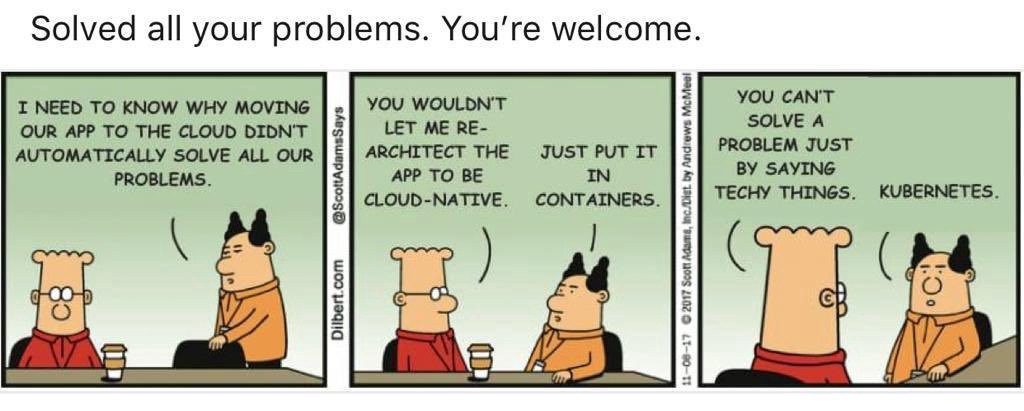
\includegraphics[scale=0.33]{img/dilbertCloud.jpeg}
	\caption{Dilbert-Comic zu \textsc{Kubernetes}}
	\label{abb:dilbertK8s}
	{\footnotesize Quelle: \cite{DilbertKubernetes}\par}
	{\footnotesize Redaktionelle Anmerkung: Abbildung nur als komprimiertes Format verfügbar (Qualitätseinbuße)}
\end{figure}

Die, in Abbildung \vref{abb:dilbertK8s}, dargestellte Aussage ist absichtlich überspitzt, um das Verständnis der Lösungsmöglichkeiten der \enquote{Cloud}-Technologie zu schärfen. Der Hinweis der IT stellt klar, dass das oben beschriebene Problem nur mit einer ganzheitlichen Lösung zu erreichen ist. Es führt nicht zum gewünschten Ergebnis, Anwendungen, die nicht für die \enquote{Cloud} gedacht sind, mit Zwang in diese zu bewegen. Diese Arbeit beschreibt den Prozess zur Verteilung von Container-Anwendungen. 

\paragraph{Problemstellung und -abgrenzung}
Bei der vorliegenden Arbeit handelt es sich um eine mehrteilige Analyse und Konzeption, die bei abgeschlossener Untersuchung ein Konzept zur automatischen Verteilung von Container-Anwendungen, die Betrachtung der Effekte von diesen Anwendungen und ein Ergebnis zu den sicherheitsrelevanten Aspekten dieses Prozess enthalten wird. Dabei akkumuliert sich der Fokus die Prozessentwicklung der Verteilung einer Container-Anwendung. Des Weiteren ist die Untersuchung der Anforderungen, die Analyse der \enquote{Cloud}-Plattform \textsc{OpenShift}\footnote{\enquote{\textsc{OpenShift} is an open source container application platform by Red Hat based on the Kubernetes container orchestrator for enterprise app development and deployment.} Quelle: \cite[][]{red_hat_inc_openshift_2020}} und die Erstellung eines Generierungsalgorithmus im Fokus dieser Arbeit. Dieser Teilkomplex wird durch die Forschungsfrage eins -- Wie können Container-Anwendungen den Prozess des automatisierten \enquote{Deployments}\footnote{\enquote{Software deployment may be considered to be a process consisting of a number of inter-related activities including the release of software at the end of the development cycle; the configuration of the software, the installation of software into the execution environment, and the activation of the software. It also includes post installation activities including the monitoring, deactivation, updating, reconfiguration, adaptation, redeploying and undeploying of the software.} (\cite{dearle_software_2007})} unterstützen? -- abgedeckt. Der Anforderungskatalog soll in Zusammenarbeit mit dem Fachbereich erstellt werden, um die Akzeptanz der Anforderungen zu steigern und um die Validität dieser zu gewährleisten. Die Forschungsfragen zwei und drei (siehe dazu Paragraph \enquote{Forschungsfragen/-design}) analysieren den wirtschaftlichen und sicherheits-/rechtlich-relevanten Bereich des Themenkomplexes der Bachelorarbeit. Dabei bedient sich die Forschungsfrage zwei der Methodik des Geschäftsvorfalls (\enquote{Business Case}). Beide Forschungsfragen werden durch eine Analyse des Ist-Zustands eine initiale Konzeption ableiten. 
\par
Nicht Teil dieser Arbeit ist die unternehmensinterne Entscheidung über die Verantwortlichkeiten des zu entwickelnden Prozesses und die Erstellung einer unternehmensweiten Strategie zum Container-\enquote{Deployment}. Die Anpassung des unternehmensinternen Prozesses \enquote{Release} ist nicht Teil dieser Arbeit. Dieser übersteigt die Anforderungen, die an diese Bachelorarbeit gestellt werden. Auch genügt die rechtliche Betrachtung des Einkaufsprozess von Software nicht den juristischen Ansprüchen eines Gutachtens. Dies ist jedoch nicht Ziel der Arbeit. Die wirtschaftliche Betrachtung des Geschäftsvorfalls  \enquote{Container-Verteilung} dient als reine Veranschaulichung der Methodik und genügt nicht einer vollständigen Betrachtung, die die \ac{BWL} vorgibt. Der Fokus der Arbeit liegt auf der technischen Entwicklung eines Verteilungsprozesses.

\paragraph{Zielstellung der Arbeit}\label{kap:einleitung:Ziele}
Folgende \textit{SMART}\footnote{\enquote{SMART-Regel sind Formulierungshilfen, die eine einfache Methode zum Operationalisieren von Zielen und auch zur Überprüfung der Güte von Zielen darstellen.} Quelle: \cite[][S.69]{dechange_projektmanagement_2020}} formulierte Ziele sollen diese Bachelorthesis leiten, messbar machen und später als Anhaltspunkt zur Evaluierung des Erfolgs dienen:

\begin{enumerate}
	\item Entwicklung eines Verteilungsprozess für einfache Container-Anwendungen bis zum 27.April 2020. Einfach bedeutet hier, dass die Container-Struktur aus einer \enquote{Base Image}\footnote{siehe dazu Kapitel \vref{kap:container}}-Schicht und einer Logik-Schnitt (Eigenentwicklung) besteht.
	\item Der Prozess muss zu 98\,\% ohne Einwirkung von Menschen während des Verteilungsvorgangs funktionieren, d.\,h. er ist (annähernd) voll automatisiert. Dies muss bis zum Ende des Bearbeitungszeitraum der Arbeit (8.Mai 2020) umgesetzt werden.
	\item Die Generierung einer Konfigurationsdatei soll in 9 von 10 Verteilungen automatisch mit einem Skript durchgeführt werden. Umzusetzen ist dies bis zum 08.Mai 2020.
	\item Die Vorteile einer Container-Anwendung für die Verteilung dieser sollen erforscht werden. Akzeptiert ist dieses Ziel, sobald eine Auflistung und eine kritische Betrachtung der Ergebnisse beschrieben wurde. Umzusetzen bis zum Ende des Bearbeitungszeitraums. (Dieses Ziel ist nicht komplett \textit{SMART}-konform, da die zumindest die Messbarkeit ohne genannte Messgröße nicht nachvollziehbar ist.)
	\item Die wirtschaftliche Betrachtung muss sich anhand des Standes von Wissenschaft und Technik orientieren. Dazu werden gängige Regeln von \cite{herman_is_2009}, \cite{brugger_it_2009} u.\,Ä. benutzt. Diese Betrachtung muss bis zum Ende des Bearbeitungszeitraums durchgeführt werden. Die Messbarkeit wird durch die Einhaltung der oben genannten Regeln beschrieben.
	\item Die sicherheits-/rechtlich-relevanten Aspekte dieses Projektes sollen anhand der, für die Finanzdienstleitungs- und Versicherungsbranche, geltenden Vorschriften beleuchtet werden. Der Umfang dieser Beleuchtung beschränkt sich auf das Nötigste, d.\,h. es müssen nur die wichtigsten Regeln beschrieben werden. Dies ist bis zum Ende des Bearbeitungszeitraumes umzusetzen. Die Messbarkeit ist durch die sicherheits-/rechtlich-relevanten Vorschriften bestimmt.
\end{enumerate}

\paragraph{Forschungsfragen/-design}\label{ffs}
Die Forschungsfragen, mit der sich diese Bachelorarbeit beschäftigen wird, sind eine direkte Konsequenz aus der Zielstellung der Arbeit und aus den unternehmensinternen Anforderungen an eines möglichst vollständig automatisierten Prozesses. Dabei liegt der Fokus auf der Betrachtung beider Teildisziplinen der Wirtschaftsinformatik, nämlich der Informatik und der Wirtschaft -- jedoch wird der größere Teil dieser Arbeit einen informationstechnischen Fokus haben. Die folgende Aufzählung nennt die einzelnen Forschungsfragen, die im weiteren Verlauf ein gemeinsames Ergebnis erbringen werden. Dieses ist in Kapitel \vref{kritischeBetrachtung} dargestellt.
\begin{enumerate}
	\item Wie können Container-Anwendungen den Prozess des automatisierten \enquote{Deployments} unterstützen?
	\item Welche wirtschaftlichen Vorteile hat der Einsatz von Containern auf den Prozess des automatisierten \enquote{Deployments}?
	\item Welche besonderen sicherheitstechnischen Aspekte muss ein solcher Prozess im Bereich der Versicherung erfüllen?
\end{enumerate}
% TODO: Nachfolgende Absätze auf Richtigkeit prüfen
Die Forschungsfrage eins wird einen Ist-Zustand analysieren. Diese Analyse enthält eine Betrachtung des Prozesses und einen Anforderungskatalog der Entwicklungsabteilungen an den zu konzeptionierenden \enquote{Deployment}-Prozess für Container-Anwendungen. Danach wird ein Konzept eines Container-basierten automatisierten \enquote{Deployment}-Prozesses erstellt, das aus der Entwicklung dieses und einer Standardisierung der beteiligten Dateien besteht. Die Forschungsfrage eins schließt mit einem Teilergebnis ab. \par

Die Forschungsfrage zwei beschäftigt sich mit den wirtschaftlichen Vorteil eines Einsatzes der Container auf den Prozess des automatisierten \enquote{Deployment}-Prozesses. Dabei wird der bestehende Geschäftsprozess \enquote{Release} analysiert und ein Ist-Soll-Vergleich der Methodik des \enquote{Business case} mit der Umsetzung im Unternehmen durchgeführt. Ein Ausblick schließt die Forschungsfrage zwei ab. 
\par
Die Forschungsfrage drei identifiziert sicherheitsrelevante Anforderungen, die nicht nur die Anwendung selbst betreffen, sondern Auswirkung auf die komplette Anwendungslandschaft (\acs{AWL}) haben. Diese Anforderungen werden durch das \acl{BSI} und verschiedene \textsc{DIN/ISO}-Normen beeinflusst. Außerdem soll analysiert werden, wie bei der Beschaffung von \enquote{Open source}- bzw. \enquote{Closed source}-Anwendungen mögliche Schwachstellen identifiziert werden, die potenzielle Angriffsvektoren in der \ac{AWL} eröffnen würden, und wie mit diesen verfahren wird. Dabei soll versucht werden Rückschlüsse auf die Anwendung \textsc{OpenShift} von \textsc{Red Hat\footnote{\enquote{Red Hat ist der weltweit führende Anbieter von Open-Source-Lösungen, die auf verlässlichen und leistungsstarken Technologien in den Bereichen \enquote{Cloud}, Virtualisierung, Storage, Linux, Mobile und Middleware basieren. Darüber hinaus bieten wir Support-, Trainings- und Consulting-Services an, die mehrfach prämiert wurden.} Quelle: \cite[][]{red_hat_inc_red_2020}}} zu ziehen. Auch hier wird ein Teilergebnis diese Forschungsfrage abschließen


\paragraph{Einordnung der Abteilung in den Geschäftsprozess}
Die Abteilung \ac{IE2}, die aus Sicht des unternehmensinternen Organigramms der Organisationseinheit \ac{IE} angehört, befasst sich in erster Linie mit dem Transport (\enquote{Deployment}) von Software-Artefakten der einzelnen Software-Produkte der \ac{SVI}. Diese werden für die \ac{SV} entwickelt, betrieben und gewartet. Zu den zentralen Aufgaben der Abteilung gehören die Planung, die Durchführung und die Überwachung der \enquote{Build/Deployment}-Prozesse der verschiedenen Service-Umgebungen, die aus mehreren Server-Verbünden bestehen. Des Weiteren stellt \ac{IE2} die Einspielung von datenbank-relevanten Objekten sicher. Auch entwickelt sie die Bau- und Transportprozesse kontinuierlich weiter und passt diese an die sich ständig verändernden Anforderungen der Entwicklungsabteilungen an. Von zentraler Bedeutung sind die Planung und die Durchführung der Veröffentlichungen der neuen Versionen einer zu betreuenden Anwendung. Zu dieser Aufgabe gehören auch Aufbau und Bereitstellung der Systemtest-, Releasetest- und Produktionsumgebungen. Eine weitere zentrale Aufgabe ist das Umgebungsmanagement. Die Aufgaben dieses Teilbereichs befassen sich mit folgenden Inhalten: Planung von Aktivitäten in der Produktionsumgebung, der Planung und der Koordination der Infrastruktur und Notfall-\enquote{Fix} der Produktion und der allgemeinen \enquote{Patch}-Planung; Beratung zur Erweiterung, Koordination und Planung von verschiedenen Testumgebungen. Außerdem ist das Umgebungsmanagement Teil des \ac{CAB}, das ein Gremium nach der \enquote{Best practice} \ac{ITIL} darstellt. Dieses ist für die Freigabe von \enquote{Changes} verantwortlich und hat sowohl ständige, als auch der Situation angepasste Mitglieder. 

\paragraph{Aufbau der Arbeit}
In Kapitel \vref{ff1} wird die Forschungsfrage eins behandelt. Diese beschreibt grundlegende Aspekte der Anforderungsanalyse, des \acl{Cloud-C} und der Container(-isierung)/Orchestrierung. Diese Grundlagen werden später benutzt, um das Vorgehen in diesem Kapitel nachvollziehbar zu gestalten. Die Anforderungsanalyse erkundet die Wünsche der Fachbereiche im Bezug auf die Verteilung von Container-Anwendungen und entwickelt daraus Anforderungen, die dem Stand der Wissenschaft genügen. Wichtig in diesem Kapitel ist die Entwicklung des Prozesses und die damit verbundene Beschreibung der Tätigkeiten.
\par
In Kapitel \vref{ff2} wird die Forschungsfrage zwei behandelt:
\par
In Kapitel \vref{ff3} wird die Forschungsfrage drei behandelt: 
\par
In Kapitel \vref{kritischeBetrachtung} 

\chapter{Methodologie: Beschreibung des Vorgehens}
%Wie bin ich vorgegangen? Vorgehen auf Meta-Ebene beschreiben ...
%- Anforderungsanalyse
%- Aufbau Testumgebung 
%-- Deployment Test App
\paragraph{Forschungsfrage eins}

\chapter[Forschungsfrage 1]{Wie können Container-Anwendungen den Prozess des automatisierten \enquote{Deployments} unterstützen?} \label{ff1}
Dieses Kapitel beschreibt die Entwicklung eines Verteilungsprozesses der Container-Anwendungen mit der, für die Abteilung \ac{IE2} zentralen, Software \textsc{Ara}\footnote{\enquote{Automic Automation gives you the agility, speed and reliability required for effective Digital Business Automation. From a single unified platform, Automic centrally delivers the Workload Automation, Self-Service Automation, and Big Data Automation capabilities [...].} Quelle: \cite{broadcom_inc_automic_2020}}. Zuerst werden Grundlagen der Anforderungsanalyse, der \enquote{Cloud}-Technologie und der Containerisierung gelegt. Danach folgt die Dokumentation der Entwicklung des automatisierten Prozesses, sowie Definition einer Übergabe- und Konfigurationsdatei. Ziel dieses Kapitels ist es, die Forschungsfrage eins zu beleuchten und ein fundiertes Ergebnis zu erzeugen.

\section{Grundlagen: Definition der Begrifflichkeiten zur Forschungsfrage eins}
Dieses Teilkapitel soll grundlegende Begrifflichkeiten, die im weiteren Verlauf dieser Arbeit verwendet werden, definieren, um so eine einheitliche Terminologie der Begriffe zu entwickeln. Dadurch wird ein gemeinsames Verständnis erzeugt.

\subsection{Methodik der Anforderungsanalyse}\label{kap:methodikAnfAnalyse}
Die Anforderungsanalyse leitet sich aus dem thematischen Komplex des \enquote{Requirements-Engineering} ab, die verschiedene Bedeutungsvarianten besitzt. Dabei \enquote{[...] steht es einmal für alle konkreten Aktivitäten am Beginn einer Systementwicklung, die auf eine Präzisierung der Problemstellung abzielen. Ebenso steht \enquote{Requirements-Engineering} aber auch für eine ganze Teildisziplin im Grenzbereich zwischen Systems-Engineering, Informatik und Anwendungswissenschaften.}\autocite[][S.\,19]{partsch_requirements-engineering_2010} Diese Analyse soll, laut der herrschenden Meinung der Wissenschaft, am Anfang jeder Systementwicklung stehen, um so bestimmte Vorgehensweisen anzuwenden. Dabei entstehen, wenn der später weiter definierte Prozess verfolgt wird, viele systematisch verbundene Dokumente, die Anforderungen enthalten. So ist jede Anforderung wieder ein Cluster von kleineren Anforderungen, die miteinander verbunden sind. Diese werden durch den IEEE-Standard 1220 definiert als \enquote{a statement that identifies a product or process operational, functional, or design characteristic or constraint, which is unambiguous, testable or measurable, and necessary for product or process acceptability (by consumers or internal quality assurance guidelines).}\autocite[][S.\,9]{IEEE1220-2005SystemsEng} Dieser Standard legt mit höchster Priorität den Fokus auf die Formulierung einer Anforderung als elementar wichtig für das Produkt bzw. für das Erreichen der Akzeptanz des Produktes. Ziel der Analyse ist es, funktionale und nicht-funktionale Anforderungen zu identifizieren und diese testbar zu dokumentieren. Funktionale Anforderungen definieren genau, was ein System später erfüllen muss: Sie ergeben sich aus der Fragestellung \enquote{Was tut das System? und was soll es aufgrund der Aufgabenstellung können?}\autocite[][S.\,27]{partsch_requirements-engineering_2010} Nicht-funktionale Anforderungen konkretisieren die Qualitätsansprüche an das System, die Forderung an das zu implementierende System als Ganzes, sowie Randbedingungen, die aus Projekt-, Prozess- und Unternehmensbedingungen resultieren können.\autocite[vgl.][S.\,27-29]{partsch_requirements-engineering_2010}

\begin{figure}[h!]
	\centering
	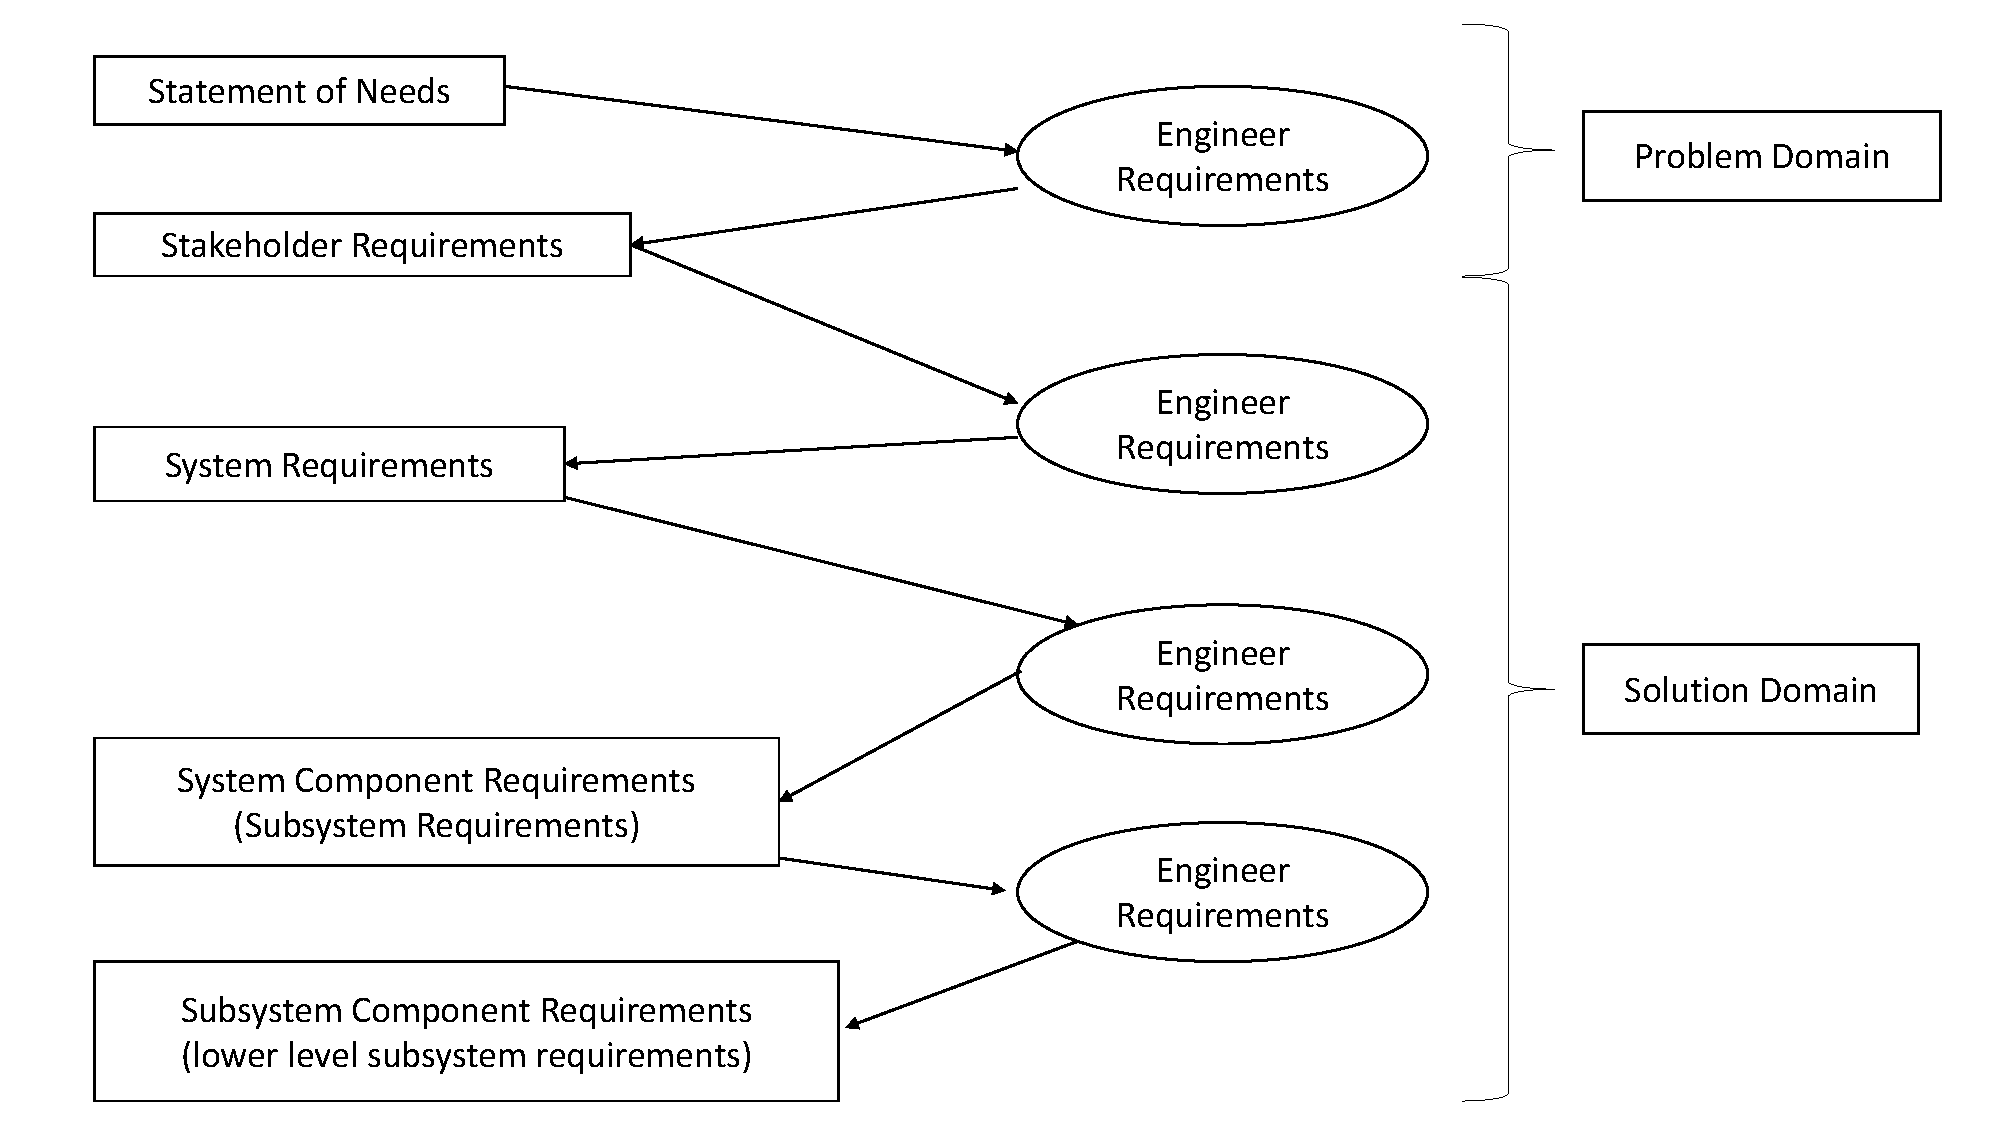
\includegraphics[scale=0.38]{img/levels-of-requirements-engineering.pdf}
	\caption{Entwicklungsprozess der Anforderungen}
	{\footnotesize \cite[Quelle: in Anlehnung an ][S.\,28]{hull_requirements_2011}}
	\label{abb:entwAnforderung}
	%		{\scriptsize \textit{Alle Rechte, einschließlich der Vervielfältigung, Veröffentlichung, Bearbeitung und Übersetzung bleiben der SV Informatik GmbH vorbehalten.}}
\end{figure}

Das \enquote{statement of needs} ist der Startpunkt für die Entwicklung einer Anforderung, die am Ende des Prozesses, der in Abbildung \vref{abb:entwAnforderung} dargestellt ist, präzise dokumentiert sein wird. Dieses ist am Anfang immer Ausdruck eines Anspruchs oder Wunsches an das zu entwerfende System; dabei bilden das \enquote{statement} und die \enquote{stakeholder requirements} die \enquote{problem domain}. Diese definiert die grundständige Methodik, wie auch eine nicht-technische Herangehensweise, die auf die Projektbeteiligten (\enquote{stakeholder}) angepasst sind. Nachfolgend werden die Projektbeteiligen als \enquote{stakeholder} bezeichnet. Die Rolle ist beschrieben als \enquote{(Stakeholder) sind Personen oder Organisationen, die ein potenzielles Interesse an einem zukünftigen System haben und somit in der Regel auch Anforderungen an das System stellen.}\autocite[][S.\,8]{partsch_requirements-engineering_2010} Später definiert die \enquote{problem domain} den Zweck des Systems: Dadurch ist bei der Ermittlung der Anforderungen die Frage \enquote{Was ist der Zweck des Systems?} anstelle \enquote{Was soll das System Ihrer Meinung nach tun?}. Dies soll die \enquote{stakeholder} extrinsisch motivieren, über den Zweck des zu entwerfenden Systems und nicht über einen möglichen Lösungsweg (das Wie) nachzudenken. Durch diesen Ansatz folgen Antworten nach dem Muster \enquote{Ich möchte etwas tun können ...}. Wissenschaftlich bzw. literarisch betrachtet sind diese Form der Anforderungen als \enquote{capability requirement(s)}\autocite[vgl.][S.\,94]{hull_requirements_2011} bekannt. Sie stellen die wichtigsten Erkenntnisse in der \enquote{problem domain} dar. Nun wird im weiteren Verlauf ein Modell konstruiert, das den Projektbeteiligten, den \enquote{stakeholder}, präsentiert wird. Dies unterliegt der Einschränkung, dass es jede/jedem Projektbeteiligte/-n versteht. Denn sie validieren das konstruierte Modell in jedem weiteren Schritt, der in Abbildung \vref{abb:entwAnforderung} ersichtlich ist. Die Anforderungen an das Modell sind quantitativ gering: Es muss nicht-technisch sein und es muss geeignet sein, die Anforderungen an das System abzubilden. Eine solche Darstellung ist dann geeignet, wenn sie den gewünschten Zweck an das System abbildet, das heißt, dass sie keine technischen Details zeigt, sondern einen Überblick bietet. Ein \enquote{use scenario}\autocite[vgl.][S.\,94]{hull_requirements_2011} wird meist verwendet, da es sich eignet, menschliche Aktionen bzw. Ziele darzustellen. Abschließend müssen die \enquote{stakeholder}-Anforderungen folgende Kriterien erfüllen: 

\begin{itemize}
	\item Kurz und prägnant formulierte Beschreibung, jedoch einfach zu verstehen und
	\item gleichzeitig sollten sie nicht-technisch, aber realistisch formuliert sein.
\end{itemize}
 
 Die \enquote{solutions domain}, die auf Abbildung \vref{abb:entwAnforderung} zu sehen ist, ist die Nachfolgerin der \enquote{problem domain}. Der Hauptunterschied zwischen den beiden Bereichen ist, dass die \enquote{solution domain} idealtypisch qualitativ hochwertig beschriebene Anforderungen als \enquote{Input} bekommt. Dazu konträr erhält die \enquote{problem domain} eine vage formulierte Wunschliste oder ein nicht klar definiertes Ziel als initialen \enquote{Input}. Ausgehend von der Aussage von E. Hull, \enquote{in an ideal world, all the requirements would be clearly articulated, individual testable requirements}\autocite[][S.\,115]{hull_requirements_2011}, ist zu deduzieren, dass es viele Ebenen zu erforschen gibt, um dieser Aufforderung zu entsprechen. So muss iterativ in jeder Ebene eine neue Analyse des \enquote{Inputs} erfolgen, um einen Ausgangspunkt für das weitere Vorgehen zu initialisieren. Die Komplexität dieser Ebenen ist abhängig von dem Grad der Innovation sowie vom Kontext des zu entwickelnden Systems. Jede Entscheidung während des Prozesses kann mögliche Entscheidungspfade in einer anderen Ebene verhindern. Ziel des Prozesses ist es, ein Anforderungsdokument bzw. -katalog zu entwerfen, das laut der gesichteten Literatur in verschiedenen Repräsentationen vorliegen kann. Dennoch sollten primäre Bestandteile, wie die Rahmenbedingungen, die Projektbeteiligten, die Projektaspekte und die funktionalen und nicht-funktionalen Anforderungen enthalten sein. Ein Beispiel dieses Katalogs ist im Anhang \vref{appendixAnforderung} zur Ansicht enthalten. Außerdem gibt es im Bereich der \enquote{Cloud} besondere architektonische Anforderungen. Diese sind im Anhang als Abbildung \vref{abb:cloudreq} einzusehen.
 
\subsection{\enquote{\ac{Cloud-C}}}
\ac{Cloud-C}, definiert als: \enquote{Paradigma, einen netzwerkbasierten Zugang auf ein skalierbares und  elastisches Reservoir gemeinsam nutzbarer physikalischer oder virtueller Ressourcen nach dem Selbstbedienungsprinzip und bedarfsgerechter Administration zu ermöglichen}\autocite[][S.\,7]{dindeutsches_institut_fur_normung_informationstechnik_2020-2}, ist ein neuartiger und disruptiver Ansatz in der Informationstechnologie, der seit mehreren Jahren Führungskräfte und IT-Abteilungen beschäftigt. Dieser Ansatz verspricht die Lösung für sämtliche Herausforderungen der Kapazitäts- und Leistungsengpässe moderner IT-Infrastruktur zu sein.\autocite[vgl.][S.\,4]{reinheimer_cloud_2018} Auch diskutiert die Bevölkerung stark und meist auch sehr kontrovers über dieses Thema. Themen wie Datenschutz,  Privatsphäre und das Risiko eines Datendiebstahls sind auch nach 20 Jahren Diskussion immer noch allgegenwärtig. Ein Grund dafür ist die hohe Dynamik dieser Technologie, sowie die ständige Weiterentwicklung, die von großen Unternehmen wie \textsc{Microsoft}, \textsc{Google}, \textsc{Amazon} und \textsc{IBM} vorangetrieben werden. Momentan haben \textsc{Microsoft} und \textsc{Amazon} die meisten Marktanteile am Umsatz im Bereich des \ac{Cloud-C}.\footnote{siehe dazu Abbildung \vref{abb:marktanteileCC19}} Des Weiteren prognostiziert \cite{gartner_cloud_2019} einen exponentiell wachsenden weltweiten Umsatz bis 2022 auf ungefähr 354,6 Milliarden US-Dollar. Damit würde dieser in den nächsten zwei Jahren um circa 100 Milliarden US-Dollar steigen. Für eine ausführliche Umsatzprognose ist auf die Abbildung \vref{abb:umsatzprognoseCC} zu verweisen. Diese verdeutlicht auch, dass in den folgenden Jahren nach 2022 weiterhin mit einer exponentiellen Umsatzsteigerung zu rechnen ist, wenn das mathematische Modell der exponentiellen Regression weiterhin Bestand hat. 
\par
Historisch betrachtet leitet sich \ac{Cloud-C} von verschiedenen Konzepten anderer \enquote{Comput-ing}-Bereiche und Architekturmuster ab: So spielte zur Entwicklung des heutigen Verständnis \enquote{Utility Computing}, \enquote{Service Orientation} und \enquote{Grid Computing} eine große Rolle.\autocite[vgl.][S.\,3-5]{hill_guide_2013} John McCarthy hat in den 1960er-Jahren das erste Konzept im Bereich des \enquote{Utility Computing} entwickelt.\autocite[vgl.][]{mccarthy_reminiscences_1983} Später wurde es durch Douglas Parkhill verfeinert und durch die folgenden Schlüsselkomponenten beschrieben: \enquote{Parkhill examined the nature of utilities such as water, natural gas and electricity in the way they are provided to create an understanding of the characteristics that computing would require if it was truly a utility. When we consider electricity supply, for example, in the developed world, we tend to take it for granted that the actual electrical power will be available in our dwellings. To access it, we plug our devices into wall sockets and draw the power we need. Every so often we are billed by the electricity supply company, and we pay for what we have used}.\autocite[vgl.][]{parkhill_challenge_1966} Dieses Konzept leitete er auch auf eine technologische Ressource im Bereich des Computers ab.\autocite[vgl.][S.\,4]{hill_guide_2013} Der Gedanke der Serviceorientierung beschreibt eine klare Begrenzung einer Funktion, die zur Erfüllung eines bestimmten Ziels verwendet wird. Services werden meist durch die Konzepte der Objektorientierung und der Abstraktion in einer Organisation definiert. Aus dem Grundgedanken und den genannten Konzepten entwickelt sich die \ac{SOA}, die diese Prinzipien in ein technologiebasiertes Modell abbildet. Die Leitgedanken der \ac{SOA} spielen auch im \ac{Cloud-C} eine wichtige Rolle, denn, wie später noch näher definiert wird, ist der Servicegedanke ein elementarer Bestandteil der \enquote{Cloud}, der deutlich das Geschäftsmodell prägt. \enquote{Grid Computing} ist ein Konzept aus den 1990er-Jahren und fand seine Anwendung im Bereich der elektrischen Netze.\autocite[vgl.][]{weinhardt_cloud_2009} Ziel dieses Konzeptes war es, die Einfachheit und Zuverlässigkeit der Stromnetze zu gewährleisten, über einen standardisierten Adapter Zugriff auf dieses zu erhalten, ohne sich um die technische Realisierung kümmern zu müssen. Dabei stellten die Pioniere dieses Konzeptes folgende Eigenschaften\autocite[vgl.][]{foster_grid_1999} an das System:

\begin{itemize}
	\item Dezentrale Ressourcenkontrolle, d.\,h., ein Grid besteht aus geografisch verteilten Ressourcen, die administrativ unabhängig von Organisationen betreut werden.	
	\item Standardisierte, offene Protokolle und Schnittstellen, d.\,h.; die Grid-Middleware
	ist nicht anwendungsspezifisch und kann zu verschiedenen Zwecken eingesetzt
	werden.
	\item Nichttriviale Eigenschaften des Dienstes, z. B. in Bezug auf Antwortzeitverhalten, Verfügbarkeit oder Durchsatz.
\end{itemize}
Diese Prinzipien haben eine Ähnlichkeit zu denen des \ac{Cloud-C}, jedoch sind die wirtschaftlichen Aspekte durch die Gedanken des \enquote{Grid Computing} beschrieben. Des Weiteren werden die Aspekte des \enquote{Grid Computings} im Bereich des dezentralen Managements und der verteilten Ressourcen beim \ac{Cloud-C} nicht weiterverfolgt. Vielmehr bietet die Zentralisierung die ökonomischen Vorteile, die eine zentrale Rolle des Geschäftsmodells darstellen. \par
Da es mehrere Definitionen von \ac{Cloud-C} gibt, beschränkt sich diese Arbeit auf folgende: \enquote{Cloud computing is a model for enabling ubiquitous, convenient, on-demand network access to a shared pool of configurable computing resources (e.g., networks, servers, storage, applications, and services) that can be rapidly provisioned and released with minimal management effort or service provider interaction. This cloud model is composed of five essential characteristics, three service models, and four deployment models.}\autocite[][S.\,2]{mell_nist_2011} Das \ac{NIST} beschreibt in der Publikation \cite{mell_nist_2011} folgende essenzielle Charakteristika\footnote{Jedoch werden diese Charakteristika in anderen wissenschaftlichen Ausarbeitungen um \enquote{multitenancy}, \enquote{service oriented} und \enquote{utility-based pricing} ergänzt.\autocite[vgl.][S.\,1]{institute_of_electrical_and_electronics_engineers_cloud_2011}}: 

\begin{itemize}
	\item on-demand self-service
	\item broad network access
	\item resource pooling
	\item rapid elasticity
	\item measured service
\end{itemize}
Des Weiteren beschreibt die \ac{NIST} drei Servicemodelle, wie sich Unternehmen die \enquote{Cloud} zunutze machen können: \ac{SaaS}, \ac{PaaS} und \ac{IaaS}. Dabei wird \ac{SaaS} definiert als: \enquote{The capability  provided to the consumer is to use the provider’s applications running on a cloud infrastructure. [...] The consumer does not manage or control the underlying cloud infrastructure including network, servers, operating systems, storage, or even individual application capabilities, with the possible exception of limited user-specific application configuration settings.}\autocite[][S.\,2]{mell_nist_2011} \enquote{Cloud}-Infrastruktur ist eine Sammlung von Hard- und Software des \enquote{Cloud}-Anbieters, die die fünf essenziellen Charakteristika des \ac{Cloud-C} unterstützt bzw. erfüllt. Beispiele hierfür sind \textsc{Google Docs} und \textsc{Office 365}. \ac{PaaS} wird beschrieben durch: \enquote{The capability provided to the consumer is to deploy onto the cloud infrastructure consumer-created or acquired applications created using programming languages, libraries, services, and tools supported by the provider. The consumer does
not manage or control the underlying cloud infrastructure including network, servers, operating systems, or storage, but has control over the deployed applications and possibly configuration settings for the application-hosting environment.}\autocite[][S.\,2]{mell_nist_2011} Bei der später in der Konzeptionierung verwendeten Software, \textsc{OpenShift}, handelt es sich um eine \ac{PaaS}-Lösung. Weitere Beispiele sind 
\textsc{Google App Engine}, \textsc{Windows Azure} und \textsc{Heroku}.\autocite[vgl.][S.\,8]{kumar_reliability_2018} \ac{IaaS} wird durch folgende Definition abgebildet: \enquote{The capability provided to the consumer is to provision processing, storage, networks, and other fundamental computing resources where the consumer is able to deploy and run arbitrary software, which can include operating systems and applications. The consumer does not manage or control the underlying cloud infrastructure but has control over operating systems, storage, and deployed applications; and possibly limited control of select networking components (e.g. host firewalls).}\autocite[][S.\,3]{mell_nist_2011} Hierzu zählen die Produkte \textsc{Amazon EC2}, \textsc{OpenStack} und \textsc{VMware}. Nun sind die Bereitstellungsmodelle der \enquote{Cloud} noch von Bedeutung: Die \ac{NIST} sowie weitere, schon für diesen Abschnitt verwendete, Literatur definieren vier Modelle: \enquote{private, community, public and hybrid cloud}. Die \enquote{private cloud} ist in exklusiver Nutzung eines Unternehmens, das mehrere interne Konsumenten bedient. Es kann entscheiden, ob alle Management- und Betriebsoperationen intern oder extern von einem Anbieter durchgeführt werden. Die \enquote{Cloud} kann intern oder extern gehostet sein. Die \enquote{community cloud} ist eine \enquote{private cloud}, jedoch unterscheiden sich die beiden durch die Benutzergruppen. Bei der \enquote{community}-Variante ist es nicht auf die Organisation, sondern auf Gruppen mit gleichen Angelegenheiten beschränkt. Die \enquote{public cloud} ist offen für die Öffentlichkeit --  natürlich beschränkt durch die Regeln des \enquote{Cloud}-Anbieters. Die hybride Variante wird folgendermaßen beschrieben: \enquote{The cloud infrastructure is a composition of two or more distinct cloud infrastructures (private, community, or public) that remain unique entities, but are bound together by standardized or proprietary technology that enables data and application portability (e.g., cloud bursting for load balancing between clouds).}\autocite[][S.\,3]{mell_nist_2011}


\subsection{Container, Containerisierung und Orchestrierung}\label{kap:container}
\enquote{Historically, virtualization technologies have developed out of the need for scheduling processes as manageable container units. The processes and resources in question are the file system, memory, network, and system information.}\autocite[][S.\,25]{pahl_containerization_2015} Aus dieser Notwendigkeit heraus entstanden verschiedene Lösungsansätze: die Virtualisierung in einer virtuellen Maschine (\ac{VM}) und etwas später die Container-Lösungen. Virtuelle Maschinen konnten einige Herausforderungen, wie \enquote{scheduling, packaging and resource access}, durch ihre technologischen Ansätze lösen. Dabei wurde der architektonische Ansatz des sogenannten \enquote{Gast Systems} entwickelt, d.\,h., die virtuelle Maschine ist ein vollwertiges \ac{OS} mit komplettem Dateisystem und eigenem Prozess auf dem \enquote{Host System}\footnote{Bietet Services für die Gastsysteme an.}. Im Vergleich dazu können Container die gleichen Anforderungen abbilden, jedoch unterscheidet sich deren Architektur (vgl. Abbildung \vref{abb:virutalizationArch}). Ein Container enthält alle notwendigen, für die App relevanten, Bibliotheken beziehungsweise Abhängigkeiten und kann so, ohne ein komplettes \ac{OS}, lauffähige Applikationen beinhalten. Diese Abstraktion ist im \enquote{Cloud}-Umfeld (bspw. in einer \ac{PaaS}-Ausprägung) nützlich, da die Container leichtgewichtiger sind und dadurch weniger Speicherauslastung (persistenter Speicher) benötigen. Auch später für die Orchestrierung der Container in einem Cluster-Umfeld ist dies von Nutzen. 

\begin{figure}[h!]
	\centering
	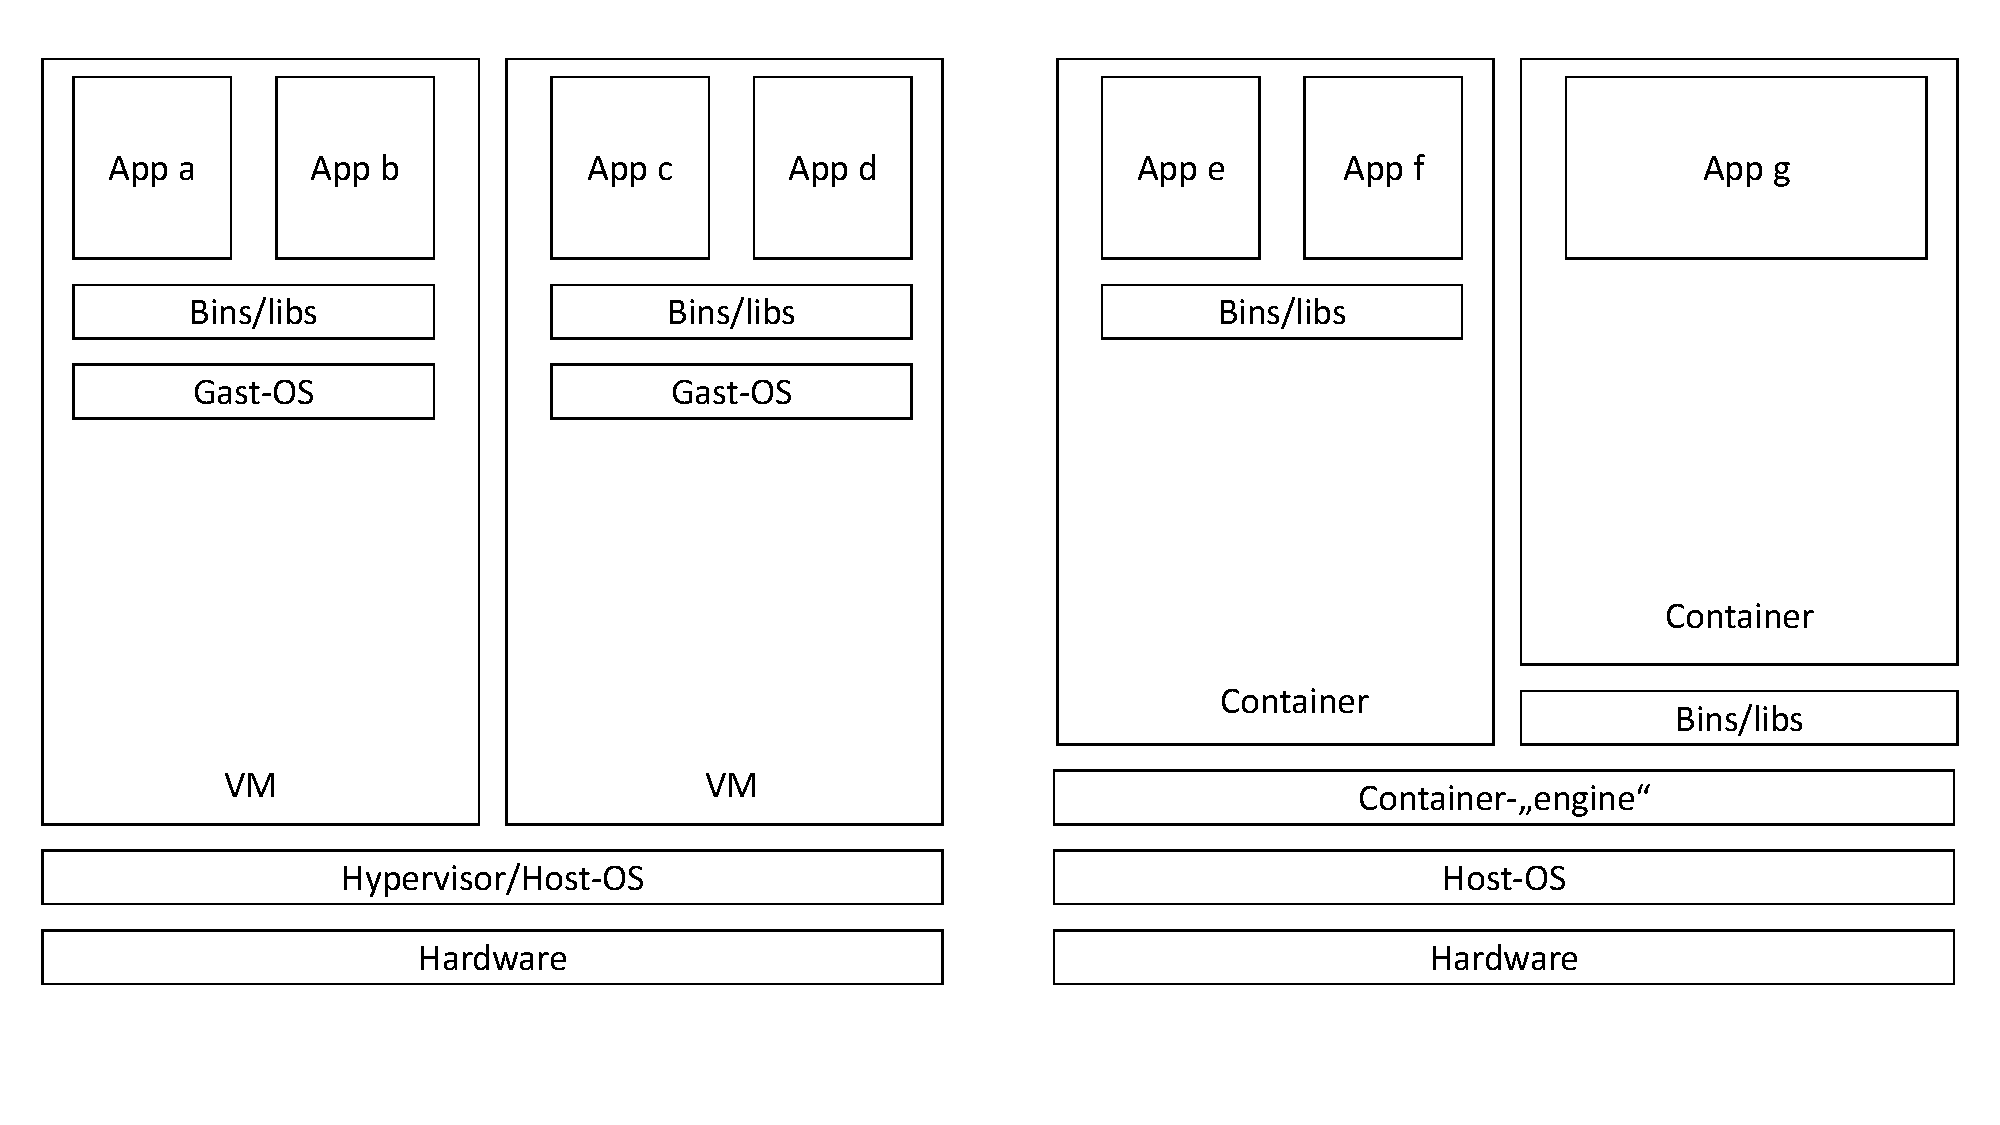
\includegraphics[scale=0.44]{img/virtualization architecture.pdf}
	\caption{Architektur der Virtualisierungsmodelle: VM vs. Container}
	{\footnotesize Quelle: in Anlehnung an \cite{pahl_containerization_2015}}
	\label{abb:virutalizationArch}
	%		{\scriptsize \textit{Alle Rechte, einschließlich der Vervielfältigung, Veröffentlichung, Bearbeitung und Übersetzung bleiben der SV Informatik GmbH vorbehalten.}}
\end{figure}

Die gesichtete Literatur (\cite{pahl_containerization_2015}, \cite{bernstein_containers_2014}, \cite{kharb_automated_2016}; \cite{combe_docker_2016} und weitere, siehe Literaturverzeichnis) definieren Container immer anhand ihrer charakteristischen Merkmale und im Vergleich zur \ac{VM}. \cite{google_ireland_limited_container_2020} folgt auch diesem Muster, allerdings eher auf Makroebene: \enquote{Container bieten einen logischen Mechanismus der Paketerstellung, der darauf beruht, dass Anwendungen von ihrer Ausführungsumgebung abstrahiert werden. Mit dieser Entkopplung können containerbasierte Anwendungen einfach und konsistent bereitgestellt werden, unabhängig davon, ob es sich bei der Zielumgebung um ein privates Rechenzentrum, die öffentliche \enquote{Cloud} oder auch um den persönlichen Laptop eines Entwicklers handelt.}\autocite[][]{google_ireland_limited_container_2020} Ziel der Containerisierung ist es, Entwicklerinnen die Möglichkeit zu bieten, sich nur auf die Anwendungslogik und -abhängigkeiten zu konzentrieren. Gleichzeitig können andere IT-Teams, wie \ac{IE2}, sich um die Bereitstellung und Verwaltung dieser Container kümmern. Diese Teams können den Container als geschlossene Verpackung sehen, bei der sie keine Kenntnis über das Innenleben (die Anwendungsdetails) für ihre Arbeit benötigen.\autocite[vgl.][]{google_ireland_limited_container_2020} Dies ist ein Bestandteil der Grundlagen für schnellere und qualitativ hochwertigere Deployments.\autocite[vgl.][S.\,1]{kharb_automated_2016} \par
Initial entwickelte \cite{canonical_ltd_linux_2020} die \ac{LXC}; \textsc{Docker Inc.} ist ein \enquote{Open source}-Projekt, das sich die \ac{LXC}-Technologie zunutze macht und eine Container-\enquote{Engine} gebaut hat, um diese Technologie benutzerfreundlicher zu gestalten: \enquote{Basically, \textsc{Docker} extends LXC with a kernel- and application-level API that together run processes in isolation: CPU, memory, I/O, network, and so on. \textsc{Docker} also uses namespaces to completely isolate an application’s view of the underlying operating environment, including process trees, network, user IDs, and file systems.}\autocite[][S.\,82]{bernstein_containers_2014} \textsc{Docker}-Container nutzen eine \enquote{Image}-Struktur. So lassen sich durch Kombination verschiedener \enquote{Images} Applikationen abbilden, die durch Programmierlogik ergänzt werden (vgl. Abbildung \vref{abb:containerArch}). In der Industrie ist \textsc{Docker} als De-facto-Standard\autocite[vgl.][S.\,30]{pahl_containerization_2015} angesehen\autocite[vgl.][S.\,1]{kharb_automated_2016}. Außerdem bietet \textsc{Docker} viele Vorteile, wie die Leichtgewichtigkeit, \enquote{Open source} und Sicherheit. Des Weiteren bietet \textsc{Docker} die Möglichkeit der Kollaboration zwischen verschiedenen IT-Teams. Weitere Vorteile sind, dass die Applikation überall (wo \textsc{Docker} installiert ist) ausgeführt werden kann und, dass \textsc{Docker} sich an die Unternehmensanforderungen ständig neu anpasst.\autocite[vgl.][S.\,1]{kharb_automated_2016} Durch diese Vorteile entstehen unmittelbare Konsequenzen, die Auswirkungen auf das Arbeiten haben: So werden das Einarbeiten eines neuen Mitarbeitenden beschleunigt, die Kreativität der Entwicklerinnen verstärkt, die Entwicklungsumgebung vereinheitlicht\footnote{Dies wirkt sich direkt auf die Code-/Produktqualität aus}, die Zusammenarbeit zwischen verschiedenen Teams vereinfacht und eine schnelle \enquote{\ac{TTM}}\footnote{\enquote{TTM is the strategy of focusing on reducing the time to introduce new products to market.} (\cite[][S.\,14]{pawar_time_1994})} erreicht.\autocite[vgl.][S.\,2]{kharb_automated_2016} 
\par 
Um die Stärken und Vorteile der \textsc{Docker}-Container zu nutzen, brauchen diese eine Netzwerkanbindung. Nur mit dieser können Container in der Produktion eingesetzt und eine Orchestrierung möglich gemacht werden. Dieser Begriff ist aus der Musik abgeleitet: Flexibles Kombinieren mehrerer Services oder Dienste zu einer sinnvollen Konzeption (Komposition), die einen Geschäftsprozess beschreibt. Für die Orchestrierung von Container-Anwendungen wird eine weitere Technologie benötigt, die von \cite{google_llc_production-grade_2020} entwickelt und als \enquote{Open source} veröffentlicht wurde: \ac{K8s}\footnote{\enquote{Is an open-source system for automating deployment, scaling, and management of containerized applications.} (\cite{google_llc_production-grade_2020})}. Die Semantik des Wortes \textsc{Kubernetes} bedeutet auf Griechisch \enquote{Lotse, Steuermann}. Diese Metapher beschreibt die Hauptaufgaben von \ac{K8s} zu treffend; es \enquote{verdeckt die Hardwareinfrastruktur und stellt ihr gesamtes Rechenzentrum als eine einzige, enorme Rechenressource dar. Dadurch können sie ihre Softwarekomponenten	bereitstellen und ausführen, ohne sich darum zu kümmern, welche Server konkret unterhalb dieser Schicht laufen. Bei der Bereitstellung von Anwendungen mit mehreren Komponenten wählt \textsc{Kubernetes} für jede dieser Komponenten einen Server aus, stellt sie bereit und ermöglicht es ihr, die anderen Komponenten zu finden und mit ihnen zu kommunizieren.}\autocite[][S.\,4]{luksa_kubernetes_2018} Der Nutzen von \ac{K8s} wird bei einer großen \enquote{Cloud}-Anbieterin, wie \ac{AWS} u. a., maximiert, da es den Entwicklerinnen ermöglicht, die Ausführung und Bereitstellung von Anwendungen entkoppelt von den Systemadministratorinnen zu betreiben.\autocite[vgl.][S.\,4]{luksa_kubernetes_2018} Eine grundlegende Übersicht einer \textsc{Kubernetes}-Architektur ist im Anhang \vref{abb:k8sArch} zu finden.
\par
\ac{K8s} führt einige Begrifflichkeiten ein, die nachfolgend einer Definition\autocite[][S.\,10-14]{caban_architecting_2019} (siehe Tabelle \ref{tab:definitionenK8s}) bedürfen. Diese werden im weiteren Verlauf dieser Arbeit benötigt, jedoch konzentriert auf die Forschungsfrage eins. Eine detailreiche Übersicht der Architektur der oben beschrieben Konzepte ist im Anhang \vref{abb:k8sArchInteraktion} zu sehen. Diese beschreibt das Zusammenwirkung der einzelnen Komponenten.
\par

\begin{longtable}[c]{@{}lp{12.0cm}@{}}
	\toprule[1.5pt]
	\textbf{Begriff} & \textbf{Definition} \\* \midrule
	\endfirsthead
	%
	\multicolumn{2}{c}%
	{{\bfseries Tabelle \thetable\ der vorherigen Seite fortgeführt.}} \\
	\toprule
	\textbf{Begriff} & \textbf{Definition} \\* \midrule
	\endhead
	%
	\bottomrule
	\endfoot
	%
	\endlastfoot
	%
	\enquote{Pod}              & \enquote{A Pod is a group of one or more tightly coupled Containers sharing a set of Linux namespaces and cgroups.} Innerhalb des \enquote{Pod} wird der Netzwerk-/\enquote{Mount}-Namensraum geteilt, dies ermöglicht die Kommunikationen innerhalb eines \enquote{Pod}. Mehrere dieser kommunizieren über \textit{localhost}. \\
	\enquote{Services}         & \enquote{A Service is a Kubernetes object that maps one or more incoming ports to targetPorts at a selected set of target of Pods. These represent a microservice or an application running on the cluster.} \\
	\enquote{Worker nodes}     & \enquote{The worker nodes (formerly known as minions) host elements like the kubelet, kube-proxy, and the container runtime.} Darin sind die \enquote{Pods} enthalten, welche die Container-Anwendungen beinhalten. \\
	\enquote{Master nodes}     & \enquote{The master nodes are the nodes hosting core elements of the control plane like (not an exhaustive list) the kubeapi-server, kube-scheduler, kube-controller-manager, and in many	instances the etcd database.} Diese übernimmt die Management-Aufgaben im Cluster. \\* \bottomrule
	
		
	\caption{Definition der \enquote{\ac{K8s}}-Begrifflichkeiten}\label{tab:definitionenK8s}\\
\end{longtable}


\section{Anforderungsanalyse des zu implementierenden Prozesses}
% Anforderungskatalog \vref{tab:anforderungslisteFF1}
% Formulierungshilfen für Anforderungen \autocite[][]{rupp_formulierungsregel_2020}
Das \enquote{statement of needs} ist, wie in Kapitel \vref{kap:methodikAnfAnalyse} beschrieben, ein Wunsch beziehungsweise Anspruch an das zu entwickelnde System (hier: ein Prozess): Es sollen Container-Anwendungen automatisiert auf die \textsc{OpenShift}-Umgebung verteilt werden. Dies soll von der dafür zuständigen Abteilung im Unternehmen übernommen werden, d.\,h. die Verantwortung dieses Prozesses wird übergeben. Ziel ist es, Aufgaben und Verantwortlichkeiten so zu verteilen, dass sie dem Aufbau- sowie Ablauforganisation entsprechen. Die Entwicklungsabteilungen/-teams möchten weiterhin nicht mehr für die Verteilung der Container-Anwendungen verantwortlich sein. Des Weiteren sprechen rechtliche Aspekte gegen dies, dass die Entwicklung auf Dauer Anwendungen in die \ac{PROD} verteilt. Bei näherer Betrachtung der oben genannten Gründe ist folgendes festzustellen: es sprechen rechtliche Voraussetzung und unternehmens-organisatorische Aspekte dafür, hier ein weiteres Vorgehen anzustreben. Alleinig durch die rechtlichen Aspekte muss eine Veränderung des IST-Zustands angestrengt werden, damit ist das Vorgehen begründet und die Ermittlung der Projektbeteiligten (\enquote{stakeholder}) kann durchgeführt werden.
\par
Die Projektbeteiligten sind im engeren Sinn die Fachbereiche (also Kunden der Anwendung), die Entwicklungsteams und die \enquote{Deployment}-Abteilung. So hat der Fachbereich Interesse an einem funktionsfähigen System, die Entwicklungsteams an einem häufigen (annäherungsweise kontinuierlichem) \enquote{Deployment} und die \enquote{Deployment}-Abteilung an einem hoch automatisiertem und revisionskonformen Prozess. Dies sind nur einige Aspekte, die bei weitem nicht alle Gründe des Interesses abdecken. Es werden hier nur die \enquote{stakeholder} im engeren Sinn weiter betrachtet, da diese Arbeit sich mit der Modellierung eines automatisierten Prozesses im Bereich der Entwicklung, der wirtschaftlichen Betrachtung und der rechtlichen Sicherung dieses beschäftigt. Der Fokus liegt auf der Modellierung des Prozesses und mit diesem deckt es die engeren Projektbeteiligten ab. 
\par
Nachfolgend wird der automatisierte \enquote{Deployment}-Prozess zur Verteilung von Containern als \textit{System} bezeichnet. Dies erfolgt auf der Grundlage der Formulierungshilfe für Anforderungen nach \cite{rupp_formulierungsregel_2020}. Es werden ausschließlich die funktionalen Anforderungen \autocite[vgl.][]{international_organization_for_standardization_isoiec_2011,} betrachtet, da die erfassten alle produkt-spezifisch sind -- nicht-funktionale Anforderung sind im Gegensatz dazu produkt-unspezifisch. Zur besseren Übersichtlichkeit sind die Anforderungen mit $A_{1}, A_{2}, ..., A_{n}, n \in \mathbb{N}$ nummeriert und ein Anforderungskatalog ist im Anhang \vref{tab:anforderungslisteFF1} zu finden. Die folgenden Anforderungen $A_{1}, A_{2}, ..., A_{8}$ stammen von dem Projektbeteiligten (\enquote{stakeholder}) \enquote{Entwicklungsteam/-abteilung}. Diese wurden während einer Befragung dieses Teams am 11.März 2020 im Rahmen einer Arbeitstagung \enquote{Container-Verteilung} erhoben. Die Anforderungen $A_{9}$ und $A_{10}$ beschreiben wichtige Bedingungen der Abteilung \ac{IE2}. 
\par 
$\mathbf{A_{1}}$\textbf{: Das System muss die Möglichkeit bieten, über eine korrekte Konfigurationsdatei, alle Komponenten der Anwendung zu verteilen.}
\par
Damit gewährleistet das System beziehungsweise der Prozess die Verteilung aller Komponenten ins \textsc{OpenShift}-Cluster. Dieses benötigt die Konfigurationsdatei, um die Anwendung zu betreiben. Die Verteilung in \textsc{OpenShift} funktioniert über diese Datei, damit werden nicht die fertigen Container direkt verteilt sondern es wird nur beschrieben welche Container wohin müssen. Danach übernimmt \textsc{OpenShift} die Beschaffung der Container.
\par
$\mathbf{A_{2}}$\textbf{: Das System soll die Möglichkeit bieten über eine standardisierte Übergabedatei alle Umgebungsvariablen des Containers zu definieren.}
\par
Diese Anforderung soll die Fehler in der Konfigurationsdatei minimieren, denn diese muss korrekt formatiert sein, sonst kann sie nicht richtig verarbeitet werden. Dabei spielen Einrückungen und Leerzeichen bei der Formatierung eine wichtige Rolle. Gleichzeitig birgt dieser Umstand großes Fehlerpotential. Mit der standardisierten Übergabedatei werden die Fehler mittels automatischem Einlesen und Generierung der Konfigurationsdatei -- zumindest die Formatierungsfehler -- verhindert. Dies hat keinen Einfluss auf fachliche Fehler, z.\,B. die Angabe einer falschen Umgebungsvariablen oder eine falsche Serveradresse der Versionskontrolle.
\par
$\mathbf{A_{3}}$\textbf{: Das System muss die Möglichkeit bieten, über eine Validierung, konsistente Komponenten zu verteilen.}
\par
Dies beschreibt eine Kontrollinstanz, die Fehler erkennen soll und dann die Verteilung abbrechen oder eine Benutzeraktion fordern soll. Die Fehlerbearbeitung muss nicht komplett automatisiert sein, da sie meist Einzelfälle behandelt und diese nicht nach dem selben Muster zu lösen sind. Die Verteilung wird nach Behebung der/des Fehler(s) fortgesetzt.
\par
$\mathbf{A_{4}}$\textbf{: Das System muss die Möglichkeit bieten unabhängig von dem Inhalt des Containers diesen zu verteilen.}
\par
$A_{4}$ beschreibt die Anforderung den Vorteil von Container-Anwendungen auszunutzen: Dieser ist die Möglichkeit beim Verteilen des Container den Inhalt ignorieren zu können, da der Container eine Abstraktionsebene darstellt.\footnote{vgl. dazu Kapitel \vref{kap:container}, dass die Funktionsweise und Vorteile genauer erläutert.} Die Entwicklungsabteilung möchte diese Vorteile nutzen, \enquote{da sonst die Umstellung auf Container wenig Sinn ergeben würde}, so ihre Aussage. Dies ist keine wissenschaftlich begründete Aussage und ist deswegen als direktes Zitat markiert.
\par
$\mathbf{A_{5}}$\textbf{: Das System muss fähig sein mit \textsc{OpenShift} über das \ac{API} zu kommunizieren.}
\par
Diese Anforderung ist ein Funktionswunsch, der es ermöglicht, mittels \ac{CLI}-Kommandos mit der Anwendung \textsc{OpenShift} zu kommunizieren. Dies hat den Vorteil die internen Möglichkeiten von \textsc{OpenShift} vollständig ausnutzen zu können, z.\,B. die interne Validierung von Konfigurationsdateien.
\par
$\mathbf{A_{6}}$\textbf{: Das System soll fähig sein das \textsc{OpenShift}-Cluster zu jedem Zeitpunkt mit einem konsistenten Zustand zu verlassen.}
\par
Mit dieser Forderung soll gewährleistet werden, dass das System die \textsc{OpenShift}-Umgebung nicht unbrauchbar macht und es so zur Produktionsverhinderung kommt. Dass würde bedeuten die Kunden haben kein lauffähiges System mehr und es würde zu Umsatzausfällen, Vertrauensverlust bei den Versicherungsnehmern u.\,a. kommen. 
\par
$\mathbf{A_{7}}$\textbf{: Das System wird die Möglichkeit bieten die Verteilung von Komponenten zu unterbrechen.}
\par
$A_{7}$ beschreibt die Forderung nach einer Notfallunterbrechung, die jedoch dem System und der \textsc{OpenShift}-Umgebung keinen Schaden zufügt. Dies soll, wie $A_{6}$, ein konsistentes System hinterlassen. 
\par
$\mathbf{A_{8}}$\textbf{: Das System muss die Möglichkeit bieten, über die zentrale Verteilungssoftware \textsc{Ara}, die Verteilung der Komponenten durchzuführen.}
\par
Diese Forderung widerspricht dem Anspruch nach \cite{hull_requirements_2011}, Anforderungen ohne Bezug zu einer bestimmten Anwendung beziehungsweise einer Technologie zu formulieren. Jedoch ist es eine zwingende Forderung der Abteilung \ac{IE2} diese Technologie zu verwenden. Es sollen alle Systeme/Prozesse mit dieser umgesetzt werden.
\par
$\mathbf{A_{9}}$\textbf{: Das System muss die Möglichkeit bieten automatisiert alle notwendigen Komponenten über die Konfigurationsdatei zu erkennen und zu verteilen.}
\par
Dies ist eine Anforderung an die Vollständigkeit der Konfigurationsdatei, die die benötigten Komponenten beschreibt. Wichtig dabei ist es, dass die Konfigurationsdatei nicht nur vollständig ist, sondern auch semantisch korrekt ist. Ein zentrales Akzeptanzkriterium ist, dass das System automatisiert funktioniert und bei Normalbetrieb keine menschliche Aufsicht benötigt.
\par
$\mathbf{A_{10}}$\textbf{: Das System muss den gesetzlichen sowie sicherheitstechnischen Vorgaben entsprechen.}
\par
$A_{10}$ beschreibt eine nicht-funktionale Anforderungen, die zwingend erforderlich ist und deswegen an dieser Stelle erwähnt wird. Im Bereich der Finanzdienstleistungen, welche das Versicherungswesen inkludieren, sind strenge Sicherheitsvorschriften und gesetzliche Rahmenbedingung einzuhalten (vgl. dazu die Forschungsfrage drei im Kapitel \vref{ff3}). Diese nicht-funktionale Anforderung ist an alle Vorhaben/Projekte gerichtet und wird von dem Projektbeteiligten \enquote{Geschäftsführung} eingebracht. Diese Anforderung muss zwingend umgesetzt werden. 

\section{Konzeption eines Container-basierten, automatisierten \enquote{Deployments}}
Dieses Teilkapitel beschreibt den Aufbau einer \textsc{OpenShift}-Labor-Umgebung, um das Verhalten von \textsc{OpenShift} zu testen. Des Weiteren wird eine Prozessmodellierung des automatisierten \enquote{Deployments} anhand einer Beispielanwendung \textsc{Camunda} erläutert. Dies ist gleichzeitig die Testapplikation, die in der \ac{SVI} benutzt wird, um das automatisierte \enquote{Deployment} von Container-Anwendungen zu untersuchen. Abschließend wird eine generische Konfigurationsdatei entwickelt, um Applikationen ins \textsc{OpenShift}-Cluster zu verteilen.

\subsection{Aufbau und \enquote{Deployment} eines \textsc{OpenShift}-Labors}
Nachfolgend wird der Aufbau einer \textsc{OpenShift}-Labor-Umgebung mit \enquote{single node}-Architektur beschrieben, d.\,h., es ist nur eine \enquote{worker node} im \textsc{OpenShift}-Cluster vorhanden. Dieses wird auf einem \textsc{Ubuntu}-System in der Version 18.04 installiert. Der folgende Quelltext \vref{lst:openShift} beschreibt die Terminal-Eingaben:

\begin{lstlisting}[language=bash, caption={Installation des \textsc{OpenShift}-Clusters}, label=lst:openShift]
curl -fsSL https://download.docker.com/linux/ubuntu/gpg | sudo apt-key add -
sudo add-apt-repository "deb [arch=amd64] https://download.docker.com/linux/ubuntu $(lsb_release -cs) stable"
sudo apt update && sudo apt -y install docker-ce
docker version
sudo usermod -aG docker $USER
wget $LINK
tar xvf openshift-origin-client-tools*.tar.gz
cd openshift-origin-client*/
sudo mv  oc kubectl  /usr/local/bin/
oc version 
cat << EOF | sudo tee /etc/docker/daemon.json 
{
"insecure-registries" : [ "172.30.0.0/16" ]
}
EOF
sudo systemctl restart docker
oc cluster up
\end{lstlisting}

Das Konzept dieses \enquote{Shell}-Skripts \vref{lst:openShift} ist es, zuerst die notwendigen Abhängigkeiten und danach die \textsc{OpenShift}-Anwendungen zu installieren. So werden in den Zeilen eins bis drei die notwendigen Voraussetzungen geschaffen, um die \textsc{Docker}-Umgebung zu installieren. Zuerst wird der \textsc{GPG}\footnote{\enquote{GnuPG is a complete and free implementation of the OpenPGP standard as defined by RFC4880 (also known as PGP). GnuPG allows you to encrypt and sign your data and communications; it features a versatile key management system, along with access modules for all kinds of public key directories.} Quelle: \cite{the_people_of_the_gnupg_project_gnu_2020}}-Schlüssel zum lokalen Schlüsselbund hinzugefügt, danach kann die Anwendung \textsc{Docker} mit dem \ac{APT}-Programm heruntergeladen und installiert werden. Danach wird getestet, ob die Installation von \textsc{Docker} erfolgreich war, und der eigene Benutzer wird der Gruppe \enquote{docker} hinzugefügt. Dies wird benötigt, um dem eigenen Benutzer die Steuerung der Software \textsc{Docker} zu erlauben. Die Zeilen sechs bis neun installieren \textsc{Kubernetes} und \textsc{OpenShift} (in der \enquote{Community}-Variante). Sehr wichtig sind die Anpassungen, die in den Zeilen elf bis fünfzehn vorgenommen werden: Sie fügen einen Eintrag \lstinline[language=bash]|"insecure-registries" : [ "172.30.0.0/16" ]| in die Datei \lstinline[language=bash]|/etc/docker/daemon.json| ein. Dies erlaubt es \textsc{Docker}, auf unsichere Verzeichnisse zuzugreifen; dadurch kann \textsc{OpenShift} lokal Container-\enquote{Images} im Cache speichern, um diese schneller wiederzuverwenden. Schließlich wird ein Cluster in \enquote{default}-Konfiguration zur Kontrolle der Funktionsfähigkeit mit \lstinline[language=bash]|oc cluster up| erstellt. Dies ist unter \lstinline[language=HTML, breaklines=true]|http://127.0.0.1:8443/console| als Web-Konsole erreichbar.
\par
Um das Verhalten des \textsc{OpenShift}-Clusters während eines \enquote{Deployments} zu testen, wird ein Test-Projekt erstellt. Grundsätzlich sind die meisten Kommandos der \ac{CLI} nach dem Muster \lstinline[language=sh]|oc <action> <object type> <obj name or id>|\autocite[vgl.][]{red_hat_inc_cli_2020} aufgebaut. Ein Projekt ist in \textsc{OpenShift} ein privater Bereich, indem Applikationen laufen können und nur die Erstellerin administrativen Zugriff besitzt. Dieser kann nach außen veröffentlicht werden, wenn dies erforderlich ist. Nachdem das Projekt mit \lstinline[language=bash]|oc new-project <projectName> --display-name '<displayName>'|\footnote{\enquote{<Platzhalter>}, die mit Werten vor der Ausführung ersetzt werden müssen.} erstellt wurde, wird dies automatisch als \enquote{default}-Projekt ausgewählt, d.\,h., darin werden nun alle folgenden Schritte ausgeführt. Des Weiteren ist die Überlegung zu treffen, ob noch weitere Benutzer für das angelegte Projekt eine Berechtigung erhalten (\lstinline[language=bash]|oc adm policy add-role-to-user <admin/edit/view> <collabUser>|). 
\par
Als Test-Applikation soll eine Webseite auf Basis von \textsc{Django}\footnote{\enquote{Django is a high-level Python Web framework that encourages rapid development and clean, pragmatic design.} Quelle: \cite[][]{django_software_foundation_web_2020}} in Cluster verteilt werden. Es wird ein vorgefertigtes \enquote{Image} für diesen Test genutzt. Der Quellcode \vref{lst:openShiftDeployLab} zeigt die benötigten Kommandos, um eine neue Applikation zu erstellen. Des Weiteren illustriert dieser, wie die Anwendung nach außen freigegeben wird, d.\,h., sie ist außerhalb des Projektes erreichbar. Danach wird in Zeile \vref{lst:line:testConn} der Quellcode-Abbildung \vref{lst:openShiftDeployLab} die Verbindung zur Webseite mittels der Ermittlung des \textsc{HTTP}-Status-Codes überprüft\footnote{Der Quelltext dieser Funktion ist im Anhang \vref{lst:testConnection} einzusehen.}.

\begin{lstlisting}[language=bash, caption={Test-\enquote{Deployment} ins \textsc{OpenShift}-Cluster}, label={lst:openShiftDeployLab}]
oc new-app openshiftkatacoda/blog-django-py --name blog
oc describe svc/blog # print config 
oc expose svn/blog
oc status | grep 'to pod port' # see all exposed services on this project

# test_connection is listed at @\vref{lst:testConnection}@
test_connection blog-lab.127.0.0.1.nip.io @\label{lst:line:testConn}@
\end{lstlisting}

Nach Abschluss des Tests wird die Applikation mit \lstinline[language=bash]|oc delete all --selector app=blog| wieder gelöscht.

\subsection{Modellierung einer \enquote{Deployment}-Konfigurationsdatei}
Um eine Verteilung der Container-Anwendung auf dem \textsc{OpenShift}-Cluster durchzuführen, benötigt das System eine Konfigurationsdatei, die als \ac{API}-Objekt an \textsc{OpenShift} übergeben wird. Dabei definiert diese den gewünschten Zustand einer bestimmten Komponente der Anwendung als \enquote{pod}\footnote{siehe Tabelle \vref{tab:definitionenK8s}}-Vorlage.\autocite[vgl.][Application\,$\rightarrow$\,Deployments]{red_hat_inc_okd_2019} Diese Datei stellt, als alleinige Quelle (\ac{SPOT}), alle notwendigen Informationen bereit, die die Anwendungen \textsc{OpenShift} benötigt, um eine funktionsfähige Datei in dem ausgewählten Projekt des Clusters bereitzustellen. Dies ist der erste Unterschied zum klassischen \enquote{Deployment} bei dem alle Quelldateien verteilt werden müssen.\autocite[vgl.][]{dearle_software_2007} Dabei ist die Konfigurationsdatei deklarativ\footnote{Programmierparadigma: im Gegensatz dazu gibt es das imperative Vorgehen, dass das \textit{Was} in welcher Reihenfolge zu tun ist beschreibt.} beschreiben, d.\,h. sie beschreibt \textit{was} \textsc{OpenShift} mit der angegeben Komponente machen soll.

Es gibt zwei verschiedene Ausprägungen der Konfigurationsdatei: \enquote{DeploymentConfig} und \enquote{Deployment}. Nachfolgend werden die Ziele, der Nutzen und ein Beispiel der Ausprägung beschrieben. Die \enquote{DeploymentConfig}-Variante ist von \textsc{Red Hat} für \textsc{OpenShift} entwickelt worden, um eine erweiterte Unterstützung für die Softwareentwicklung und den Lebenszyklus des \enquote{Deployments} zu unterstützen. Damit hat \textsc{Red Hat} ein eigenes Konzept entwickelt, wie die Verteilung von Software aussehen kann. Dieses Konzept bietet folgende Eigenschaften, die verschiedene Nutzungsmöglichkeiten ermöglichen:\autocite[vgl.][Application\,$\rightarrow$\,Deployments]{red_hat_inc_okd_2019}
\begin{enumerate}
	\item \enquote{A DeploymentConfig, which is a template for running applications.}
	\item \enquote{Triggers that drive automated deployments in response to events.}
	\item \enquote{User-customizable deployment strategies to transition from the previous version to the new version. A strategy runs inside a Pod commonly referred as the deployment process.}
	\item \enquote{A set of hooks (lifecycle hooks) for executing custom behavior in different points during the lifecycle of a deployment.}
	\item \enquote{Versioning of your application in order to support rollbacks either manually or automatically in case of deployment failure.}
	\item \enquote{Manual replication scaling and autoscaling.} 
\end{enumerate}
Allgemein definiert das \enquote{DeploymentConfig}-Objekt die Anzahl der Replikationen, beschreibt die Auslöser (\enquote{trigger}) für die automatische Erstellung von neuen \enquote{Deployments}; die Strategie, mit der die Übergange zwischen verschiedenen Versionsständen verwaltet sind, und Lebenszyklus-\enquote{Hooks}\footnote{Funktionen, die beim Eintreten eines bestimmten Events automatisch ausgelöst werden}. Wenn eine neue Verteilung von Komponenten angestoßen wird, aktiviert sich ein spezieller \enquote{pod}, um die die Verteilung zu überwachen und zu betreuen. Dieser fährt die alten Replikationen herunter, aktiviert neue und startet die \enquote{hooks}. Wichtig ist, dass er die alten Replikationen behält, um ein schnelles \enquote{rollback}, also eine Wiederherstellung des Zustands vor der aktuellen Verteilung, zu ermöglichen. Der Verteilungs-\enquote{pod} bleibt für unbestimmte Zeit im Cluster, damit die Logdatei nicht gelöscht wird. 

\lstinputlisting[language=yaml, caption={Beispiel einer \enquote{DeploymentConfig}-Datei}, label=lst:demoDeploymentConfig]{resources/listings/deploymentConfigDemo.yaml}

Dieser Quellcode \vref{lst:demoDeploymentConfig}\autocite[vgl.][Application\,$\rightarrow$\,Deployments]{red_hat_inc_okd_2019} zeigt eine Ausprägung der \enquote{DeploymentConfig}. Die Zeilen 10\,ff. beschreibt typische \enquote{trigger}, die bei einem gewissen Ereignis ausgelöst werden. Die Bezeichner beschreiben die Funktionsweise ausreichend. Die Verteilungsstrategie wird durch die Zeilen 20\,f. eingestellt. Hier wird die Strategie \enquote{rolling} verwendet, d.\,.h die einzelnen \enquote{pods} einer/mehrerer \enquote{worker node(s)} werden während dem laufenden Betrieb unbemerkt gegen die neue Version getauscht -- die Endanwenderin bekommt davon nichts mit. Im Gegensatz zu der Variante \enquote{DeploymentConfig} gibt es die \acl{K8s}-Version \enquote{Deployment}, die kompatibel mit \textsc{OpenShift} ist. Sie werden als Nachkomme der \textsc{OpenShift}-Variante (\enquote{DeploymentConfig})\autocite[vgl.][Application\,$\rightarrow$\,Deployments]{red_hat_inc_okd_2019} bezeichnet. Die \enquote{Deployment}-Ausprägung beschreibt, wie die \enquote{DeploymentConfig}, den gewünschten Zustand einer Anwendungskomponente in Form einer \enquote{pod}-Vorlage. Der Quellcode \vref{lst:demoDeployment}\autocite[vgl.][Application\,$\rightarrow$\,Deployments]{red_hat_inc_okd_2019} erzeugt bei der Ausführung im \textsc{OpenShift}-Cluster eine Replikation des \enquote{hello-openshift}-\enquote{pod}.

\lstinputlisting[language=yaml, caption={Beispiel einer \enquote{Deployment}-Datei}, label=lst:demoDeployment]{resources/listings/deploymentDemo.yaml}

Dabei spezifizieren die Zeilen 16-17, welches \textsc{Docker}-Abbild als Container geladen wird. Die Zeile 19 gibt den Port 80 für die Kommunikation innerhalb des \enquote{pod} frei.
\par
Beide Konfigurationsdatei-Ausprägungen sind vollständig nutzbar in der Anwendungen \textsc{OpenShift}, um eine Verteilung von Komponenten zu beschreiben und auszuführen. \textsc{Red Hat} empfiehlt die Variante \enquote{Deployment} zu nutzen unter der Einschränkung, dass keine Funktionen beziehungsweise kein Verhalten benötigt wird, welches nur die \enquote{DeploymentConfig}-Variante bietet.\autocite[vgl.][Application\,$\rightarrow$\,Deployments]{red_hat_inc_okd_2019} Nachfolgend soll betrachtet werden, welche der möglichen Varianten für die \ac{SVI}, begründet durch die Anforderungen der \enquote{stakeholder}, sinnvoll erscheint. Zuvor werden die beiden Möglichkeiten verglichen und die Unterschiede hervorgehoben: Die Varianten unterschieden sich in einem Punkt sehr stark -- dem Design. Genauer formuliert unterscheiden sie sich in der Eigenschaftsauswahl des CAP-Theorem\footnote{\enquote{The CAP theorem states that any networked shared-data system can have at most two of three desirable properties: consistency (C) equivalent to having a single up-to-date copy of the data; high availability (A) of that data (for updates); and tolerance to network partitions (P).}\autocite[][S.\,1]{brewer_cap_2012} CA macht keinen Sinn, da nicht jeder Client dieselben Daten sehen kann und gleichzeitig immer erreichbar ist.}, so bevorzugt die \enquote{DeploymentConfig}- \enquote{consistency} während die \enquote{Deployment}-Variante \enquote{availability} bevorzugt. Übersetzt bedeutet das, wenn der Verteiler-\enquote{pod} während des \enquote{rollouts} der \enquote{DeploymentConfig} einen Fehler aufweist, wartet der komplette Prozess bis die \enquote{node} mit dem \enquote{pod} wieder aktiv wird oder manuell gelöscht wird. Während dieser Phase stockt der Prozess und es wird kein Fortschritt erreicht. Im Gegensatz dazu wird die Verteilung der \enquote{Deployment}-Variante über einen sogenannten \enquote{controller}-Manager durchgeführt, der als Hochverfügbarkeitslösung implementiert ist, d.\,h. die Verfügbarkeit (\enquote{availability}) steht an erster Stelle. Diese Überlegung muss im Rahmen der Prozessmodellierung als erstes in der \ac{SVI} vollzogen werden, um danach die spezifischen Funktionsunterschiede der beiden Konfigurationsdateien weiter zu beleuchten. 
\par
In einer Arbeitstagung zum \ac{PoC} des \textsc{OpenShift}-Systems haben die Entwicklerinnen einen ersten Entwurf für die Konfigurationsdatei vorgestellt. Hier wurde die Version \enquote{Deployment} verwendet -- begründet war dies durch das Argument, dass keine Funktionen der \enquote{DeploymentConfig}-Version benötigt wurden (Dies ist konform zur Aussage von \textsc{Red Hat}\autocite[vgl.][Application\,$\rightarrow$\,Deployments]{red_hat_inc_okd_2019}). Im Anhang \vref{lst:entwurfCamunda} ist die vollständige Version abgedruckt. Wichtig für den \enquote{stakeholder} Entwicklerin ist, die Beschreibung der Umgebungsvariablen, die die Anwendung braucht, um mit zusätzlichen Webservices zu kommunizieren. Der Quellcode \vref{lst:deploymentCamundaEnv} zeigt diese Stelle nochmals, die einer besonderen Analyse bedarf. Es soll ein Algorithmus zur Generierung der Konfigurationsdateien entwickelt werden. Ziel dieses ist es, mögliche Fehler bei der manuellen Erstellung der Datei zu verhindern und ein vollständig automatisierten Prozess zu entwickeln. Die Generierung mittels Programmlösung ist eine Bedingung der Abteilung \ac{IE2}, die die Verantwortung für die Verteilung der Anwendungen tragen.

\lstinputlisting[language=yaml, firstline=17, lastline=42, firstnumber=17, caption={Ausschnitt aus Quellcode \ref{lst:entwurfCamunda}: Deklaration der Umgebungsvaribalen}, label=lst:deploymentCamundaEnv]{resources/listings/camundaEnv.yaml} 

Die Zeichenketten mit dem Muster \enquote{\textit{\$Bezeichner\_}} stellen Platzhalter dar, die genutzt werden, um die eigentlichen Werte nicht in Klartext abzudrucken. Diese fallen unter das Betriebsgeheimnis. Platzhalter mit der gleichen Zeichenkette haben den identischen Inhalt. Es fällt auf, dass die \ac{URL} der Webservices immer mit dem gleichen Host beginnt und ein Teil des Pfades auch gleich ist. Es gibt zwei Möglichkeiten, wie der Algorithmus zur Generierung der Konfigurationsdateien aussehen könnte: Bei der \enquote{Deployment}-Variante müsste dieser die komplette Datei anhand definierter Regeln generieren. Die zweite Möglichkeit ist die Nutzung eines Vorlagen-Objektes (\enquote{template}), das einmal erstellt, unter gewissen Bedingungen, wiederverwendet werden kann. Dies bedeutet, dass für die Beschreibung der Komponenten-Verteilung die \enquote{DeploymentConfig}-Variante genutzt werden muss, da das \enquote{template}-Objekt nur diese Variante unterstützt. Beides sind Eigenentwicklung von \textsc{Red Hat}. Die Ausprägung \enquote{Deployment} ist ein natives \ac{K8s}-Objekt und deswegen nicht mit dem \enquote{template}-Objekt kompatibel. Es besteht die Möglichkeit diese Objekt mit Parametern zu beschreiben, die in einer Datei \lstinline|<Anwendung>.env| gespeichert und mittels der \ac{CLI} eingelesen werden. Diese ersetzt dann die Parameter mit Werten aus der Datei. Die Entscheidung eine \ac{K-V}-Datei, für die Umgebungsvariablen zu nutzen, hat den Vorteil, dass diese extern in einer verteilten Versionsverwaltungsanwendung (beispielsweise \textsc{Git} oder \textsc{Serena Dimensions}) gespeichert werden kann. Nachfolgend ist der Aufbau einer \ac{K-V}-Datei als Quellcode \vref{lst:envCamunda} für die Umgebungsvariablen des Beispiels \vref{lst:entwurfCamunda} angedeutet. Das Trennzeichen zwischen Schlüssel und Wert ist das Gleichheitszeichen (\enquote{=}). Dieser Aufbau ist verpflichtend, wenn die \ac{CLI} von \textsc{OpenShift} genutzt wird.

\lstinputlisting[language=bash, firstline=7, caption={Umgebungsvariablen als \ac{K-V}-Datei}, label={lst:envCamunda}]{resources/listings/CamundaEnv.env.txt}

Eine Anforderung der Abteilung \ac{IE2} ist es, die Konfigurationsdatei über eine Generierung zu erstellen, um mögliche Syntaxfehler ausschließen zu können. Des Weiteren soll so eine Standardisierung der Konfigurationsdatei unternehmensweit erzielt werden. Das Vorgehen dazu soll folgende Stufen enthalten: 


\begin{enumerate}
	\item Eine einheitliche Übergabedatei soll von den Entwicklungsteams in einer Versionsverwaltung abgelegt werden. Die Datei ist nach Vorgaben der Abteilung \ac{IE2} aufgebaut.
	\item Danach soll aus dieser Datei die Konfigurationsdatei erzeugt werden.
	\item Diese wird durch \textsc{OpenShift} validiert, bevor sie ins Cluster geladen wird.
	\item Das Ergebnis ist die vollständige Konfigurationsdatei, die die Komponenten beschreibt, die verteilt werden sollen.
\end{enumerate}

Für die Generierung ist es wichtig ein Grundgerüst der Konfigurationsdatei zu haben. Dieses ist im Anhang \vref{lst:grundConfig} mit beispielhaften Werten zu sehen. Zweck des Grundaufbau ist es, bei der Generierung die fehlenden Informationen möglichst leicht zu integrieren. Dabei hilft es, wenn eine Grundstruktur des Ergebnisses vorhanden ist. Der Aufbau der zulässigen Wortfolgen in einer Zeile der Übergabedatei ist formal korrekt in der Quellcode-Darstellung \vref{lst:bnfDatei} im Anhang als \ac{BNF}\footnote{\enquote{Using BNF it is possible to specify which sequences of symbols constitute a syntactically valid program in a given language. (The question of semantics--i.e, what such valid strings of symbols mean--must be specified separately.)} Quelle: \cite[][]{mccracken_backus-naur_2003}} beschrieben. Informell werden nachfolgend zwei mögliche reguläre Ausdrücke dargestellt, die Muster einer Zeile der Übergabedatei beschreiben. Es wird zwischen einer Gruppierungszeile und einer \ac{K-V}-Zeile unterschieden. Der Reguläre Ausdruck der Gruppierungszeile lautet \enquote{\textbackslash[\{1\}([A-Z]+)\textbackslash]\{1\}} und der Ausdruck der \ac{K-V}-Zeile \enquote{([A-Z]+)=\{1\}[:ascii:]+}. Dabei stellt \enquote{[:ascii:]} eine Zeichenklasse dar, die alle \textsc{ASCII}-Zeilen enthält. Ein Beispiel einer validen Übergabedatei ist im Anhang \ref{lst:bspUbergabe} zur Veranschaulichung des Konzeptes abgebildet. Nachfolgend beschreibt der Algorithmus \ref{algo:configGenerierung} die Logik zur Generierung einer Konfigurationsdatei. Dieser ist absichtlich in Pseudocode verfasst, um den Fokus auf die Logik zu setzen und nicht auf Besonderheiten einer Programmiersprache. Die Idee dieses ist es, die Übergabedatei einzulesen, auszuwerten und auf Basis dieser eine valide Konfigurationsdatei zu erstellen.

\begin{algorithm}[h!]
	\caption{Generierung der Konfigurationsdatei aus einer \ac{K-V}-Datei}\label{algo:configGenerierung}
	
	\begin{algorithmic}
		
		\Procedure{generateDeploymentConfig}{pathToKVFile}
			\State path $\gets$ pathToKVFile
			\State map$[\quad]$$[\quad]$ \Comment{Map with a key and a value, e.g. a array of lines as value}
			\State lines$[\quad]$ $\gets$ \Call{ReadFileByLines}{path}
			\State currentKey = null
			\State yamlTemplate $\gets$ \Call{ReadFile}{pathToYamlTemplate}
			\State
			\ForAll{lines$[\quad]$ as line}
				\If{line like \Call{regEx}{"$\backslash[\{1\}([A-Z]+)\backslash]\{1\}$"}} \Comment{New group element?}
					\State keyword $\gets$ \Call{trim}{line, "$[$", "$]$"}
					\State currentKey $\gets$ keyword
					\State map.\Call{addKey}{currentKey}
				\Else \Comment line contains a k-v-pair
					\State map$[currentKey]$.\Call{add}{line}
				\EndIf
			\EndFor \Comment{All lines of file are stored in k-v-pairs in var map now}
			\State
			
			\State allKeys$[\quad] \gets$ map.\Call{getAllKeys}{}
			\For{i $\gets$ 0, i $\leq$ \Call{length}{allKeys$[\quad]$}, i $++$}
				\ForAll{lines of map$[allKeys[i]]$ as line}
					\State \Call{AddToYaml}{yamlFile, lineToBeAdded, key}
				\EndFor
			\EndFor
		\EndProcedure
	\end{algorithmic}

\end{algorithm}

Ziel des Algorithmus \vref{algo:configGenerierung} ist es, aus einer definierten Übergabedatei (siehe dazu Quellcode \vref{lst:bnfDatei}) die Konfigurationsdateivorlage (\enquote{yamlTemplate}) mit den Übergabedaten anzureichern. Dabei werden zuerst mit einer Schleife alle Zeilen der Übergabedatei eingelesen und nach zwei Kriterien klassifiziert. Kriterium eins beziehungsweise Fall eins bedeutet, dass die Zeile ein neues Gruppenelement (später in der \textsc{Yaml}-Datei das Element der aktuellen Ebene minus eins) enthält. Damit ist ein Schlüsselelement gefunden. Diesem werden nun im alternativen Fall alle folgende Zeilen zu geordnet bis wieder ein Gruppenelement gefunden ist. Nach Beendigung der ersten Schleife sind alle Zeilen in einem \enquote{map}-Objekt als \ac{K-V}-Paare gespeichert. Diese werden an der entsprechenden Stelle der Konfigurationsdatei hinzugefügt. Nach Beendigung dieses Programms ist die Konfigurationsdatei mit den entsprechenden Werten der Übergabedatei beschrieben. 
%Eine mögliche Implementierung des Algorithmus \vref{algo:configGenerierung} ist im Anhang \vref{lst:bspUmsetzungAlgoGen} als \textsc{Python}-Skript abgebildet. \textbf{<Kurzes Statement zum Python-Skript>} 
Ein mögliche Implementierung könnte sich auch die Struktur der \textsc{Yaml}-Datei zu nutze machen: Es gibt für verschiedene Programmiersprachen Module, die eine Objektstruktur in die entsprechende \textsc{Yaml}-Syntax überführen. Mit solch einem Modul wäre die zweite Schleife des Algorithmus \ref{algo:configGenerierung} nicht notwendig. So würde die Objektstruktur eingelesen werden, danach mit mittels Objektmanipulation (wie löschen, hinzufügen beziehungsweise editieren der Attribute) die entsprechenden Stellen angepasst und am Ende des Programms wieder in eine \textsc{Yaml}-Datei überführt. Die aktuelle Version des Algorithmus \ref{algo:configGenerierung} ist bezüglich seiner Laufzeit $T_{P}(x)$\footnote{$T$ entspricht der Laufzeit des Programmes $P$ auf $x$ Eingaben} und der Komplexität $\mathcal{O}$ nicht optimiert. Wenn die oben beschriebene Bibliothek\footnote{hier eine Sammlung von fertigen Programmen zur Verwendung} die \textsc{Yaml}-Datei in eine Struktur übersetzt auf die direkt zugegriffen werden kann, d.\,h. die Komplexität des Zugriffes entspricht $\mathcal{O}(1)$, verbessert sich die Laufzeit $T$ des Algorithmus \vref{algo:configGenerierung} erheblich. Es ist die Verwendungen solch einer Bibliothek zu empfehlen, da die Komplexität des Algorithmus und die Laufzeit verbessert wird. Des Weiteren reduziert sich der Entwicklungsaufwand des Programms, da die Umsetzung der \textsc{Yaml}-Datei ohne zusätzliche Entwicklung einer Funktion auskommt.

\subsection{Prozessmodellierung anhand der Anwendung \textsc{Camunda}}
Die Überschrift dieses Kapitels bezieht sich auf den Verteilungsprozess der Container-Anwendung \textsc{Camunda} und nicht auf die Geschäftsprozessmodellierung, die \textsc{Camunda} anbietet. Dabei ist in dem Container, der verteilt werden soll, der Prozess mit Quellcode abgebildet. Die Formulierung \enquote{Anwendung \textsc{Camunda}} inkludiert sowohl die Anwendung als solche (das \enquote{Base Image} im Wortlaut von \textsc{Docker}) als auch den zusätzliche Quellcode, den die Entwicklungsabteilung erstellt hat. Nachfolgend wird aus platztechnischen Gründen von der \textit{Anwendung \textsc{Camunda}} gesprochen. Die Formulierung \enquote{Prozessmodellierung} bezieht sich auf den oben genannten Verteilungsprozess.
\par
\textsc{Camunda} ist ein freies\footnote{\enquote{Open source}, teilweise} \enquote{Workflow}-Management-System, mit dem Geschäftsprozess unter der Verwendung des Standards BPMN 2.0\autocite{object_management_group_omg_business_2011} modelliert und ausgeführt werden können.\autocite[vgl.][]{camunda_services_gmbh_workflow_2020} Es ist in Java geschrieben und als Container-Anwendung in \textsc{Docker} verfügbar. Die \ac{SVI} nutzt zusammen mit ihrem Kunden, der \ac{SV}, die Container-Variante. Die Entwicklungsabteilung beschreibt das Vorgehen zur Entwicklung so: Der Fachbereich des Kunden \ac{SV} entwickelt per \enquote{Drag\&Drop} ein Prozessablaufmodell, dass danach durch die Entwicklungsteams mit Logik (Programmcode in Java) versorgt wird. Für die Prozessmodellierung ist der Aufbau beziehungsweise Inhalt des Containers irrelevant. 
\par
Der Prozess muss zwingend mit der zentralen \enquote{Deployment}-Anwendung \textsc{Ara} erstellt und betrieben werden (vgl. dazu Anforderung $A_{8}$ der Abteilung \ac{IE2}). Die wesentlichen Bestandteile sind die Übergabedatei als \enquote{Input}, die Konfigurationsvorlage als \enquote{Input} und die angereicherte Konfigurationsdatei als \enquote{Output}. Die Übergabedatei wurde per \ac{BNF} in der Quellcodeabbildung \vref{lst:bnfDatei} standardisiert. Diese Grammatik wird der Entwicklungsabteilung zur Verfügung gestellt, um der Entwicklerin den genauen Aufbau der Übergabedatei zu erklären. Dieses Verfahren verhindert Unklarheiten bezüglich der Syntax. Außerdem könnte eine interessierte Entwicklerin ein Programm entwickeln, das auf Grundlage dieser Grammatik die Übergabedatei auf Syntaxfehler überprüft, bevor sie der \enquote{Deployment}-Abteilung \ac{IE2} zur Verfügung gestellt wird. Diese Datei wird in einer Versionsverwaltung (hier \textsc{Serena Dimensions}) übergeben. Nach erfolgreichem Herunterladen der Datei auf einen Arbeitsserver (hier \enquote{DIM.S-V}) beginnt die Verarbeitung dieser Datei. Für diese wird initial der Algorithmus \vref{algo:configGenerierung} verwendet. Zuvor wurde die Konfigurationsdateivorlage aus der Versionsverwaltung auf den Arbeitsserver geladen. Der Algorithmus \vref{algo:configGenerierung} wurde in einer veränderten Form durch die Programmiersprache \textsc{Python} implementiert. Dieser wurde verändert, da \textsc{Python} mit dem Modul \textsc{PyYaml} eine verbesserte Unterstützung bei der Bearbeitung von \textsc{Yaml}-Dateien anbietet. Dabei übersetzt das Modul die \textsc{Yaml}-Datei in ein Objekt, das mit allen möglichen, unterstützen Operation bearbeitet werden kann. Danach wird das Objekt in eine \textsc{Yaml}-Datei umgewandelt. Da die Konfigurationsdatei in diesem Format beschrieben ist, bietet sich diese Vorgehensweise an. Nach erfolgreicher Anreicherung der Konfigurationsdatei muss diese an \textsc{OpenShift} übergeben werden. Dafür ist der Übergabeserver (hier \enquote{OSHIFT.S-V}) zuständig. Dieser Server führt vor Abschluss des Prozesses mehrere Schritt durch: eine Validierung der Konfigurationsdatei, hochladen der Datei auf das \textsc{OpenShift}-Cluster (hier Cluster) ins entsprechende Projekt, die Breitstellung für alle berechtigten Benutzerinnen des Projektes und die aktivieren der Konfiguration, dass dem tatsächlichen Verteilung der Anwendung entspricht. Danach ist diese sichtbar für die Kunden. Um diesen Prozess visuell zu verdeutlichen, wird dieser mit einem adaptierten \ac{UML}-Sequenzdiagramm in Abbildung \vref{abb:prozessDeploymentCamunda} dargestellt. Dieses Vorgehen ist in Kapitel \vref{kap:methodology} begründet.

\begin{figure}[h!]
	\centering
	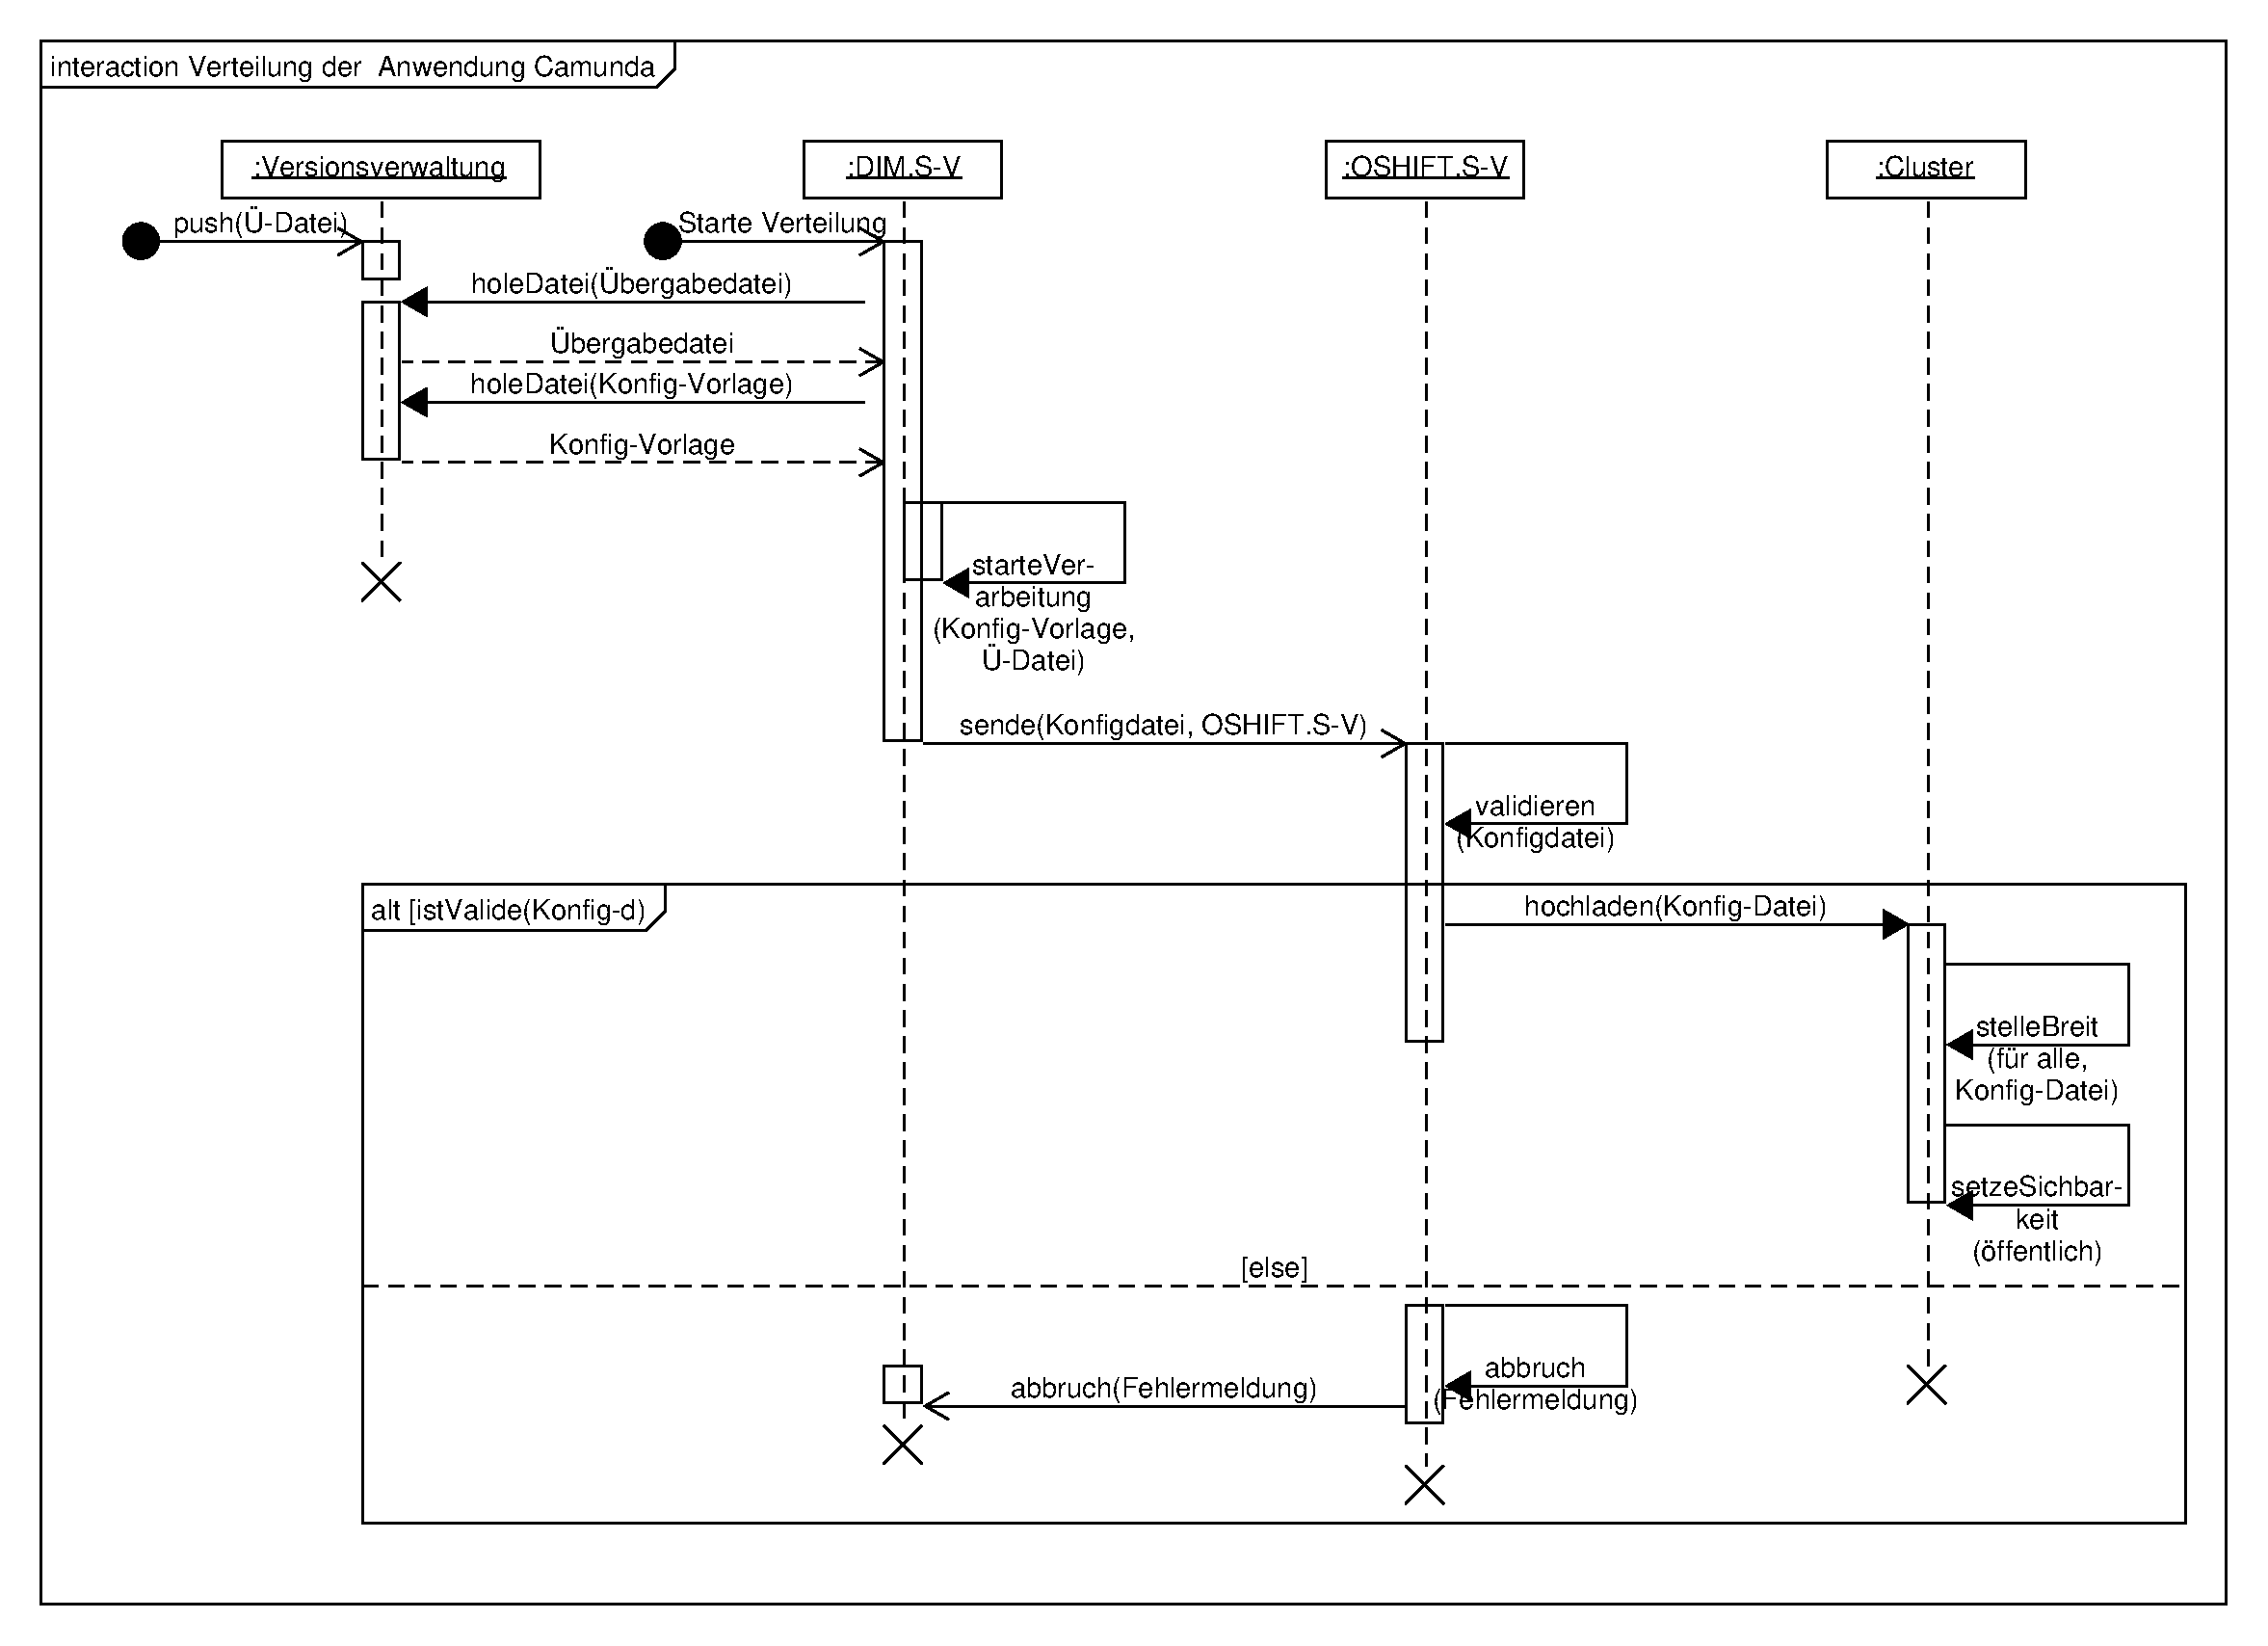
\includegraphics[scale=0.39]{img/prozessDeploymentCamunda.pdf}
	\caption{(adaptiertes) Sequenzdiagramm zur Verteilung der Anwendung \textsc{Camunda}}
	{\footnotesize Quelle: eigene Darstellung \par \textit{unternehmensintern}}
	\label{abb:prozessDeploymentCamunda}
\end{figure}
Die Anforderungen $A_{1}, ..., A_{10}$ wurden auf unterschiedliche Weise in diesem Prozess umgesetzt. $A_{1}$ und $A_{2}$ beziehen sich auf die Konfigurationsdatei und die Übergabedatei. Die Anforderungen wurden durch die Standardisierung der Übergabedatei, die Generierung der Konfigurationsdatei und die Validierung dieser umgesetzt. Die Möglichkeit der Definition von Umgebungsvariablen ist in der Übergabedatei gegeben. Über die Konfigurationsdatei werden die Komponenten verteilt. $A_{3}$ beschreibt die Anforderung, dass konsistente Komponenten verteilt werden. Die Validierung dieser erfolgt durch das \textsc{OpenShift}-Cluster und ist somit gewährleistet. Des Weiteren unterstützt der, in Abbildung \ref{abb:prozessDeploymentCamunda}, dargestellte Prozess die Anforderung $A_{4}$, indem eine Konfigurationsdatei als \enquote{Deployment}-Artefakt verteilt wird. Damit ist der Prozess entkoppelt von dem Inhalt des Containers. Anforderung $A_{5}$ bis $A_{7}$ wird durch die direkte Kommunikation (über die \ac{API}) der Verteilungsanwendung \textsc{Ara} erfüllt. \textsc{Ara} kommuniziert ausschließlich über die \textsc{OpenShift}-\ac{API}. Da diese Verteilungsanwendung automatisch und revisions-konform ist, sind alle verbleibenden Anforderungen erfüllt. Die Funktionalitäten der Methoden, die in Abbildung \ref{abb:prozessDeploymentCamunda} verwendet wurden, werden in der Tabelle \ref{tab:methodenFunktion} kurz beschrieben. Dies dient der Übersichtlichkeit und dem Verständnis. 

\begin{longtable}{@{}p{5.5cm}p{8.0cm}@{}}
	\toprule[1.5pt]
	\textbf{Methode} & \textbf{Beschreibung} \\* \midrule
	\endfirsthead
	%
	\multicolumn{2}{c}%
	{{\bfseries Tabelle \thetable\ von vorheriger Seite fortgeführt.}} \\
	\toprule
	\textbf{Methode} & \textbf{Beschreibung} \\* \midrule
	\endhead
	%
	\bottomrule
	\endfoot
	%
	\endlastfoot
	%
	push(Ü-Datei) & Veröffentlicht die Übergabedatei in der Versionsverwaltung. \\
	holeDatei(Datei) & Lädt die angegebene Datei von der Versionsverwaltung auf einen Server, der die Methode aufgerufen hat. \\
	starteVerteilung(Konfig-Vorlage, Ü-Datei) & Damit wird die Erstellung der angereicherten Konfigurationsdatei gestartet. \\
	sende(Konfig-Datei, Server) & Diese Methode versendet die Konfigurationsdatei an den entsprechend Server. \\
	validieren(Konfig-Datei) & Überprüft die Konfigurationsdatei auf Syntax-Fehler. \\
	hochladen(Konfig-Datei) & Lädt die Datei in \textsc{OpenShift}-Cluster hoch.\\
	stelleBereit(für wen?, Datei) & Diese Methode schaltet die angegebene Datei für alle berechtigten Benutzerinnen auf dem Cluster frei.\\
	setzeSichtbarkeit(Sichtbarkeit) & Veröffentlicht die Komponenten, die durch die Konfigurationsdatei beschrieben wurden. Damit ist der Verteilungsvorgang abgeschlossen.\\
	abbruch(Fehlermeldung) & Bricht den Verteilungsprozess ab und gibt eine Fehlermeldung zurück.\\* \bottomrule
	
	\caption{Überblick über die verwendeten Methoden in Abbildung \vref{abb:prozessDeploymentCamunda}}\label{tab:methodenFunktion}\\
\end{longtable}
 
\section{Ergebnis der Forschungsfrage eins}
Die Ergebnisse der Forschungsfrage eins -- Wie können Container-Anwendungen den Prozess des automatisierten \enquote{Deployments} unterstützen? -- werden nachfolgend kurz zusammengefasst. Eine kritische Betrachtung des gesamten Ergebnisses der Bachelorarbeit ist im Epilog (siehe Kapitel \vref{kritischeBetrachtung}) zu finden.

\paragraph{Prozess wird generisch(er)} Durch die Verwendung dieses Prozess können in Zukunft viele Anwendungen mit nur einem Prozess verteilt werden. Dies ist bedingt durch die Entkopplung der Verteilungslogik und dem eigentlichen Prozess. Da \textsc{OpenShift} nach dem Erhalt der Konfigurationsdatei die wirkliche Verteilung der Komponenten übernimmt, hat sich das komplette Verständnis eines \enquote{Deployments} innerhalb der \ac{SVI} verändert beziehungsweise wird sich verändern. Der neuartige Prozess verteilt nur noch die Konfiguration(-sdatei) und nicht, wie bei den vorherigen Prozessen, den Programmcode oder das Kompilat des Codes. Damit kann der Prozess eine Verteilungsobjekt-unabhängige Logik verwenden. Dieser profitiert von den oben genannten Vorteilen der Container-Anwendungen (vgl. dazu \vref{kap:container}). Des Weiteren profitiert die Endkundin von der ständigen Verfügbarkeit der \enquote{Cloud}, da eine Verteilung einer neuen Version während der Betriebszeiten gemacht werden kann -- dadurch wird eine schnellere \ac{TTM} erreicht. Der, in Abbildung \vref{abb:prozessDeploymentCamunda} abgebildete, Prozess stellt einen ersten Versuch einer automatisierten Verteilung (von Container-Anwendungen) dar. In weiteren Evaluierungen muss der neue Prozess seine Vorteile unter Beweis stellen. Bis dieser von den Verantwortlichen freigegeben wird und produktiv geht, sind noch einige Schritte notwendig, wie z.\,B. die Qualitätssicherung und die Prüfung auf Revisions-Tauglichkeit.

\paragraph{Aufwand ist langfristig geringer} Dieser Teil des Ergebnisses folgt aus der Aussage, dass der Prozess generischer wird: Der anfängliche Aufwand der Entwicklung eines Container-\enquote{Deployment}-Prozesses ist im Unternehmen \ac{SVI} höher, da noch kein Wissen über die Container-/\enquote{Cloud}-Technologie vorhanden war. Des Weiteren gab es kein etabliertes Vorgehen, wie Container-Anwendungen im Bereich der Verteilung behandelt werden. So musste eine Übergabe- und Konfigurationsdatei entwickelt werden, die Infrastruktur (nicht Teil dieser Arbeit) für \textsc{OpenShift} und Container-/\enquote{Cloud}-Produkte geschaffen werden. Außerdem wurden Regeln entwickelt (nicht Teil dieser Arbeit), wie die Zusammenarbeit zwischen den einzelnen, beteiligten Abteilungen funktioniert. Ist der Verteilungsprozess entwickelt und läuft stabil, benötigt dieser keinen weiteren Entwicklungsaufwand. Solange die Anforderungen der Plattform \enquote{OpenShift} nicht verändern, benötigt der Prozess fachlich keine Weiterentwicklung. Somit pendelt sich der Aufwand auf einem konstant niedrigem Niveau ein. Die verbleibenden, aufwand-verursachenden Aufgaben beschränken sich auf die Betreuung im Fehlerfall (Konfigurationsdatei ist fachlich nicht korrekt) und auf die Überwachung der Verteilung neuer Anwendungen. Im Gegensatz dazu stehen die aktuellen Prozesse, die für die Bestandssysteme der \ac{SV} implementiert sind. Hier müssen ständig Anpassungen am Verteilungsprozess gemacht werden, da Kompilate und Quellcode verteilt wird und der \enquote{Deployment}-Prozess auch Kompilierungen vornimmt.
 
\paragraph{Verbesserte Kontrolle des Erfolges} Dies ist bedingt durch die Verteilung einer einzigen Konfigurationsdatei während eines \enquote{Deployments}. Es müssen nicht mehr tausende Artefakte eines Programms verteilt werden. Dadurch ist die Kontrolle des Erfolges beziehungsweise Misserfolges im Vergleich zum jetzigen Prozess einfacher. Im Fehlerfall muss eine Datei, die Konfigurationsdatei, überprüft werden. Die Generierung dieser Datei beschränkt sich auf einen Generierungsalgorithmus, der aus einer Übergabedatei die Konfigurierung ableitet. Wenn dieser getestet ist und fehlerfrei läuft, ist die Fehlerquelle bei einer falschen Verteilung von Komponenten initial beschränkt auf die Übergabedatei. Diese kann einfach kontrolliert und verbessert werden. Es sind immer noch Fehler möglich, jedoch ist die Anzahl der möglichen Fehlerquellen gesunken.

\paragraph{Kritik am Generierungsalgorithmus \ref{algo:configGenerierung}} Dieser Algorithmus \vref{algo:configGenerierung} ist, wie schon erwähnt, bezüglich seiner Laufzeit $T(x)$ und Komplexität $\mathcal{O}$ nicht optimiert. Somit Bedarf dieser noch weiteren Verbesserungen, um die Leistung zu steigern. Problematisch sind die ineinander kombinierten Schleifen, da sie die Laufzeit im schlechtesten Fall polynominell, d.\,h. pro Schleife erhöht sich der (positive) Exponent von $n^{c}$  um eins und damit die Komplexitätsklasse $\mathcal{O}(n^{c}),\,c \ge 1$. Wie oben beschrieben kann über die Vermeidung von ineinander kombinierten Schleifen die Komplexität klein gehalten werden. Eine erste Möglichkeit ist es, das Modul \textsc{PyYaml} zu nutzen, dass durch die Übersetzung der Konfigurationsdatei in ein \ac{K-V}-Objekt Zugriffe der Komplexität $\mathcal{O}(1)$ zulässt. Die Komplexität $\mathcal{O}(1)$ bedeutet übersetzt in diesem Kontext ein direkter Zugriff auf ein Element.

\paragraph{Ausblick: Weitere Evaluierung notwendig} Um die Qualität des Prozesses weiter zu verbessern, sind weitere Schritte notwendig. So müssen die Regeln zur Übergabe der Dateien, zum Aufbau der Konfigurationsdatei und zur Zusammenarbeit erstellt beziehungsweise verbessert werden. Auch müssen Management-Entscheidungen zur Standardisierung dieses Prozess angestoßen und verfolgt werden. Eine weitere Empfehlung ist, den langfristigen Nutzen dieses Prozess zu analysieren, um Verbesserungspotentiale zu finden. Die Forschungsfrage eins versteht sich als ersten Versuch ein lauffähiges Container-\enquote{Deployment} in der \ac{SVI} zu entwickeln -- es sind weitere Schritte bis zum Produktivgang des Prozesses nötig.
\chapter[Forschungsfrage 2]{Welche wirtschaftlichen Vorteile hat der Einsatz von Containern auf den Prozess des automatisierten \enquote{Deployments}?} \label{ff2}
In diesem Kapitel wird die wirtschaftliche Komponente des \enquote{Deployment}-Prozesses beleuchtet, wobei der Geschäftsprozess \enquote{Release} und der \enquote{Business Case} \enquote{\enquote{Deployment} einer Container-Anwendung}  betrachtet werden. Zuerst werden die Grundlagen der beiden Teilbereiche beschrieben, um später diese für die Prozessanalyse und den Soll-Ist-Vergleich der Nutzung der \enquote{Business Case}-Methodik zu verwenden. Das Kapitel schließt mit einem Teilergebnis der Forschungsfrage zwei ab.

\section{Grundlagen: Definition der Begrifflichkeiten zur Forschungsfrage zwei}
Dieses Teilkapitel soll grundlegende Begrifflichkeiten, die im weiteren Verlauf dieser Arbeit verwendet werden, definieren, um so eine einheitliche Terminologie der Begriffe zu entwickeln. Dadurch wird ein gemeinsames Verständnis erzeugt.

\paragraph{Geschäftsprozessanalyse}
Der Begriff \enquote{Geschäftsprozess} beschreibt eine zusammenhängende Folge von Aufgaben beziehungsweise Tätigkeiten, die in einem Unternehmen wiederkehrend abgeschlossen werden, um die Unternehmens- und Organisationsziele zu erreichen. Die Analyse untersucht schlussendlich dieselben Sachverhalte wie auch die klassischen Ansätze der Organisationslehre. \autocite[vgl.][S.\,5]{staud_geschaftsprozessanalyse_2006} Diese sind die Effizienzsteigerung und die Einsparung. Dabei werden die zu leistenden Tätigkeiten, Aufgaben und Arbeitsabläufe auf die genannten Ansätze optimiert. Im Vergleich zur klassischen Optimierung steht bei der Geschäftsprozessanalyse eine andere Perspektive im Fokus. Hier werden die \enquote{längere(n) zusammenhängende(n) Folgen von Tätigkeiten, die zur Erledigung einer größeren Aufgabe nötig sind}\autocite[][S.\,5]{staud_geschaftsprozessanalyse_2006}, betrachtet. Damit ist der gesamte Ablauf eines Prozesses als Ausgangspunkt der Analyse zu betrachten und nicht mehr nur einzelne Tätigkeiten und Stellen.
\par 
Um das weitere Verständnis der Begrifflichkeiten zu fördern, werden folgende definiert\autocite[vgl.][S.\,4-5]{staud_geschaftsprozessanalyse_2006}: Aufgaben und deren Eigenschaften, Aufgabenfolgen und Funktionen. Aufgaben sind Teilarbeitspakete einer Tätigkeit, die auf unterschiedlichen Ebenen betrachtet werden können. Die kleinste Einheit einer Aufgabe ist die Elementaraufgabe, die nicht weiter teilbar ist. Wichtig ist, dass Aufgaben teilbar und wieder zusammenfassbar sind. Dadurch wird eine unterschiedliche Aggregationsstufe erreicht. Das Problem der Aggregation ist, dass die Modelliererin, geprägt durch ihre Wahrnehmung, die Ebene der Betrachtung einer Aufgabe bzw. Tätigkeit subjektiviert und so das Ergebnis stark beeinflusst wird -- so auch die Länge der Geschäftsprozesse. Die sequenzielle Folge von Aufgaben entsteht durch die Erstellung eines Vorgangs, der eine Abfolge von Tätigkeiten zur Realisierung von Aufgaben beschreibt. Schließlich wird ein Geschäftsprozess von \cite{staud_geschaftsprozessanalyse_2006} definiert als: \enquote{[...] besteht aus einer zusammenhängenden abgeschlossenen Folge von Tätigkeiten, die zur Erfüllung einer betrieblichen Aufgabe notwendig sind. Die Tätigkeiten werden von Aufgabenträgern in organisatorischen Einheiten unter Nutzung der benötigten Produktionsfaktoren geleistet. Unterstützt wird die Abwicklung der Geschäftsprozesse durch das Informations- und Kommunikationssystem IKS des Unternehmens.}\autocite[][S.\,9]{staud_geschaftsprozessanalyse_2006} Eine weitere Definition charakterisiert den Geschäftsprozess als \enquote{[...] eine zielgerichtete, zeitlich logische Abfolge von Aufgaben, die arbeitsteilig von mehreren Organisationen oder Organisationseinheiten unter Nutzung von Informations- und Kommunikationstechnologien ausgeführt werden können. Er dient der Erstellung von Leistungen entsprechend den vorgegebenen, aus der Unternehmensstrategie abgeleiteten Prozesszielen. Ein Geschäftsprozess kann formal auf unterschiedlichen Detaillierungsebenen und aus mehreren Sichten beschrieben werden.}\autocite[][S.\,41]{gadatsch_grundkurs_2010} Die zweite Definition wird in dieser Arbeit verwendet, denn sie stellt die Unternehmensstrategie als zentralen Messfaktor in den Mittelpunkt. Werden alle Geschäftsprozesse linear kombiniert, entsteht die Darstellung der Wertschöpfungskette eines Unternehmens. Deswegen gibt es nur systemrelevante Geschäftsprozesse in einem Unternehmen. Sie können noch Optimierungspotenzial enthalten. Ein Geschäftsprozess wird am Kunden orientiert. Es wird zwischen Kern- und unterstützenden Prozessen unterschieden: Bei Kernprozessen handelt es sich um die Hauptleistung eines Unternehmens, wie die Produktion eines Autos bei einem Autohersteller. Die Unterteilung in Kern- und unterstützende Prozesse beschreibt dabei nicht die Wichtigkeit dieser; es ist also keine Einteilung in weniger wichtig und wichtig vorzunehmen.\autocite[vgl.][S.\,11]{staud_geschaftsprozessanalyse_2006} \par

Geschäftsprozesse haben verschiedene Eigenschaften, wie der Automatisierungsgrad, die Datenintegration und die Prozessintegration. Der Automatisierungsgrad beschreibt, wie groß der Anteil der Aufgabenerfüllung ist, welcher dunkel, d.\,h. ohne menschliche Interaktion, bewältigt werden kann. Die Datenintegration ist ein wichtiger Bestandteil bei Optimierungsvorhaben, denn sie sollte bei 100 Prozent liegen, um Inkonsistenzen der Daten auszuschließen. Bei weniger als 100 Prozent entwickeln sich Parallelwelten im Unternehmen. Ist ein Geschäftsprozess über viele verschiedene traditionelle Organisationsbereiche aufgespannt, so ist seine Prozessintegration hoch. Gibt es Organisationsbrüche, d.\,h., wird ein Prozess aktiv an einer beteiligten Abteilung vorbeigeführt, muss die Notwendigkeit dieser Maßnahme bei der Optimierung überprüft werden. Zu den Komponenten der Geschäftsobjekte: Je nach Ziel der Untersuchung können viele Komponenten beteiligt sein und können damit identifiziert werden. Die \ac{BWL} beschränkt diese auf die formellen Strukturen einer Organisation und auf das Handeln der Beteiligten, das unmittelbar Einfluss auf den Geschäftsprozess hat.\autocite[vgl.][S.\,15]{staud_geschaftsprozessanalyse_2006} \par

Ziel der Geschäftsprozessanalyse ist es, eine Ist-Analyse des Prozesses durchzuführen, um so eine Bestandsaufnahme vorhalten zu können, und eine Optimierung des Prozesses, die die Beseitigung von Schwachstellen zur Folge hat. Diese Schwachstellen werden bei der Ist-Analyse entdeckt. Einschränkend zu erwähnen ist, dass die Methodik der Geschäftsprozessanalyse nicht genau definiert ist, da die Identifikation (Detaillierungsgrad) und Abgrenzung (Länge) der Prozesse subjektiv beeinflusst werden. Das Modell der \ac{EPK} ist eine mögliche Methodik, um Geschäftsprozesse zu analysieren und zu beschreiben.\autocite[vgl.][S.\,59]{staud_geschaftsprozessanalyse_2006} \ac{EPK} ist ein Vorgehensmodell zur Sichten-orientierten Modellierung von Geschäftsprozessen, bei dem ein Prozess und seine dazugehörenden Funktionen in einer zeitlich-logischen Abfolge illustriert werden.\autocite[vgl.][S.\,4]{scheer_objektorientierte_1997} Die Kontrollflusssteuerung zwischen den einzelnen Funktionen eines Geschäftsprozesses werden über Geschäftsregeln gesteuert. Diese beinhalten folgende Konstrukte: Ereignis, Bedingung und Funktion/Methode/Aktion. Entscheidungen werden über die verfügbaren Verknüpfungsfunktionen modelliert:\autocite[vgl.][S.\,4]{scheer_objektorientierte_1997} \textit{AND}-, \textit{OR}- und \textit{XOR}-Verknüpfung\footnote{Hier wird an die gängige Schreibweise der Logikgatter angeknüpft.}. Des Weiteren gibt es eine andere Methodik, die in einem Standard, \ac{BPMN} Version 2.0 \autocite{object_management_group_omg_business_2011}, definiert ist, der Geschäftsprozesse modelliert. Außerdem wurde dieser Standard in der Norm ISO/IEC 19510 verankert.\autocite{ict1_information_2020} Im Gegensatz zur \ac{EPK} fokussiert sich \ac{BPMN} rein auf die Modellierung eines Prozesses und nicht auf folgende Strukturen: Prozesslandschaft, Aufbauorganisation, Daten, Strategie, Geschäftsregeln und IT-Landschaft.\autocite[vgl.][S.\,28]{freund_praxishandbuch_2017} Es gibt eine Software-Lösung für \ac{BPMN}, die in der \ac{SVI} eingesetzt wird und später die erste Container-Applikation für den neuen \enquote{Deployment}-Prozess ist.

\paragraph{\enquote{Business Case}}\label{sec:businessCase}
In diesem Teilkapitel werden der Aufbau eines Geschäftsszenarios und die grundsätzliche Methodik erläutert, da eine tiefgreifende, ausführliche Beschreibung des gesamten Themenkomplexes den Rahmen dieser Arbeit überschreitet: Eine vollumfängliche Betrachtung eines \enquote{Business Case} kann eine eigene Bachelor-Thesis darstellen. \par
Die Erstellung eines Geschäftsvorfalls (engl. \enquote{business case}) ist für das Unternehmen bei der Betrachtung eines Projekts von elementarer Bedeutung. Ohne dessen Erstellung könnten folgende Probleme mit hoher Wahrscheinlichkeit auftreten\autocite[][S.\,4]{herman_is_2009}: 
\begin{itemize}
	\item \enquote{The organization wastes valuable resources on projects that don't help the organization achieve its objectives. This leaves fewer resources available for more valuable projects.
	\item The organization has no clear basis to prioritize projects, for establishing what is important. Without a Business Case--and some organization-wide agreed measure of “value”--there is no	means of determining which projects are important, and which are less so.
	\item There is likely to be disappointment after the completion of the
	project, as the stakeholders wonder why the project is not giving the great results they imagined [...].
	\item No target is established for why the project's deliverables are
	being created--other than the meeting of technical specifications.
	\item The organization has no opportunity to improve its project management maturity. One key learning from each project should be: “how well did the resource usage support the organization's goals?”}
\end{itemize}
Grundsätzlich ist ein Geschäftsszenario eine betriebswirtschaftliche Beurteilung einer Investition. Dabei werden deren Kosten und Nutzen nach einer zuvor definierten Methodik gemessen, beurteilt und dokumentiert. Am Ende eines \enquote{Business Case} entsteht eine mit Informationen begründete Aussage über die Rentabilität der Investition. Das Geschäftsszenario soll für jedes Projekt eines Unternehmens erstellt werden. Dabei soll mit diesem der Mitteleinsatz gegenüber den Führungskräften beziehungsweise der Geschäftsführung gerechtfertigt werden. Bestandteile des \enquote{Business Case} sind somit rein monetäre Größen und nicht-monetäre Aspekte (meist Abwägungen \enquote{hinsichtlich Risikoadressierung und Strategieorientierung in Verbindung mit den jeweiligen Optionen und deren wirtschaftlicher Vorteilhaftigkeit}\autocite[][S.\,12]{brugger_it_2009}). Es entsteht eine ganzheitliche Dokumentation aller entscheidungsrelevanter Sachverhalte: \enquote{Ein Business Case fasst alle entscheidungsrelevanten Aspekte eines geplanten Vorhabens mit dem Ziel zusammen, die wirtschaftliche Vorteilhaftigkeit und strategische Konformität des Gesamtprojekts aufzuzeigen und eine abschließende Management-Entscheidung über dessen Ausführung zu ermöglichen.}\autocite[][S.\,13]{brugger_it_2009} Abzugrenzen ist dieser Begriff von dem \enquote{Business Plan}: Er basiert auf der Gesamtbetrachtung einer organisatorischen Einheit bis zur Ebene des Gesamtunternehmens. Der \enquote{Business Plan} erstellt ein Gesamtbild und ist nicht auf einzelne Projekte und Investitionsentscheidungen fokussiert. 
\par
Im Bereich der Investitionen gibt es zwei Entscheidungspfade: die Durchführungsentscheidung (absolute Vorteilhaftigkeit) und die Auswahlentscheidung (relative Vorteilhaftigkeit).\autocite[vgl.][S.\,14]{brugger_it_2009} Die Differenzierung beider Möglichkeiten ist durch die Menge an zu bewertender Investition gegeben: Bei einer Investition werden die absolute (Ist diese wirtschaftlich?) und bei mehreren die relative Vorteilhaftigkeit (Welche ist wirtschaftlicher?) bewertet. Die Grundannahme der Investitionen lautet immer: Der Nutzen muss größer sein als die Kosten. Wenn die Kosten den Nutzen übersteigen, gibt es drei Bewertungsmöglichkeiten. Die Investition is entweder aussichtsreich oder aussichtslos, doch andere Gründe sprechen dafür, oder aussichtslos. Aussichtsreiche Projekte sollten an die Erkenntnisse des Geschäftsszenarios angepasst werden. Aussichtslose Projekte mit anderen Gründen müssen genauestens untersucht werden, um eine Entscheidung über die Realisation des Projekts zu treffen. Aussichtslose Projekte werden abgelehnt. Um den Nutzen der Erstellung eines \enquote{Business Case} zu unterstreichen, sind folgende Vorteile zu nennen: Er erhöht erstens die Entscheidungssicherheit; schafft zweitens Entscheidungsspielraum, Übersicht und Transparenz, Verbindlichkeit, Klarheit, Nachvollziehbarkeit und Vergleichbarkeit; er unterstützt drittens die \enquote{Controlling}-Division.\autocite[vgl.][S.\,17]{brugger_it_2009} \par
Mit dem \enquote{Business Case} kann die Informatik ihren Wertschöpfungsbeitrag am Unternehmen beweisen. Aus der Überlegung heraus, die Informatik eines Unternehmens effektiv und effizient zu gestalten, ist die Betrachtung eines Geschäftsszenarios von großer Bedeutung. Die Einordnung des Unternehmenszweckes ist bei der Erstellung des \enquote{Business Case} wichtig. Die Informatik kann auf zwei Arten dem Unternehmenszweck dienen: Sie generiert Wert (\enquote{value creation}) oder sie beschützt Wert (\enquote{value protection}). So hat die Art des Dienstes direkte Auswirkungen auf den \enquote{Business Case}-Fokus. Bei der Wertsicherung wird ein Kostenvergleich in der Wirtschaftlichkeitsanalyse durchgeführt; die Wertgenerierung hingegen bedingt einen Kosten-Nutzen-Vergleich. Die Wertsicherung ist aus Sicht der Informatik für ein Unternehmen eine zwingende Aktivität. Problematisch ist es, da die Kunden (meist intern) keinen unmittelbaren Wertschöpfungscharakter erkennen und deswegen diese Maßnahmen meist nicht hoch priorisiert sind, jedoch erheblichen Einfluss auf die Geschäftstätigkeit eines Unternehmens haben.\autocite[vgl.][S.\,27]{brugger_it_2009} Im Anhang \vref{abb:entscheidungBC} ist ein stark vereinfachtes Flussdiagramm dargestellt, das die Entscheidungspfade für und gegen die Erstellung eines Geschäftsszenarios illustriert. Dieses kann benutzt werden, um eine schnelle Entscheidung zu erhalten, dennoch ist der eigentliche Prozess komplizierter -- wie in der Abbildung \vref{abb:entscheidungBC} dargestellt. Beeinflusst wird dieser nicht nur durch staatliche Verordnungen und Gesetze, sondern auch durch innerbetriebliche Vorschriften. 
\par
Ein \enquote{Business Case} kann intern oder extern erstellt werden. Es sind noch weitere Kombinationsmöglichkeiten denkbar, die in der Praxis jedoch kaum eine Rolle spielen.\autocite[vgl.][S.\,33]{brugger_it_2009} Es gibt für beide Möglichkeiten, intern oder extern erstellt, Vor- und Nachteile, die im Anhang \vref{appendixVorNachteileErstellungBC} abgebildet sind. Die beteiligten Einheiten des Unternehmens entstammen der Informatik, einer \enquote{Business Unit}, der Finanzabteilung (meist \enquote{Controlling}) und der Personalabteilung. Entscheidungen, die das Projekt und somit das Geschäftsszenario betreffen, werden durch die höheren Führungsebenen in Verbindung mit den projektanfordernden Bereichen getroffen. Die Erstellung teilt sich in drei Ebenen auf: Initialisierung (\enquote{Business Case Definition}), Entwicklung (\enquote{Business Case Development}) und Prüfung (\enquote{Business Case Quality Check}).\autocite[vgl.][S.\,41-42]{brugger_it_2009} Während der Initialisierungsphase werden die Teams definiert, eine Eingrenzung der beteiligten Abteilungen vereinbart, die Kriterien bzw. Parameter für die Wirtschaftlichkeitsrechnung festgelegt und die Kalkulationsmethoden für die Ermittlung der Kennzahlen gewählt. In der Entwicklungsphase werden folgende Arbeitsschritte durchgeführt: Projektplanung/Systemkonzeption, Erhebung und Analyse der Kosten/des Nutzens, Aufbau des Wirtschaftlichkeitsmodells sowie Auswertung der Ergebnisse, die eine Sensitivitäts- (Versuch, die optimale Lösung weiter zu verbessern), eine Risiko- und eine Strategieanalyse enthält und die Zusammenfassung für die Führungsebene. Im Anhang \vref{abb:entwicklungBC} ist eine Abbildung mit der chronologischen Anordnung der Arbeitsschritte zu sehen, die nochmals auf die Abhängigkeit der Schritte hinweist. Die letzte Phase beschäftigt sich mit der Qualitätssicherung der gewonnenen Erkenntnisse, bei der eine Validierung der Annahmen, die Prüfung der eingegebenen Daten und eine Abstimmung mit anderen Projekten durchgeführt werden. 

\section{Geschäftsprozess: \enquote{Release} von neuen Anwendungsversionen}
Der Geschäftsprozess \enquote{Release} beinhaltet den \enquote{Deployment}-Prozess, deswegen wird in der Geschäftsprozessanalyse der \enquote{Release}-Prozess als Ganzes betrachtet, um den wirtschaftlichen Effekt der Veränderung des \enquote{Deployments} zu untersuchen. Es wird zuerst der aktuelle \enquote{Release}-Prozess  ohne den Container-\enquote{Deployment}-Prozess betrachtet.
\par
Der aktuelle \enquote{Release}-Prozess folgt in den Entwicklungsarbeiten dem Vorgehensmodell \enquote{Wasserfall}. Dies ist ein iteratives Vorgehensmodell zur Anwendungsentwicklung, das sich streng Modell in Konzeption und Umsetzung auf teilt.\autocite[vgl.][S.\,24]{freund_praxishandbuch_2017} Die \ac{SVI} hat ein Meilenstein-Konzept für das \enquote{Release} entwickelt, das das genaue Vorgehen dieses Geschäftsvorfalls beschreibt. Dieser definiert Aufgaben und Tätigkeiten, die zu einer Folge kombiniert werden. 

\begin{figure}[h!]
	\centering
	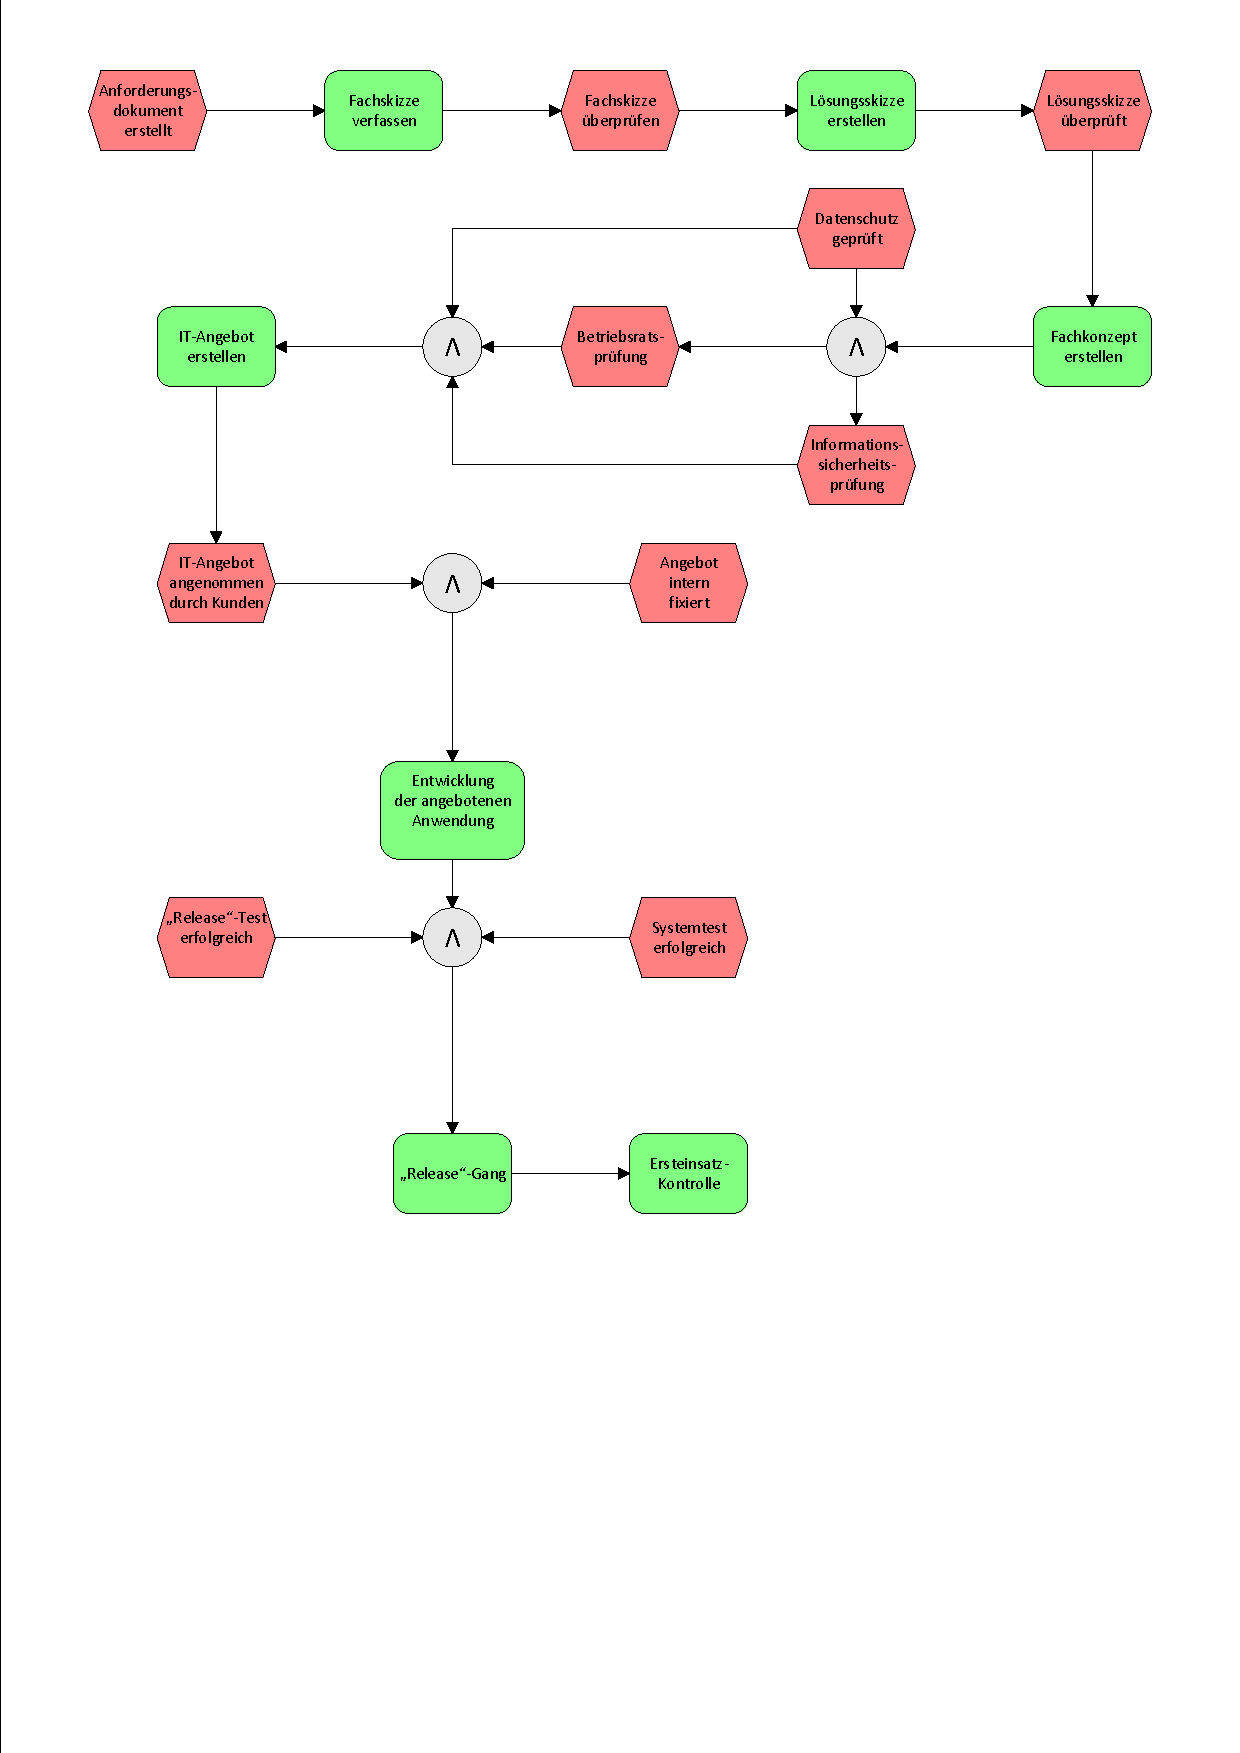
\includegraphics[scale=0.51]{img/prozessRelease.pdf}
	\caption{\acs{EPK} zum Geschäftsvorfall \enquote{Release}}
	\label{abb:meilensteineRelease}
	{\footnotesize Quelle: in Anlehnung an unternehmensinterne Dokumente}
	{\footnotesize \par \textit{unternehmensintern}}
\end{figure}

Die Abbildung \vref{abb:meilensteineRelease} zeigt die abgewandelte \ac{EPK} des Geschäftsprozesses: Die rot gefärbten Formen sind Ereignisse, die grünen Funktionen bzw. Arbeitspakete und das grau gefärbte Symbol beschreibt eine logische \enquote{AND}-Verknüpfung. Dieser Prozess hat verschiedene Prüfstellen, die die Qualität der erstellten Dokumente überprüfen. Erst ab der Funktion \enquote{Entwicklung der angebotenen Anwendung} werden Anwendungen programmiert. Davor sind alle Aktivitäten zur Erstellung, Prüfung und Dokumentation der zu entwickelnden Anwendung durchzuführen. Diese sind mit erheblichen Aufwand verbunden: So muss die Kundin zusammen mit den Kundenmanagerinnen ein erstes Konzept entwickeln und beschreiben was das \enquote{statement of needs} ist. Dieses wird in den nächsten Schritten zu einem Anforderungsdokument überarbeitet, wobei auch mögliche Lösungsvorschläge berücksichtigt werden. Schließlich sind das Fachkonzept und die Lösungsskizze erstellt. Die Kundenmanagerin kreiert ein IT-Angebot, welcher der Kundin vorgelegt wird. Diese beiden Personenkreise verhandeln dann über Kosten und Nutzen des Vorhabens. Sobald die Kundin zustimmt und alle anderen Zustimmungen (Betriebsrat, IT-Sicherheit und Datenschutz) eingeholt sind, startet die Entwicklung der beschriebenen Funktion. Nun folgen Tests in verschiedenen Umgebungen und dann die Freigabe für die Produktivsetzung der neuen Funktion/Anwendung. Danach prüft die Kundin, ob alle vorgesehenen Funktionen nach ihren Vorstellungen umgesetzt wurden. Dieses Vorgehen spiegelt einen linearen Vorgang wider, der sich schwer an sich ständig verändernde Anforderungen anpassen kann. Ist das Fachkonzept freigegeben, kann an diesem nichts mehr geändert werden. Jedoch verändern sich die Anforderungen immer schneller und die Software hat einen immer kürzer andauernden Lebenszyklus innerhalb der \ac{SV}. Die Digitalisierung wird in der \ac{SV}-Strategie als zentraler Bestandteil beschrieben.\autocite[vgl.][]{sv_sparkassenversicherung_sv_2019} Somit wird die Forderung nach einer Anpassung des \enquote{Release}-Prozesses immer stärker.
\par
Durch die Veränderung des \enquote{Deployment}-Prozesses ändert sich der gesamte \enquote{Release}-Prozess ebenfalls: So müssen die Planung und die Nicht-Anpassbarkeit des Fachkonzeptes überdacht werden. Außerdem ist der aktuelle Prozess, wie in Abbildung \vref{abb:meilensteineRelease} dargestellt, so mit den starren Regeln nicht mehr möglich. In einer Übergangsphase, bis ein neuer Geschäftsprozess entwickelt wurde, kann dieser aktuelle in einer abgewandelten Form benutzt werden. Diese Form müsste eine Änderung der Anforderungen und somit eine Änderung des Fachkonzeptes während der Entwicklung neuer Anwendungen zulassen. Dies kann zu inkonsistenten Daten in der Dokumentation führen und ist deswegen mit Vorsicht zu betrachten. Des Weiteren könnte eine Art Kategorisierung für die Anforderungen gemacht werden, d.\,h., zwingend umzusetzende Anforderungen der Anwendungen wären ersichtlich. So könnten die Fachkonzepte in mindestens zu erfüllende und optimale Anteile unterteilt werden. 
\par
Die Container-Anwendungen unterstützen die Schnelligkeit der Entwicklung, da sie direkt mit einem entsprechenden \enquote{Deployment}-Prozess produktiv gehen können. Ist die Teststruktur automatisiert und die Dokumentationspflicht erfüllt, können der Aufwand und damit die Kosten für die Entwicklung einer Funktion einer Anwendung beziehungsweise die Entwicklung einer kompletten Anwendung reduziert werden. Dies folgt aus der Tatsache, dass weniger Arbeitsstunden in die Betreuung, Entwicklung, Kontrolle und Dokumentation investiert werden müssen. Bleibt der Preis der Anwendung gleich, erhöht sich trotzdem der erzielte Gewinn, da die Kosten sich reduzieren. Natürlich sind initial die Kosten höher, da die Entwicklung eines neuen Prozesses sehr viel Aufwand darstellt.
\par
Momentan ist die \ac{SVI} in einer Übergangsphase, in der sie den Geschäftsprozess \vref{abb:meilensteineRelease} weiterhin nutzt. Jedoch wurden hier die oben genannten Veränderungen implementiert. Die illustrierte Weiterentwicklung des \enquote{Deployment}-Prozesses (siehe Kapitel \vref{ff1}) ist eine Möglichkeit, die Kosten durch Reduzierung des Betreuungsaufwandes in der Abteilung \ac{IE2} zu senken.

\section{\enquote{Business Case}: \enquote{Deployment} einer Container-Anwendung}
Die \ac{SV} möchte verschiedene Prozesse dunkel verarbeiten, d.\,h., es soll keine Sachbearbeiterin Arbeit mit der Erledigung dieser haben. Die Prozesse, die unter dem Namen \enquote{Meine \ac{SV}-Online Services} bekannt sind, sind auf der Webseite der \ac{SV}\footnote{unter \href{https://www.sparkassenversicherung.de/content/privatkunden/service/daten/index.html}{\enquote{Meine \ac{SV}-Online Services}} (https://www.sparkassenversicherung.de/content/ privatkunden/ service/daten/index.html)} zu finden. Dort können Kundinnen verschiedene Aufträge selbst durchführen, wie eine Rechnungs-/Policenkopie anfordern, ihre persönlichen Daten ändern, einen Schaden melden, eine bestehende Kfz-Haftpflichtversicherung anpassen und eine privat Haftpflicht- bzw. Hausratversicherung abschließen. Diese Prozesse sollten mittels \ac{BPMN} abgebildet werden. Ein \enquote{statement of needs} der \ac{SV} ist es, diese Prozesse selbstständig zu entwickeln. Durch diesen Wunsch entwickelte die \ac{SVI} in Zusammenarbeit mit der \ac{SV} eine Lösung. Es wurde ein Produktvergleich verschiedener Software-Hersteller durchgeführt. Schließlich hat sich die \ac{SV} in Zusammenarbeit mit der \ac{SVI} für die Software \textsc{Camunda} entschieden. Der Beschaffungsprozess wurde prozess-konform durchgeführt und die Entwicklungsarbeiten im Projektteam begannen. Die Anforderungen der Software \textsc{Camunda} beschrieben u.\,a., dass eine Container-Umgebung für die Verteilung dieser benötigt wird. Das Problem ist, dass dies  bei der Entscheidung zum Kauf der Software nicht berücksichtigt worden war. Daraus resultiert die Anforderung, dass das \enquote{Deployment}-Team eine Lösung für die Verteilung von Container- und damit von \textsc{Camunda}-basierten Anwendungen erforscht und implementiert. Daraus folgt ein gemeinsames Projekt der Infrastruktur- und Betriebsabteilungen der \ac{SVI}: Hier soll ein Software-Produkt gefunden werden, das Revisions-konform und betriebstauglich ist. Die Kriterien der Revision werden von der \ac{BaFin} sowie durch juristische Vorschriften und Gesetze bestimmt. Die Betriebstauglichkeit wird durch Anforderungen der jeweiligen Abteilungen beschrieben. Aus diesen Kriterien folgen Akzeptanzbestimmungen für das Software-Produkt, wie z.\,B. die Multi-Mandanten-Fähigkeit, die Integrationsbereitschaft zu \enquote{Cloud}-Plattformen (\textsc{Amazon Webservices}, \textsc{Microsoft Azure}), die Isolationsfähigkeit der kompletten Plattform im Rechenzentrum, Verschlüsselung der Kommunikation und weitere. Mit Hilfe dieser Anforderungen kann ein Produktvergleich durchgeführt werden zwischen den Lösungen von \textsc{Red Hat} (\textsc{OpenShift}) und \textsc{SuSe} (\textsc{CaaS}). Die Ergebnisse zeigten, dass der Hersteller \textsc{SuSe} zwei Produkte braucht, um die gegebenen Anforderungen zu erreichen. Im Gegensatz dazu erreicht \textsc{Red Hat} mit einem Produkt, \textsc{OpenShift}, alle Anforderungen der \ac{SVI}. Bei Betrachtung der zwei Produktlösungen sind keine nennenswerten Unterschiede zu erkennen. Die beiden Lösungen unterscheiden sich in den Kosten und, dass \textsc{SuSe} zwei Produkte für die Lösung benötigt. Die Kosten sind nachfolgend in der Tabelle \vref{tab:kostenvergleichProdukte} dargestellt. Schließlich wurde bedingt durch die lange Markterfahrung und die Nutzung durch andere Versicherungskonzerne die Lösung von \textsc{Red Hat} eingekauft. Die Lizenzkosten sind unter gewissen Annahmen getroffen, wie die Preise sind Listenpreise, die Berechnungsbasis sind \enquote{Cores} in einer Virtualisierungsumgebung u.\,Ä. Weitere Rechenzentrum-spezifische Details, wie die Ausstattung der Virtualisierungsserver und das Ausfallsicherungskonzept der \ac{SVI}, sind dementsprechend auch Annahmen zur Berechnung der Lizenzkosten.

\begin{table*}[h!]
	\centering
	\ra{1.3} %more space beetween rules
	
	\begin{tabular}{@{}lll@{}}\toprule[1.5pt]
		
		\textbf{Produkt} & \textbf{\enquote{Support}-Plan} & \textbf{Kosten} \\ \midrule
		% below rules with content
		\textsc{OpenShift} & Standard & 80 \enquote{Cores} $\widehat{=}$  86.400\,\euro \\
		& & 160 \enquote{Cores} $\widehat{=}$  172.800\,\euro \\
		
		\textsc{CaaS}\&\textsc{CaP} & Standard & 80 \enquote{Cores} $\widehat{=}$  80.000\,\euro \\
		& & 80 \enquote{Cores} $\widehat{=}$  160.000\,\euro \\
		
		\textsc{OpenShift} & Premium & 80 \enquote{Cores} $\widehat{=}$  128.000\,\euro \\
		& & 160 \enquote{Cores} $\widehat{=}$  256.000\,\euro \\
		
		\textsc{CaaS}\&\textsc{CaP} & Premium & 80 \enquote{Cores} $\widehat{=}$  111.200\,\euro \\
		& & 80 \enquote{Cores} $\widehat{=}$  222.400\,\euro \\		
		
		\bottomrule[1.5pt]
	\end{tabular}
	
	\caption{Vergleich der jährlichen Lizenzkosten}
	\label{tab:kostenvergleichProdukte}
	
\end{table*}
Durch Entscheidung der betreffenden Führungskräfte in Zusammenarbeit mit den Projektbeteiligten wird das Produkt \textsc{OpenShift} der Produktlösung von \textsc{SuSe} bevorzugt. Auch wenn, die Lizenzkosten und der initiale Einführungsaufwand höher sind als bei der \textsc{SuSe}-Lösung. Gemäß des oben genannten Vorgehens eines \enquote{Business Case} (vgl. dazu Kapitel \vref{sec:businessCase}), muss bei einer Investition der Nutzen immer größer sein als die Kosten. Wenn das nicht gegeben ist, muss eine Abwägung getroffen werden, ob es trotzdem wirtschaftlich sinnvoll ist diese Investition zu tätigen. Hier sind die Akzeptanzkriterien nochmals zu überprüfen: \textsc{Red Hat} \textsc{OpenShift} ist bei der \ac{VKB} im Einsatz, die \ac{PNW} führt diese Anwendung aktuelle ein. Somit haben zwei andere öffentlich-rechtliche Versicherer diese Software im Einsatz. Auch die lange Markterfahrung von \textsc{Red Hat} im Bereich Finanzen und Automatisation sprechen für diesen Konzern. Im Gegensatz dazu ist die Produktlösung von \textsc{SuSe} noch nicht lange auf dem Markt (seit Herbst 2017) und die Lösung besteht zwei Produkten. Die Container-Anwendungen werden auf der Plattform \textsc{OpenShift} von \textsc{Red Hat} betrieben.
\par
Die vollständige \enquote{Business Case}-Analyse wird teilweise durch die Projektkontrollgremien implementiert, so wird ein Kosten-Nutzen-Vergleich und eine Investitionsrechnungen durchgeführt. Jedoch wurde das Vorgehen auf die \ac{SVI} adaptiert. Dies ist der Unternehmensstruktur der \ac{SV} geschuldet: Die \ac{SV} ist unterteilt in sogenannte Ressorts. Die \ac{SVI} als Informatik-Dienstleitserin und vollständige Tochtergesellschaft ist dem Ressort drei \enquote{\textit{Leben/IT}} unter Dr.~Wittmann zugeordnet. Damit sind viele Tätigkeiten im \enquote{Controlling} Aufgabe der \ac{SV}, so auch die Verantwortung, wie Entscheidungen getroffen werden. 

\section{Ergebnis der Forschungsfrage zwei}
Die Ergebnisse der Forschungsfrage zwei -- Welche wirtschaftlichen Vorteile hat der Einsatz von Container auf den Prozess des automatisierten \enquote{Deployments}? -- werden nachfolgend kurz zusammengefasst. Eine kritische Betrachtung des gesamten Ergebnisses der Bachelorarbeit ist im Epilog (siehe Kapitel \vref{kritischeBetrachtung}) zu finden.

\paragraph{\enquote{Business Case}-Methodik} Die Methodik des \enquote{Business Case} konnte aus verschiedenen Gründen nicht komplett umgesetzt werden: So sind nicht genug Daten zur finanziellen Bewertung von \textsc{Camunda} und einen Vergleichsprodukt vorhanden. Die Forderung Container-Anwendungen einzusetzen ist keine bewusste Entscheidung gewesen, sondern eine Konsequenz aus dem Einkauf der Software \textsc{Camunda} -- gewissermaßen eine Nebenbindung, um diese einsetzen zu können. Aus dieser Nebenbedingung entstand die Anforderung eine Plattform für den Betrieb von Container-Anwendungen bereitzustellen. Mit dieser Anforderung ist die Frage nach der wirtschaftlichen Sinnhaftigkeit von Container-Anwendung und deren Verteilung nicht zu stellen, sondern es ist eine wirtschaftlich sinnvolles (durch Akzeptanzkriterien messbares) Software-Produkt zu suchen. Dabei ist der Produktvergleich eine akzeptierte Methode. Das Vorgehen des Produktvergleichs wurde über Anforderungen messbar gestaltet. Dieser Produktvergleich ist jedoch nicht Teil dieser Arbeit. Abschließend ist der \enquote{Business Case} und damit die Forschungsfrage eins \enquote{Welche wirtschaftlichen Vorteile hat der Einsatz von Container auf den Prozess des automatisierten \enquote{Deployments}?} nicht durch die oben genannte Methodik aufgrund der Datenlage der \ac{SV} beziehungsweise \ac{SVI} beantwortbar. Jedoch kann eine generelle Aussage getroffen werden (vgl. Kapitel \vref{sec:auswirkungCA} Wirtschaftliche Auswirkungen).

\paragraph{Auswirkungen der Entscheidung der \ac{SV}} Die \ac{SV} hat weitreichende Entscheidung bezügliche der Infrastruktur gefällt. Daraus resultierten mehre Anforderungen, die nicht direkt sichtbar und damit bewertbar sind. Dadurch muss sich die \ac{SVI} an die gegebenen Wünsche der \ac{SV} anpassen und versuchen diese Umzusetzen. Eine wirtschaftliche Betrachtung im Sinne von \enquote{Ist es langfristig wirtschaftlich für die \ac{SVI} Container-Anwendungen zu betreiben} entfiel. Es ist abzusehen, dass die jetzigen Software-Produkte der \ac{SVI}, die Bestandssysteme der \ac{SV}, in ihrer heutigen Architektur nicht in eine Containerlandschaft vollumfänglich übertragbar sind, so die Einschätzung der Entwicklerinnen der \ac{SVI}. Zumindest lassen sich die Vorteile einer Container-Anwendung nicht vollständig nutzen (vgl. Kapitel \vref{kap:container}).

\paragraph{Wirtschaftliche Auswirkung der Container-Anwendungen}\label{sec:auswirkungCA} 
Container-Anwendung-en bieten wesentliche wirtschaftliche Vorteile, wenn die Prozess zur Verteilung der Anwendung automatisiert sind, d.\,h. diese können ohne zusätzlichen Arbeitsaufwand verteilt werden. Auch bieten diese Anwendung eine schnellere \acl{TTM}-Rate, da während der Betriebszeiten eine neue Software-Version verteilt und auf Knopfdruck veröffentlicht werden kann. Somit können Aufwände und Kosten von Abend-, Nacht- und Wochenendtätigkeiten gespart werden, denn ohne Container-Anwendungen ist es nicht möglich neue Versionen zu veröffentlichen -- die Systeme sind sonst nicht erreichbar für die Kundinnen. Des Weiteren verringert sich nach der Einführung der Prozesse der Weiterentwicklungsaufwand, denn solange keine fundamentalen Änderungen in der Architektur eines Containers vollzogen werden, ist der Verteilungsprozess generisch für alle Container anwendbar, egal welchen Inhalt der jeweilige Container enthält. 
\chapter{Welche besonderen sicherheitstechnischen Aspekte muss ein solcher Prozess im Bereich der Versicherung erfüllen?} \label{ff3}
\chapter{Epilog} \label{kritischeBetrachtung}
Die Bachelorthesis schließt mit dem Epilog ab. Hier werden die Teilergebnisse der Forschungsfragen eins bis drei zusammengefasst und eine abschließende Erkenntnis aus diesen abgeleitet. 
\paragraph{Zusammenfassung der Erkenntnisse}
Hier werden die einzelnen Ergebnisse der Forschungsfragen subsumiert und eine abschließende Erkenntnis abgeleitet. Diese unterliegen den Beschränkungen des in der Methodologie (siehe Kapitel \vref{kap:methodology}) festgelegten Vorgehens. Mit der Festlegung des Vorgehens und der Ziele bzw. der Problemstellung (siehe Kapitel \vref{kap:einleitung}) sind die Erkenntnisse in die vorgegebene Richtung gelenkt worden, so konnte das Forschungsobjekt identifiziert und analysiert werden.
\par
Die Forschungsfrage eins beschäftigte sich mit der Frage: \enquote{Wie können Container-Anwendungen den Prozess des automatisierten \enquote{Deployments} unterstützen?} Diese Frage identifizierte verschiedene Erkenntnisse: der Prozess wird generisch bzw. generischer, der Aufwand ist langfristig geringer, die Kontrolle des Erfolgs ist verbessert, jedoch ist der Generierungsalgorithmus \vref{algo:configGenerierung} nicht optimiert. Die Optimierung des Algorithmus im Sinne der Komplexität und der Laufzeit des Algorithmus ist notwendig, um diesen produktiv einsetzen zu können. Abschließend ist zu erwähnen, dass der komplette \enquote{Deployment}-Prozess einer ständigen Weiterentwicklung bedarf.
\par
Die Forschungsfrage zwei untersuchte die Frage: \enquote{Welche wirtschaftlichen Vorteile hat der Einsatz von Containern auf den Prozess des automatisierten \enquote{Deployments}?} Das Ergebnis der Frage erzeugt folgende Erkenntnisse: die Erkenntnis, dass die \enquote{Business Case}-Methodik nicht vollständig im Unternehmen umgesetzt wurde, führte dazu, dass ein Soll-Ist-Vergleich die Unterschiede der Theorie und der Praxis hervorheben konnte; die wirtschaftlichen Auswirkungen der Container-Anwendungen, dabei wird auf die schnelle \ac{TTM}-Rate als großer Vorteil beschrieben.
\par
Die Forschungsfrage drei beschäftigt sich mit der Frage: \enquote{Welche besonderen sicherheitstechnischen Aspekte muss ein solcher Prozess im Bereich der Versicherung erfüllen?} Dabei sind stellten sich folgende Erkenntnisse nach der Analyse ein: Da die Testumgebung eine Labor-Umgebung war und somit nicht alle Funktionen und Sicherheitsbestimmungen wie in der Produktion implementiert waren, wird eine abschließende Sicherheitsprüfung bei beim Produktivgang empfohlen und die Bewertung durch die Gremien der \ac{SVI} und \ac{SV} bezüglich der selbsterstellten Risikobewertung sollten bei Übernahme der Anwendung in die \ac{AWL} neu durchgeführt werden.

\paragraph{Fazit}
In diesem Teilabschnitt sollen die formulierten Ziele (vgl. Kapitel \vref{kap:einleitung:Ziele}) aus der Einleitung evaluiert werden. Nachfolgend sind die Ziele nochmals aufgelistet:

\begin{enumerate}
	\item Entwicklung eines Verteilungsprozesses für einfache Container-Anwendungen bis zum 27.~April 2020. Einfach bedeutet hier, dass die Container-Struktur aus einer \enquote{Base Image}\footnote{siehe dazu Kapitel \vref{kap:container}}-Schicht und einer Logik-Schicht (Eigenentwicklung) besteht.
	\item Der Prozess muss zu 98\,\% ohne Einwirkung von Menschen während des Verteilungsvorgangs funktionieren, d.\,h., er ist (annähernd) voll automatisiert. Dies muss bis zum Ende des Bearbeitungszeitraums der Arbeit (8.~Mai 2020) umgesetzt werden.
	\item Die Generierung einer Konfigurationsdatei soll in 9 von 10 Verteilungen automatisch mit einem Skript durchgeführt werden. Umzusetzen ist dies bis zum 08.~Mai 2020.
	\item Die Vorteile einer Container-Anwendung für die Verteilung dieser sollen erforscht werden. Akzeptiert ist dieses Ziel, sobald eine Auflistung und eine kritische Betrachtung der Ergebnisse beschrieben wurde. Umzusetzen ist dies bis zum Ende des Bearbeitungszeitraums. (Dieses Ziel ist nicht komplett \textit{SMART}-konform, da zumindest die Messbarkeit ohne genannte Messgröße nicht nachvollziehbar ist.)
	\item Die wirtschaftliche Betrachtung muss sich am Stand von Wissenschaft und Technik orientieren. Dazu werden gängige Regeln von \cite{herman_is_2009} und \cite{brugger_it_2009} benutzt. Diese Betrachtung muss bis zum Ende des Bearbeitungszeitraums durchgeführt werden. Die Messbarkeit wird durch die Einhaltung der oben genannten Regeln beschrieben.
	\item Die sicherheits- und rechtlich-relevanten Aspekte dieses Projektes sollen anhand der für die Finanzdienstleitungs- und Versicherungsbranche geltenden Vorschriften beleuchtet werden. Der Umfang dieser Beleuchtung beschränkt sich auf die wichtigsten Bestandteile, d.\,h., es müssen nur die wichtigsten Regeln beschrieben werden. Dies ist bis zum Ende des Bearbeitungszeitraumes umzusetzen. Die Messbarkeit wird durch die sicherheits- und rechtlich-relevanten Vorschriften bestimmt.
\end{enumerate}

Das erste Ziel wurde durch die Forschungsfrage eins vollständig erfüllt. Es wurde ein neuer generischer \enquote{Deployment}-Prozess entwickelt, der einfache (Bedeutung: siehe Ziel 1) Container-Anwendungen verteilen kann. Der Prozess wurde termingerecht implementiert und befindet sich in der Testphase. Es folgen noch einige Sicherheitstests. Das zweite Ziel kann quantitativ nicht bewertet werden, da die eine Produktivumgebung bis zum Ende der First nicht mit dem neuen Prozess bespielt wurde. Qualitativ ist anzumerken, dass der Prozess so implementiert wurde, dass er mit dem Standard-\enquote{Deployment} ohne Fehler umgehen kann, d.\,h. es ist möglich ohne menschliche Einwirkung eine Verteilung von Container-Anwendungen durchzuführen. Dies bleibt noch durch quantitativ durch \enquote{Release}-Gänge zu messen. Das dritte Ziel wurde vollständig erfüllt, da der Algorithmus \vref{algo:configGenerierung} eine Konfigurationsdatei vollautomatisch erstellt. Das vierte Ziel ist erfüllt, da die technischen wie auch wirtschaftlichen Vorteile von Container-Anwendungen beleuchtet wurden. Die Erkenntnisse dazu sind ein erster Schritt im Unternehmen die Vorteile dieser vollständig zu implementieren. Das fünfte Ziel ist teilweise erfüllt, da sich die Analyse an der genannten Literatur orientiert, jedoch können die Vorgaben in der tatsächlichen Betrachtung nur im Form eine Soll-Ist-Analyse implementiert werden. Die Entscheidung über die Wirtschaftlichkeit der Container-Anwendung konnte nicht gestellt werden für den Kontext der \ac{SV} bzw. \ac{SVI}, da die Container-Lösung durch den Kauf einer anderen Software zwingend erforderlich ist. Das sechste Ziel wurde erfüllt. Es sind allgemeine sicherheitstechnische Aspekte beleuchtet worden, die mittleren Schutz bieten.  
\paragraph{Ausblick}
Wichtig ist, dass der neu entwickelte Prozess der Forschungsfrage eins noch weiterentwickelt und ständig verbessert wird, so müssen der Generierungsalgorithmus, der Prozess als solches und die Verantwortlichkeiten noch weiter optimiert bzw. definiert werden. Auch ist die wirtschaftliche Betrachtung formal nicht korrekt. Sie genügt sie den Anforderungen der \ac{SV} bzw. der \ac{SVI}, jedoch nicht den genannten Literaturquellen. Die dargestellten Vorteile der Container-Anwendungen werden erst im Produktivsystem der \ac{SVI} erkennbar sein, da dieses System zu Hauptbetriebszeiten eine derzeitige Auslastung von 8000-10.000\footnote{Quelle: interne Unternehmensauswertung} Benutzerinnen hat. Die Erleichterung des \enquote{Deployments} wird beim ersten \enquote{Release} messbar sein. So können nach jetzigem Stand nur die Labor-Umgebung bewertet werden. Die Sicherheitsvorkehrung sind nach dem Produtivgang ständig zu prüfen und anzupassen.



%-----------------
\clearpage
\pagenumbering{Roman}
\setcounter{page}{10} %TODO: schauen, ob die "9" passt.

%	Literaturverzeichnis
\printbibliography[title=Literaturverzeichnis]
\cleardoublepage

% Der Anhang beginnt hier - jedes Kapitel wird alphabetisch aufgezählt. (Anhang A, B usw.)
\appendix
\ihead{\appendixname~\thechapter} % Neue Header-Definition

% appendix.tex einziehen
\addcontentsline{toc}{chapter}{Anhang} %sorgt für eintrag ins inhaltsverzeichnis
\chapter{Ergänzungen zur Forschungsfrage eins} \label{appendixFF1}
In diesem Teil des Anhangs sind Ergänzungen zur Forschungsfrage eins des Kapitels \vref{ff1} beschrieben.

\section{Anforderungsdokument}\label{appendixAnforderung}

Ein Anforderungskatalog hat bestimmte Anforderungen, die an den Katalog gestellt werden. Neben der Forderung nach Einhaltung der Qualitätskriterien, definiert nach dem ISO-Standard 9000/9001, sind noch folgende Forderungen in der Literatur beschrieben: \autocite[sig.][S.34]{partsch_requirements-engineering_2010}

\begin{itemize}
	\item vollständig (inhaltlich – d. h., alle Anforderungen sind erfasst –, formal, Norm-konform)
	\item konsistent (keine Widersprüche zwischen den Bestandteilen des Dokuments,
	insbesondere keine Konflikte zwischen verschiedenen Anforderungen)
	\item lokal änderbar (Änderungen an einer Stelle sollten keine Einflüsse auf Konsistenz und Vollständigkeit des Gesamtdokuments haben)
	\item verfolgbar (ursprüngliche Stakeholderwünsche und Zusammenhänge zwischen
	Anforderungen sind leicht zu finden)
	\item klar strukturiert
	\item umfangsmäßig angemessen
	\item sortierbar/projizierbar (nach verschiedenen Kriterien, für verschiedene Stakeholder).
\end{itemize}

Die folgende Aufzählung beschreibt eine Vorlage für das Anforderungsdokument nach Quelle: Sie nutzt die Hilfsmittelsammlung \enquote{Volere}. Diese bietet im Themenbereich \enquote{requirements engineering} kostenpflichtig Dokumentenvorlagen an. Die beiden Bekanntesten sind die hier gezeigte \enquote{Volere Requirements Specification Template} und das kostenlose \enquote{Volere Atomic Requirement Template}, das umgangssprachlich \enquote{Snow Card} genannt wird. Die \enquote{Snow Card} (\vref{abb:volereSnowCard}) ist eine Karteikarte, die benutzt wird, um eine vollständige Aufnahme aller Informationen einer einzelnen Anforderung zu gewährleisten.\autocite[vgl.][]{VolereSnowCard} 

\begin{figure}[H]
	\centering
	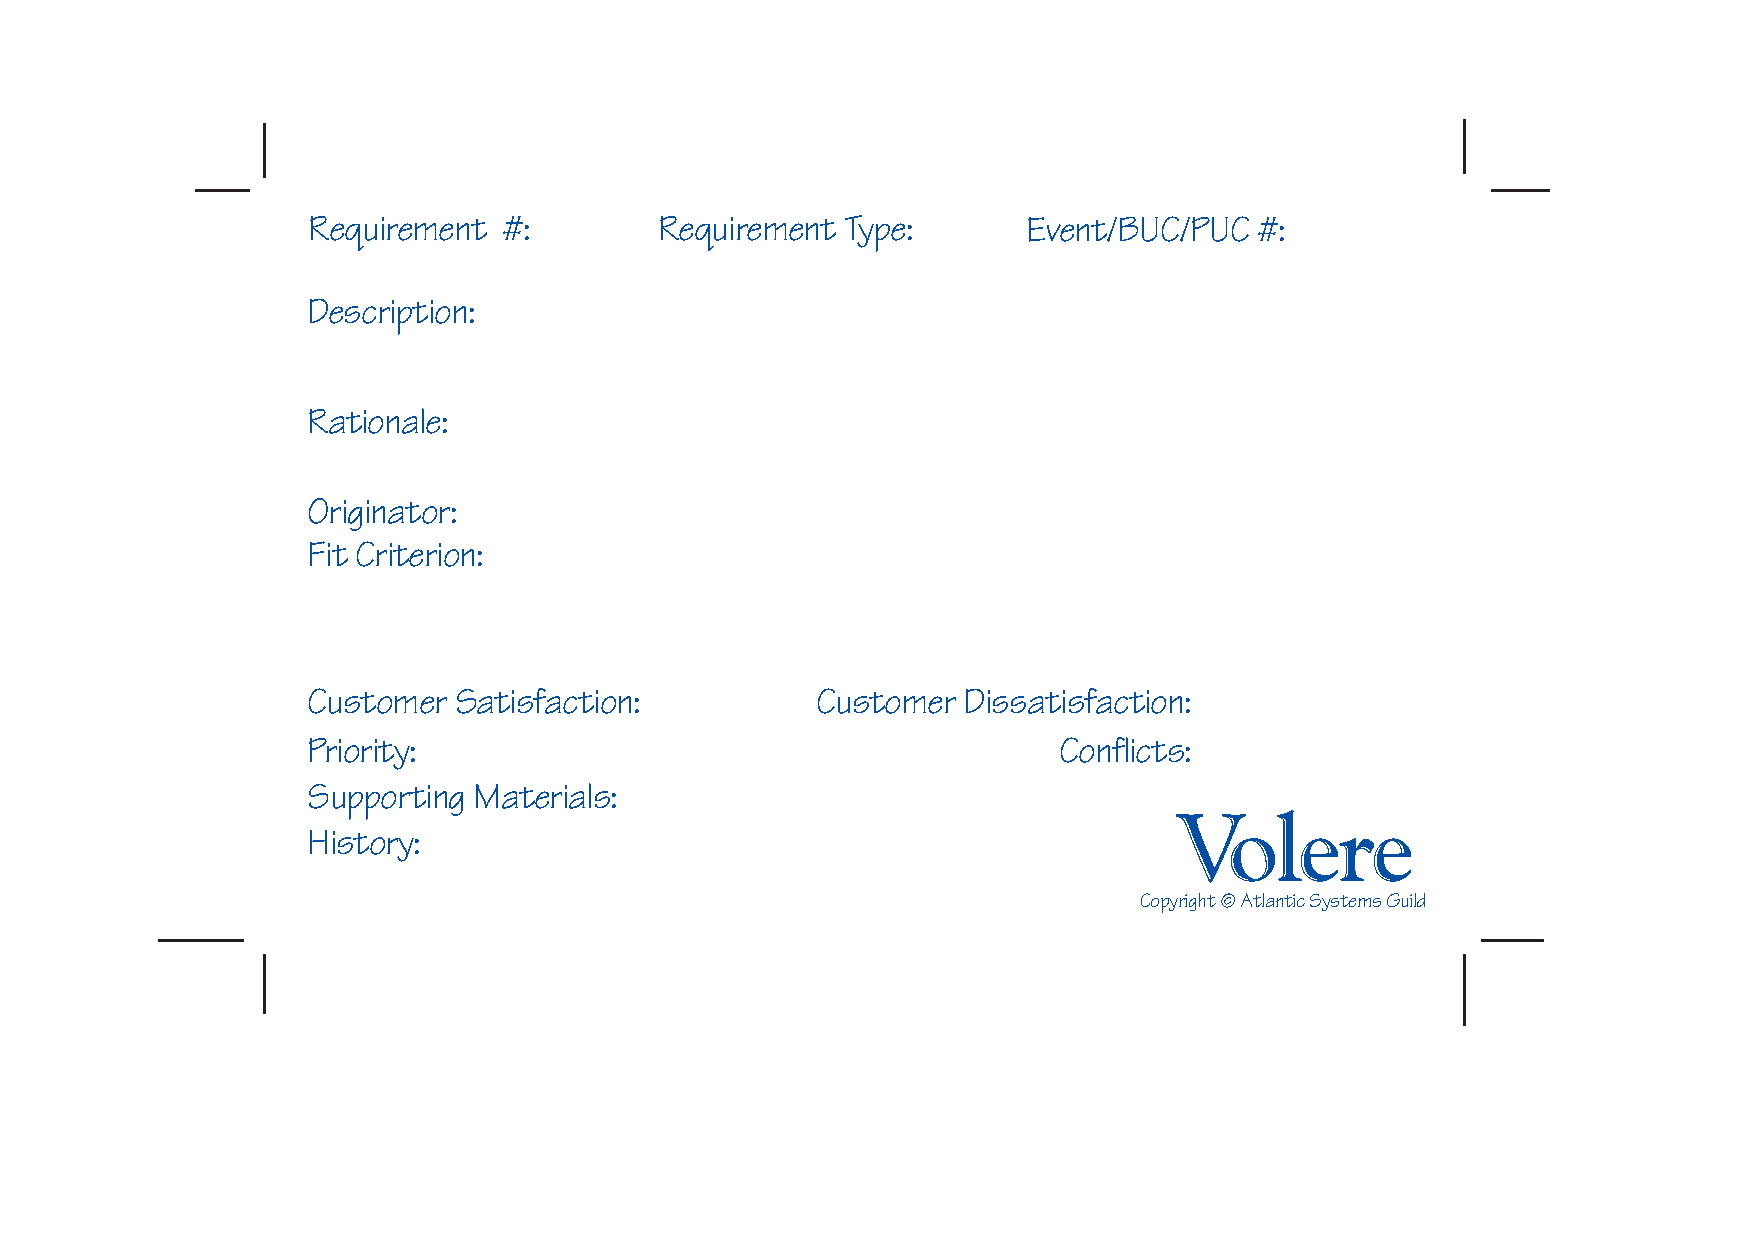
\includegraphics[scale=0.6]{img/snowcard.pdf}
	\caption{Volere Snow Card}
	{\footnotesize Quelle: \cite{VolereSnowCard}}
	\label{abb:volereSnowCard}
	%		{\scriptsize \textit{Alle Rechte, einschließlich der Vervielfältigung, Veröffentlichung, Bearbeitung und Übersetzung bleiben der SV Informatik GmbH vorbehalten.}}
\end{figure}

Die folgende Liste wurde in Anlehnung an die Quelle \cite{VolereRequirmentsSpecTemplate} erstellt.

\begin{minipage}{\linewidth}
	\begin{itemize}\label{abb:volereReqSpec}
		\item Projekt-Treiber
		\begin{enumerate}
			\item Zweck des Projekts
			\item Auftraggeber, Kunde und andere Stakeholder
			\item Nutzer des Produkts
		\end{enumerate}
		\item Projekt-Randbedingungen
		\begin{enumerate}
			\item Einschränkungen
			\item Namenskonventionen und Definitionen
			\item Relevante Fakten und Annahmen
		\end{enumerate}
		\item Funktionale Anforderungen
		\begin{enumerate}
			\item Arbeitsrahmen
			\item Systemgrenzen
			\item Funktionale und Daten-Anforderungen
		\end{enumerate}
		\item Nicht-funktionale Anforderungen
		\begin{enumerate}
			\item Look-and-Feel-Anforderungen
			\item Usability-Anforderungen
			\item Performanz-Anforderungen
			\item Operationale und Umfeld-Anforderungen
			\item Wartungs- und Unterstützungsanforderungen
			\item Sicherheitsanforderungen
			\item Kulturelle und politische Anforderungen
			\item Rechtliche Anforderungen
		\end{enumerate}
		\item Projekt-Aspekte
		\begin{enumerate}
			\item Offene Punkte
			\item Standardlösungen
			\item Neu aufgetretene Probleme
			\item Installationsaufgaben
			\item Migrationstätigkeiten
			\item Risiken
			\item Kosten
			\item Nutzerdokumentation
			\item Zurückgestellte Anforderungen
			\item Lösungsideen
		\end{enumerate}
	\end{itemize}
\end{minipage}

\clearpage
\begin{figure}[H]
	\centering
	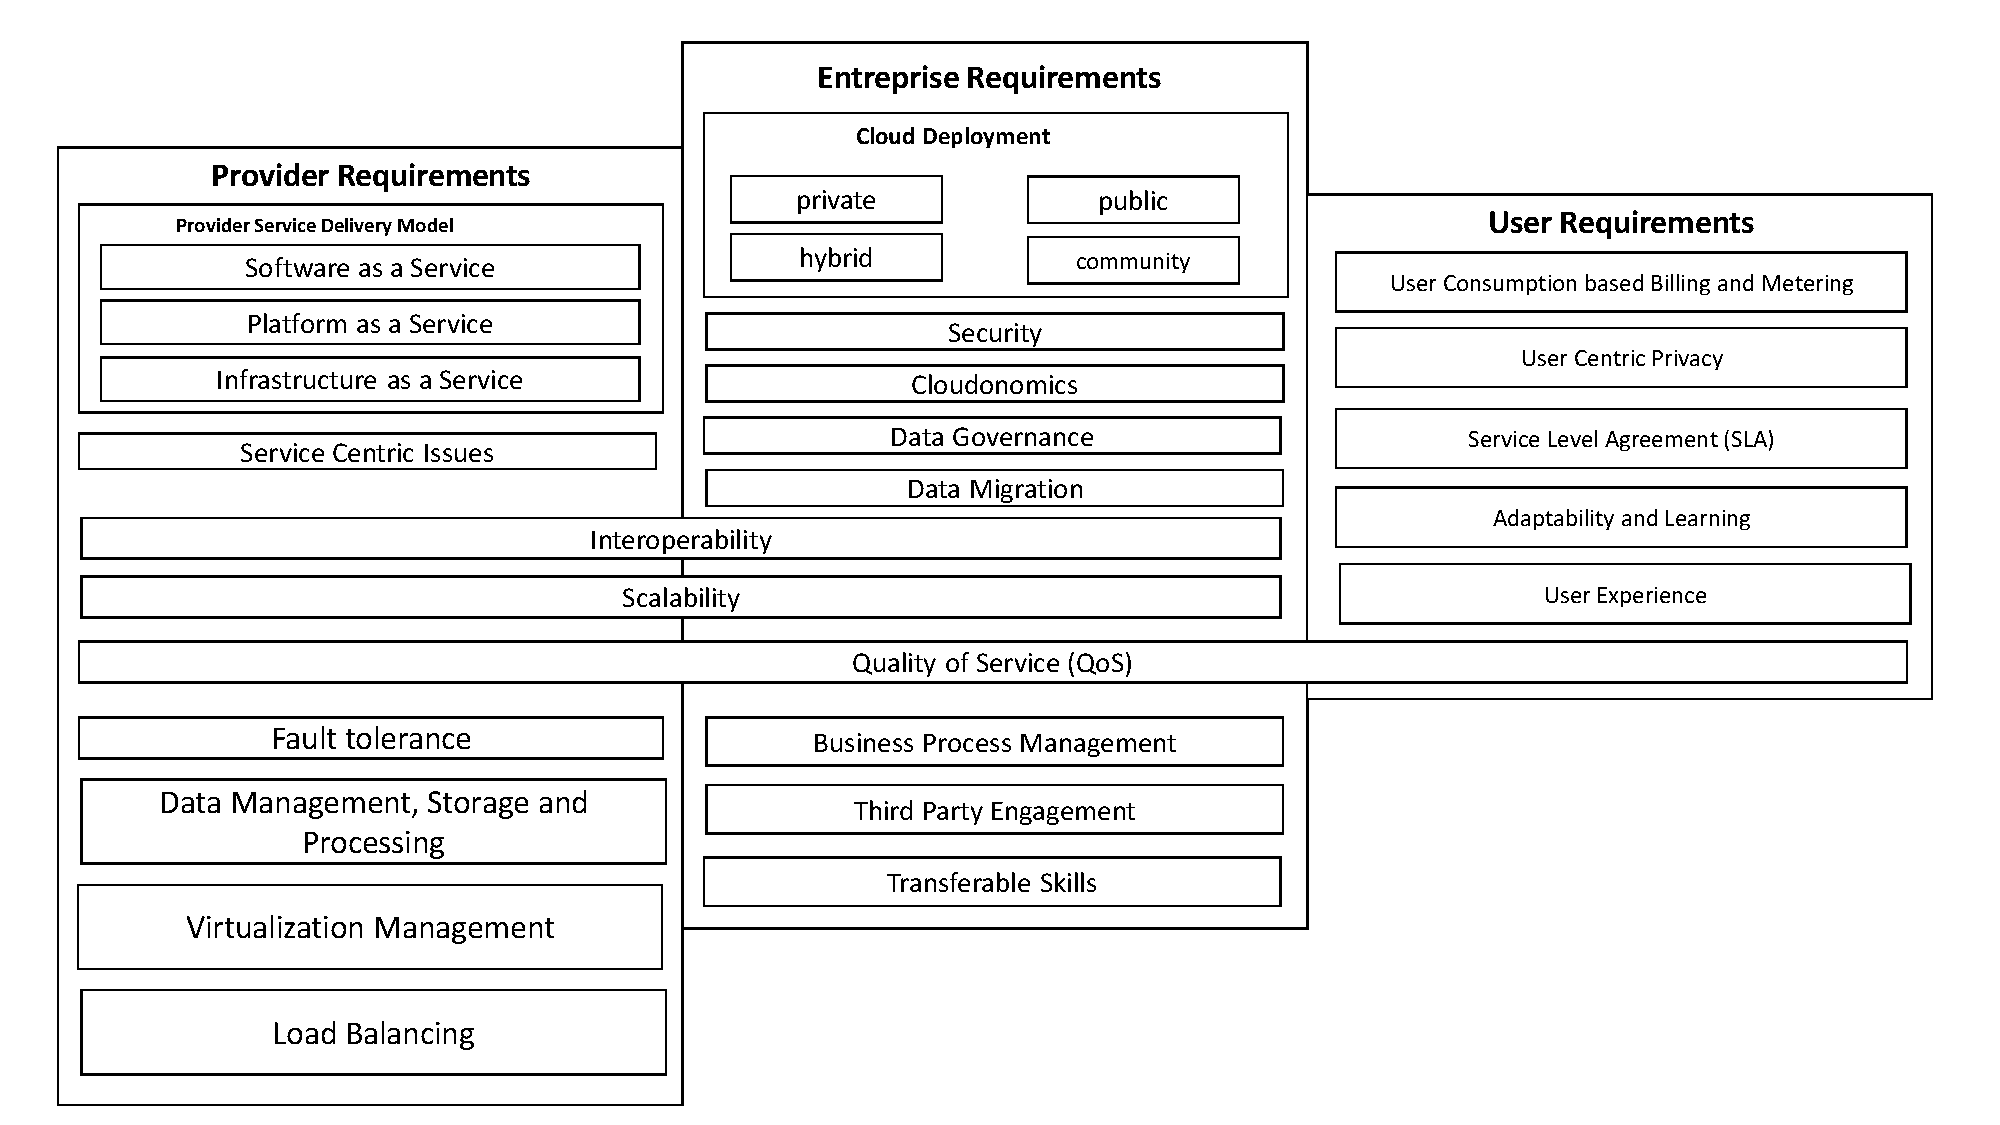
\includegraphics[scale=0.50, angle=90]{img/cloudreq.pdf}
	\caption{Ebenen der \enquote{Cloud}-Anforderungsanalyse}
	{\footnotesize Quelle: in Anlehnung an \cite{rimal_architectural_2011}}
	\label{abb:cloudreq}
	%		{\scriptsize \textit{Alle Rechte, einschließlich der Vervielfältigung, Veröffentlichung, Bearbeitung und Übersetzung bleiben der SV Informatik GmbH vorbehalten.}}
\end{figure}

\clearpage
\section{Statistiken zum Themengebiet \ac{Cloud-C}}

\begin{figure}[H]
	\centering
	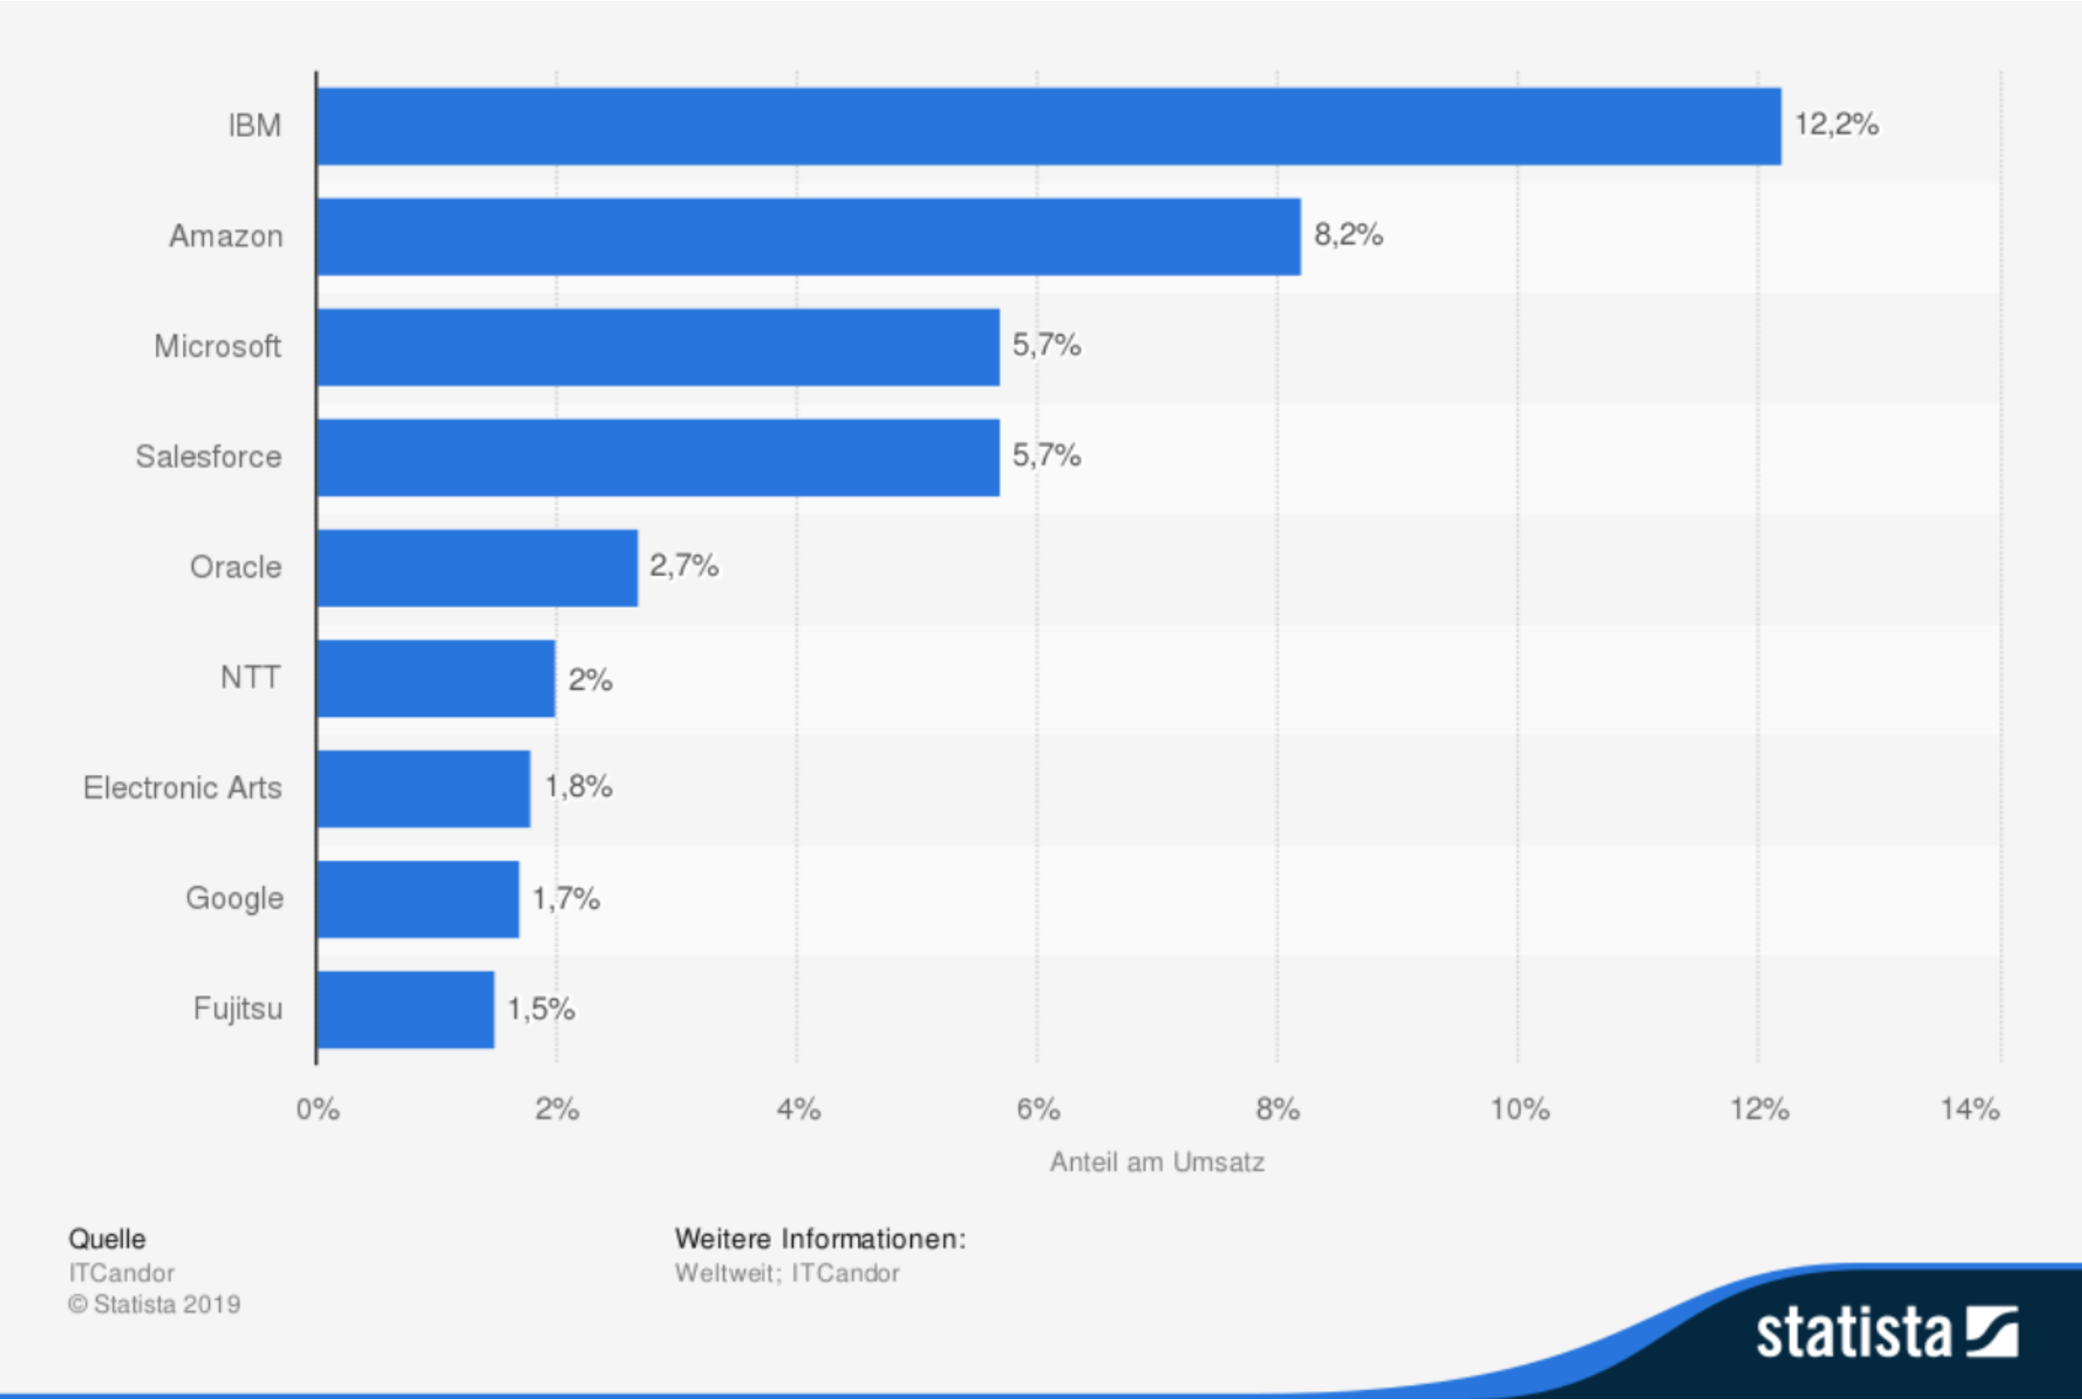
\includegraphics[scale=0.43]{img/statistic_id150979_marktanteile-der-fuehrenden-unternehmen-im-bereich-cloud-computing-weltweit-2019.pdf}
	\caption{Marktanteile der führenden Unternehmen am Umsatz im Bereich Cloud Computing weltweit von Juli 2018 bis Juni 2019}
	{\footnotesize Quelle: \cite{itcandor_cloud_2019}}
	\label{abb:marktanteileCC19}
	%		{\scriptsize \textit{Alle Rechte, einschließlich der Vervielfältigung, Veröffentlichung, Bearbeitung und Übersetzung bleiben der SV Informatik GmbH vorbehalten.}}
\end{figure}

\begin{figure}[H]
	\centering
	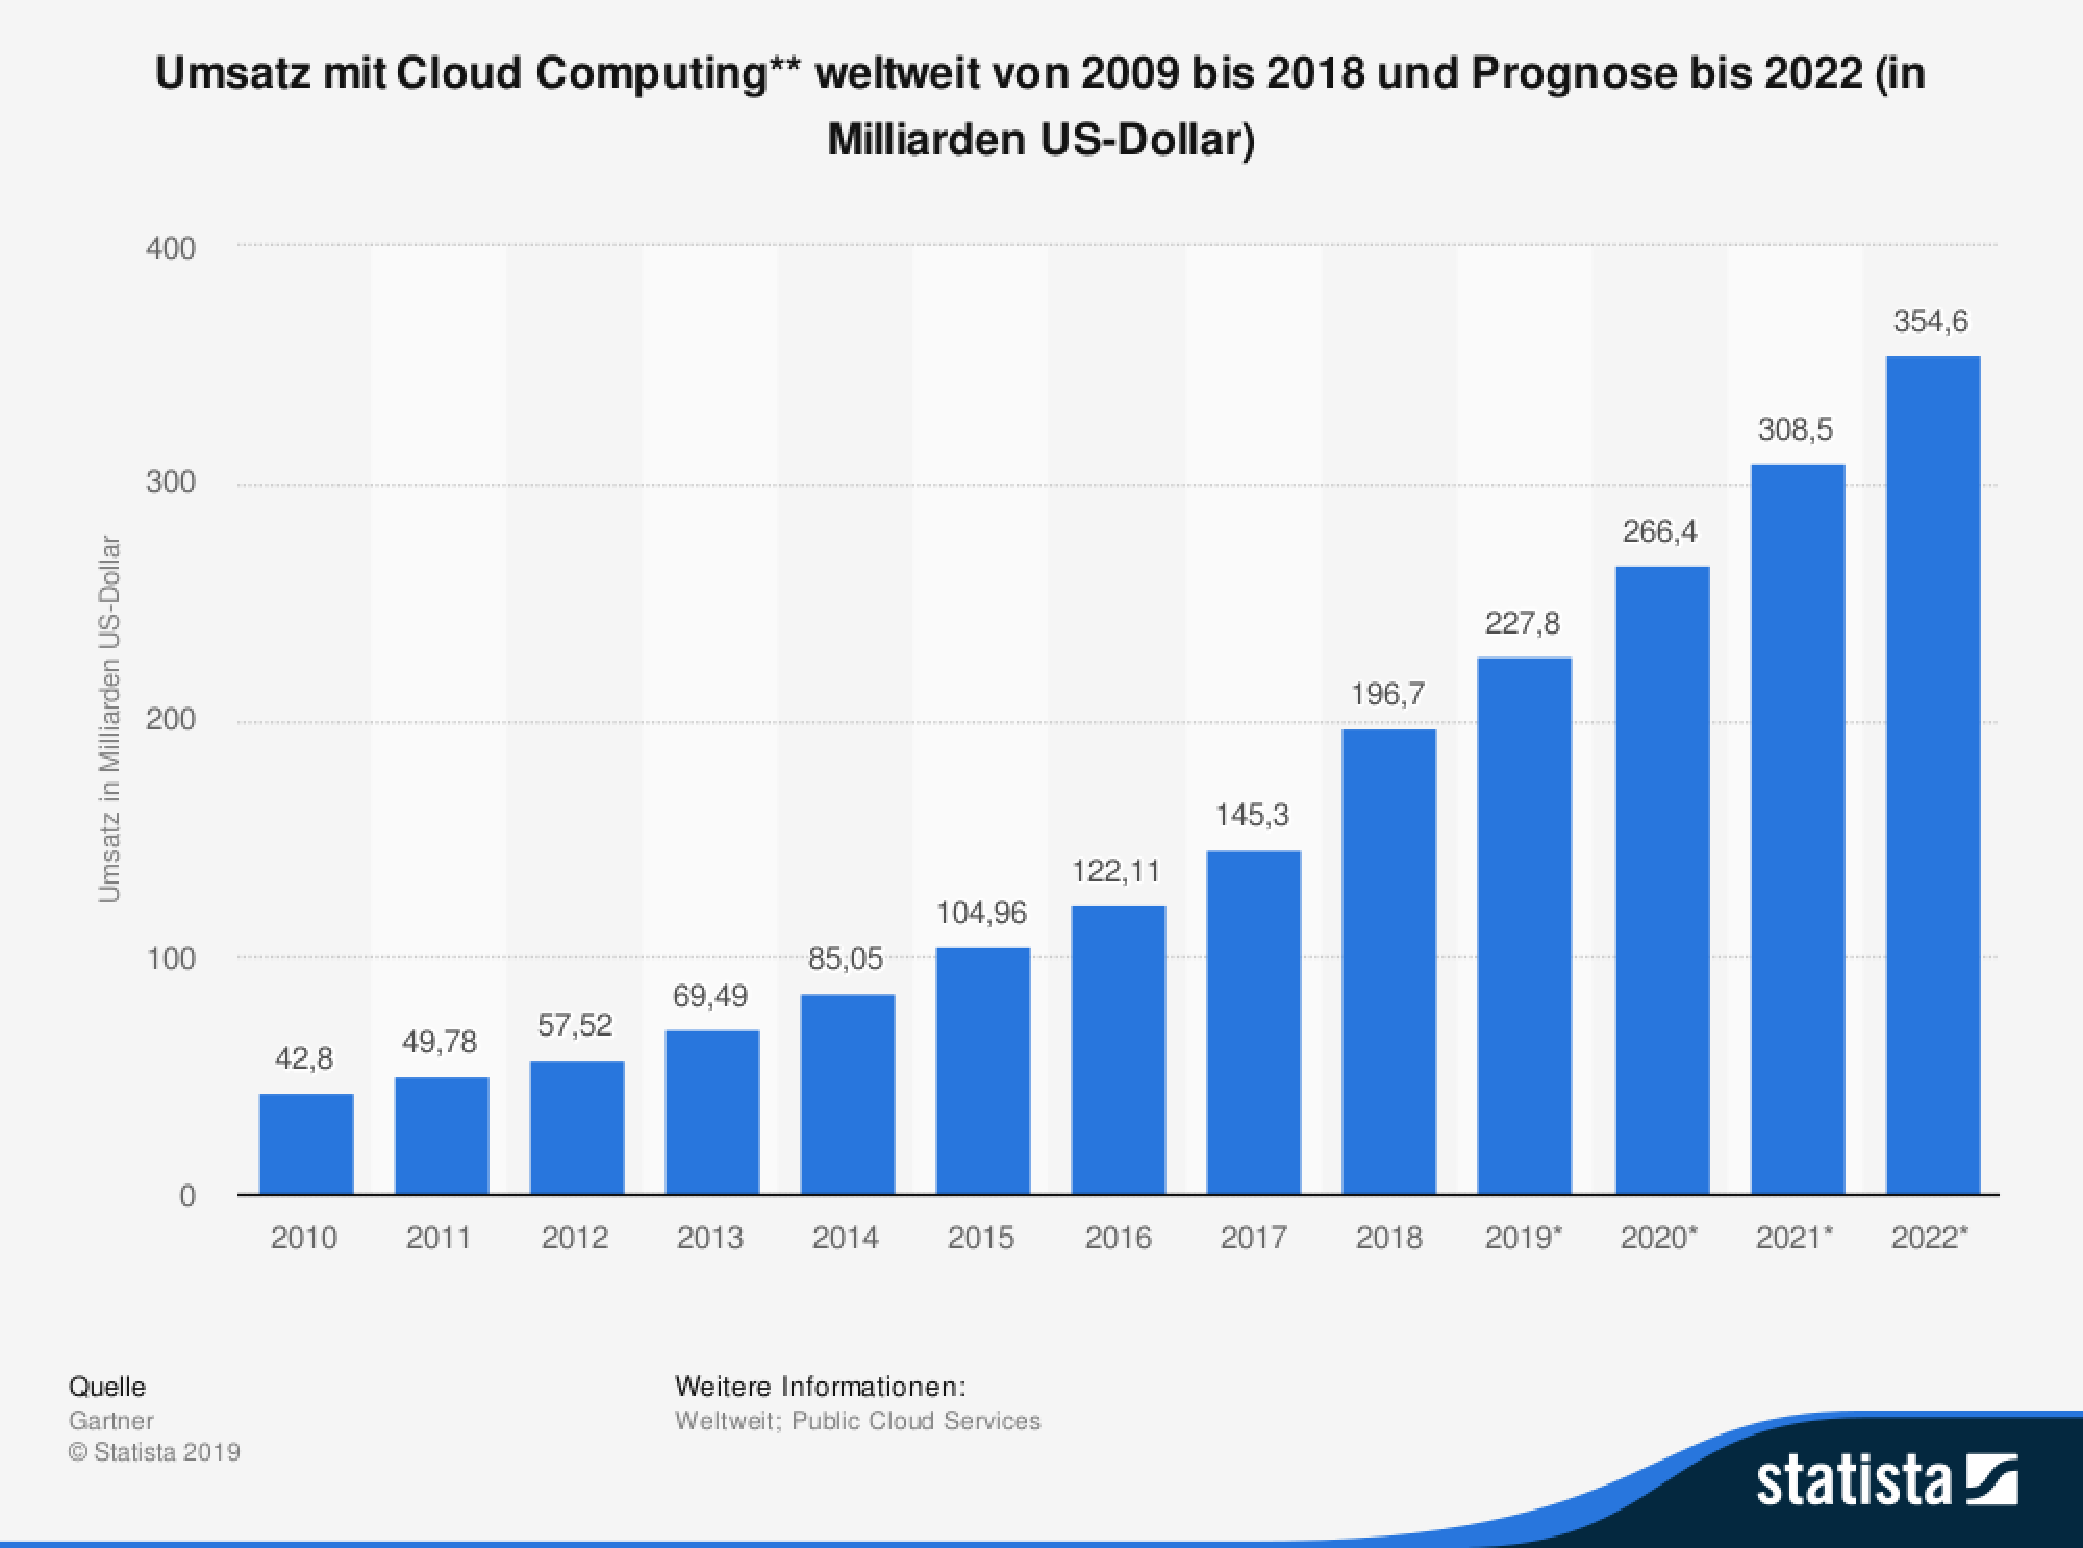
\includegraphics[scale=0.43]{img/statistic_id195760_prognose-zum-umsatz-mit-cloud-computing-weltweit-bis-2022.pdf}
	\caption{Umsatz mit Cloud-Computing weltweit von 2009 bis 2018 und Prognose bis 2022 }
	{\footnotesize Quelle: \cite{gartner_cloud_2019}}
	\label{abb:umsatzprognoseCC}
	%		{\scriptsize \textit{Alle Rechte, einschließlich der Vervielfältigung, Veröffentlichung, Bearbeitung und Übersetzung bleiben der SV Informatik GmbH vorbehalten.}}
\end{figure}

\section{Ergänzungen zum Kapitel Container(-isierung) und Orchestrierung}

\begin{figure}[H]
	\centering
	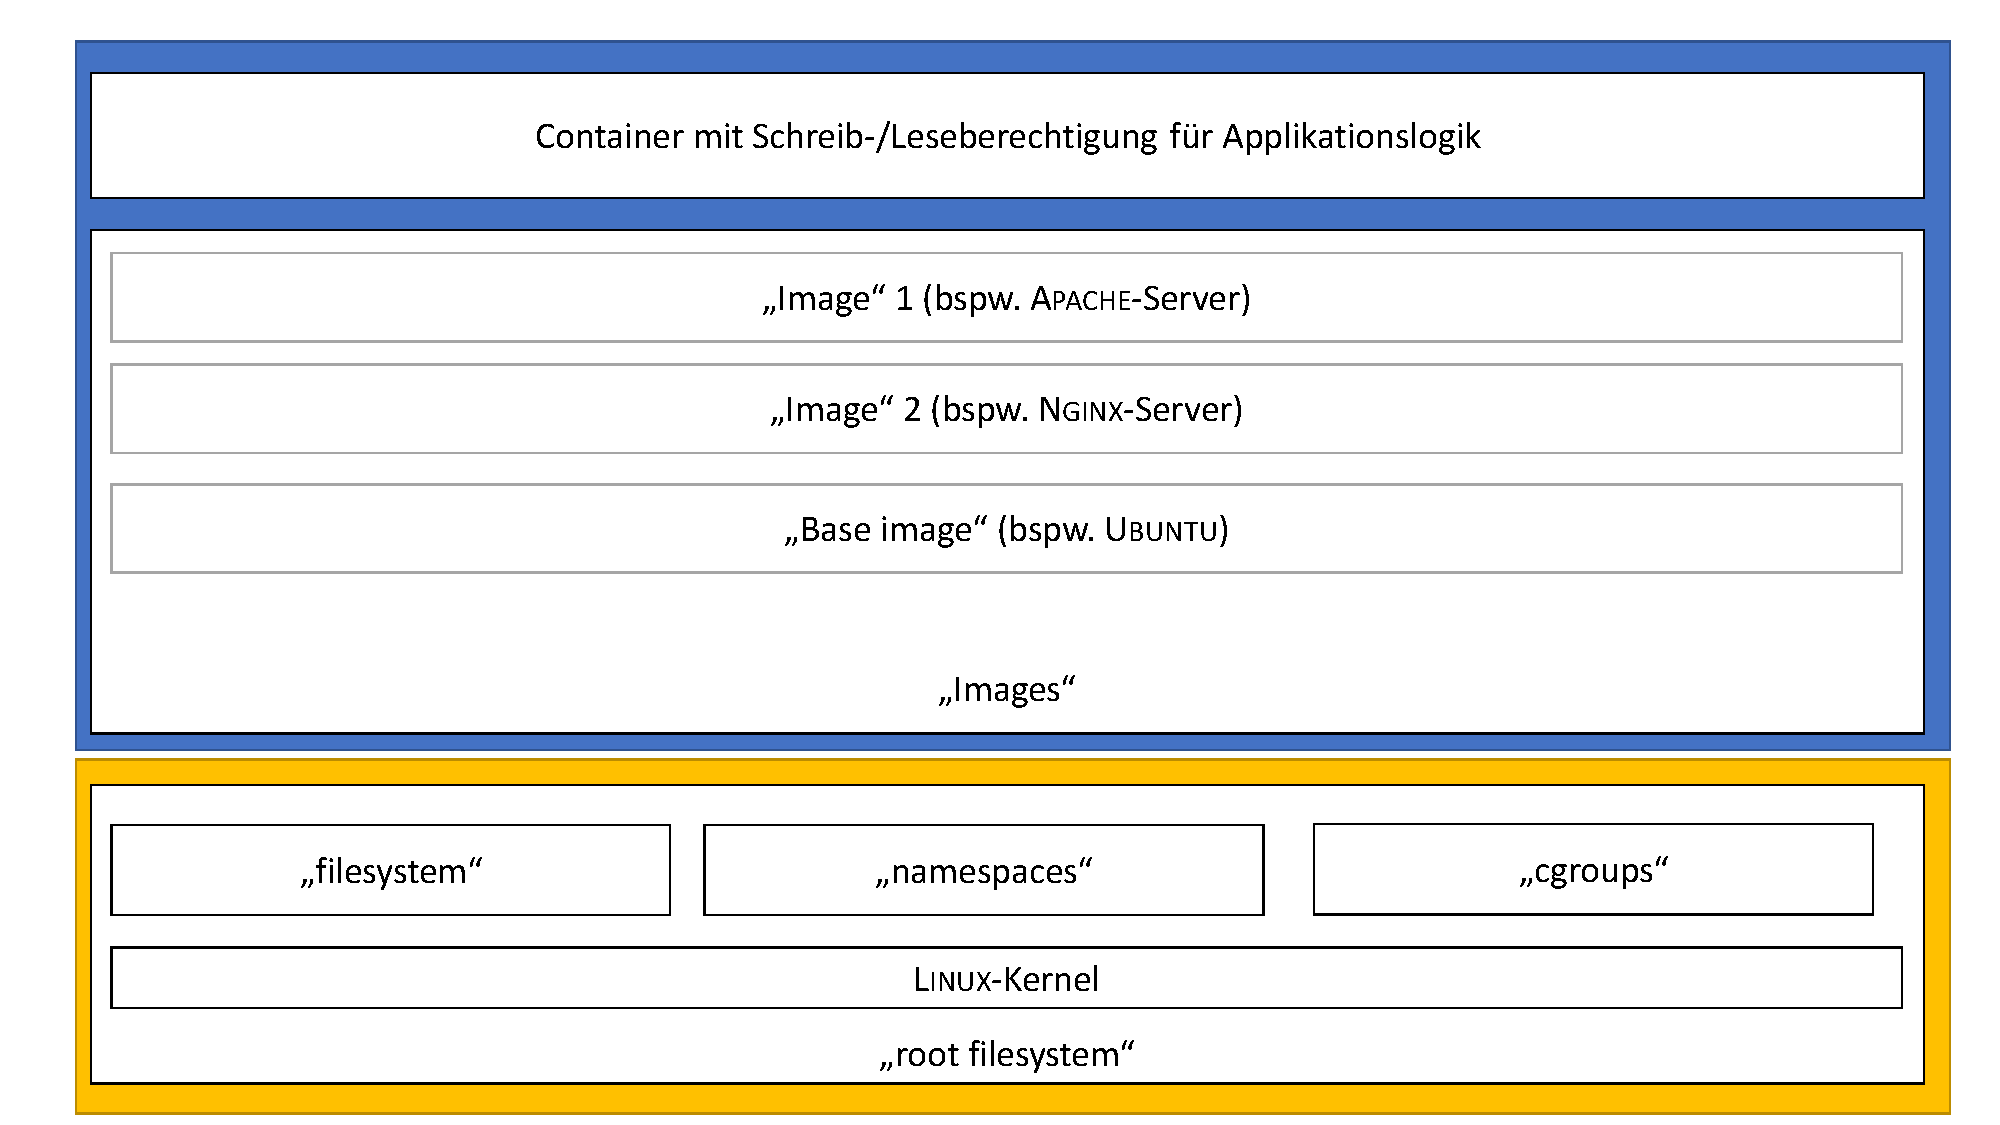
\includegraphics[scale=0.45]{img/containerImageArch.pdf}
	\caption{Architektur des Container-\enquote{Images}}
	{\footnotesize Quelle: in Anlehnung an \cite{pahl_containerization_2015}}
	\label{abb:containerArch}
	%		{\scriptsize \textit{Alle Rechte, einschließlich der Vervielfältigung, Veröffentlichung, Bearbeitung und Übersetzung bleiben der SV Informatik GmbH vorbehalten.}}
\end{figure}

Hierbei ist zu beachten, dass das orange gefärbte die Funktionalitäten der \textsc{Docker}-\enquote{Engine} und das blau gefärbte die möglichen Bestandteile eines \textsc{Docker}-\enquote{Images} darstellen soll.


\begin{figure}[H]
	\centering
	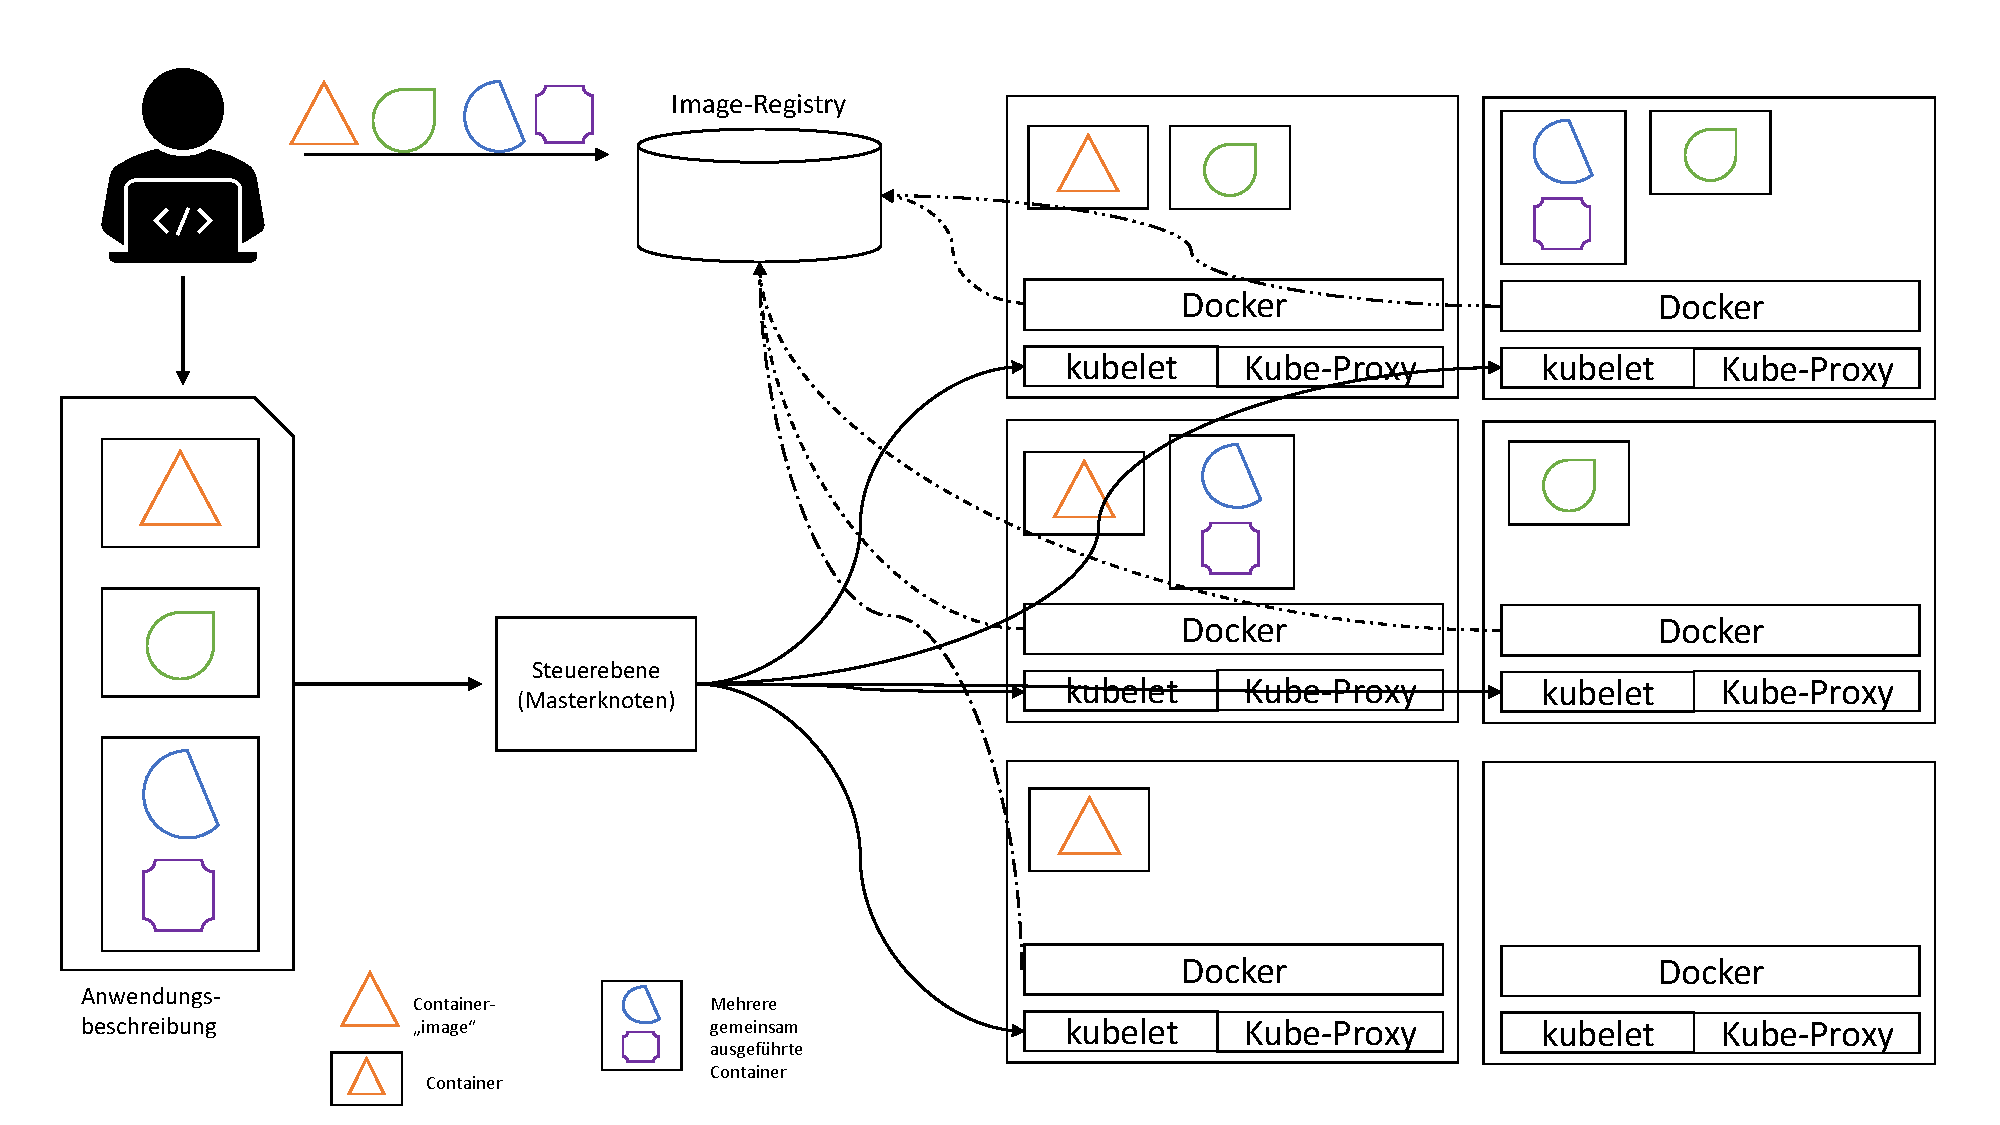
\includegraphics[scale=0.46]{img/k8sArch.pdf}
	\caption{Überblick über eine \textsc{Kubernetes}-Architektur}
	{\footnotesize Quelle: in Anlehnung an \cite[][S.23]{luksa_kubernetes_2018}}
	\label{abb:k8sArch}
	%		{\scriptsize \textit{Alle Rechte, einschließlich der Vervielfältigung, Veröffentlichung, Bearbeitung und Übersetzung bleiben der SV Informatik GmbH vorbehalten.}}
\end{figure}

\begin{figure}[H]
	\centering
	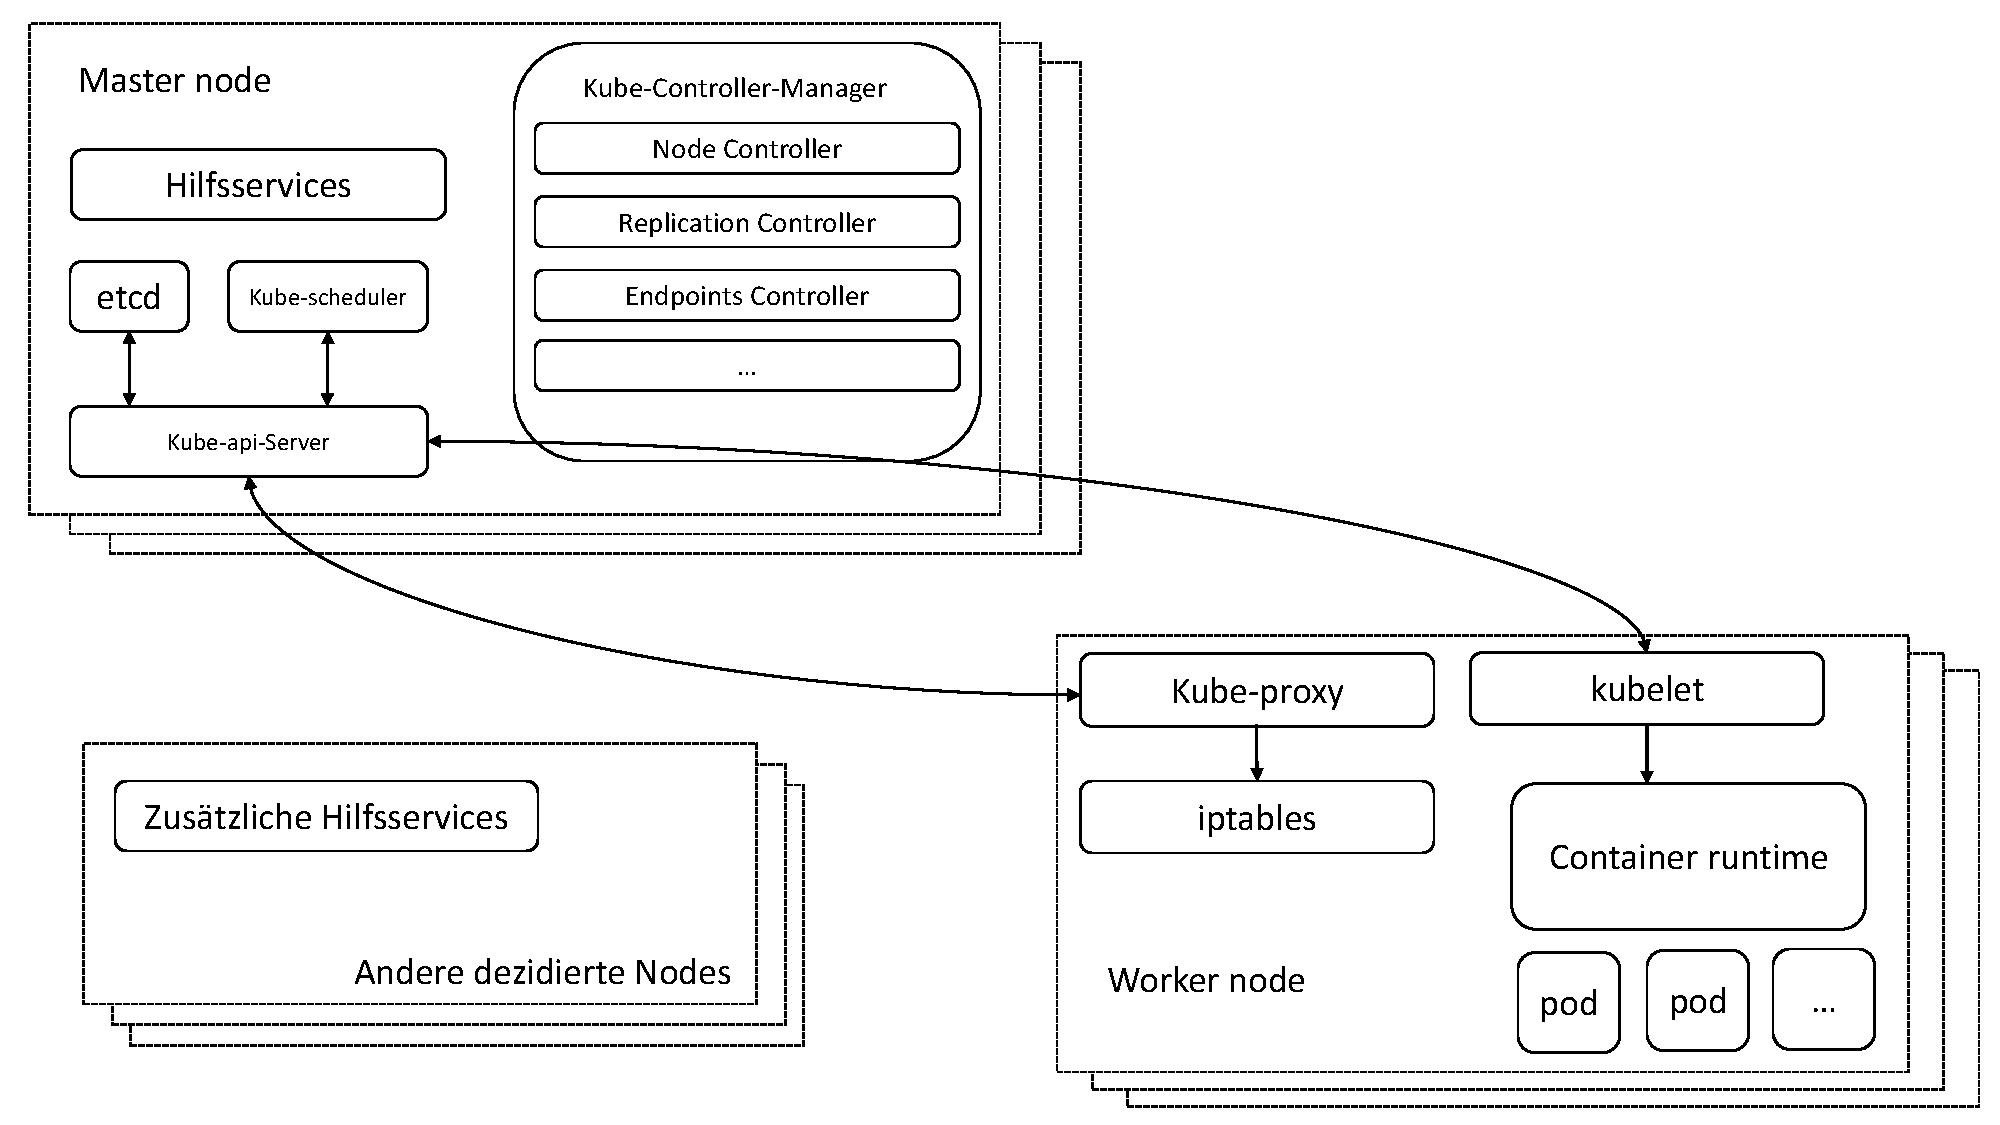
\includegraphics[scale=0.46]{img/k8sArchInteraktion.pdf}
	\caption{Architektur der \enquote{\ac{K8s}}-Interaktion}
	{\footnotesize Quelle: in Anlehnung an \cite[][S.15]{caban_architecting_2019}}
	\label{abb:k8sArchInteraktion}
	%		{\scriptsize \textit{Alle Rechte, einschließlich der Vervielfältigung, Veröffentlichung, Bearbeitung und Übersetzung bleiben der SV Informatik GmbH vorbehalten.}}
\end{figure}

\chapter{Ergänzungen zur Forschungsfrage zwei} \label{appendixFF2}
In diesem Teil des Anhangs sind Ergänzungen zur Forschungsfrage zwei des Kapitels \vref{ff2} beschrieben.

\section{Entscheidung über die Notwendigkeit eines \enquote{Business Case}}

\begin{figure}[H]
	\centering
	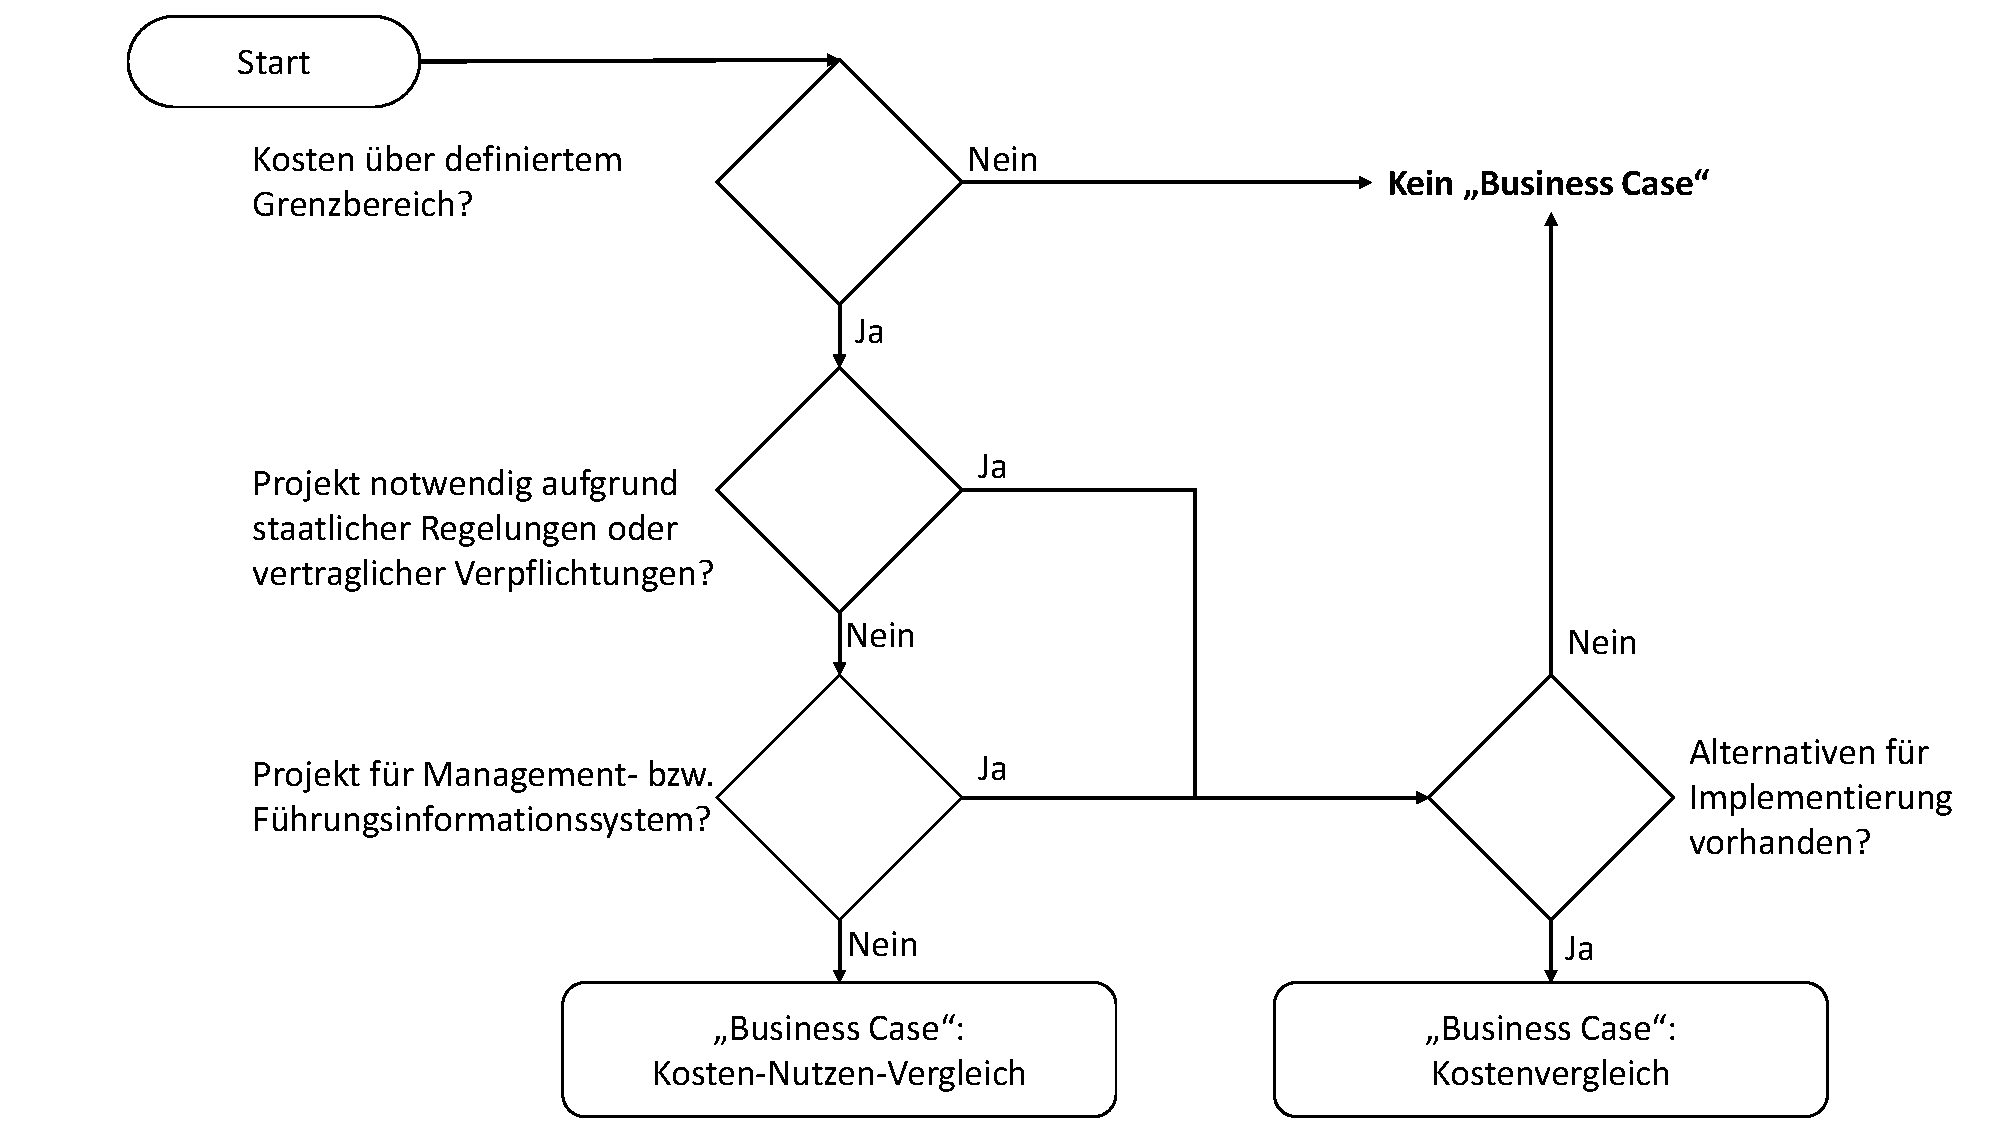
\includegraphics[scale=0.48]{img/entscheidungBC.pdf}
	\caption{Notwendigkeit eines \enquote{Business Case}}
	{\footnotesize Quelle: in Anlehnung an \cite[][S.29]{brugger_it_2009}}
	\label{abb:entscheidungBC}
	%		{\scriptsize \textit{Alle Rechte, einschließlich der Vervielfältigung, Veröffentlichung, Bearbeitung und Übersetzung bleiben der SV Informatik GmbH vorbehalten.}}
\end{figure}

\section{Vor-/Nachteile der internen beziehungsweise externen Erstellung eines \enquote{Business Case}}\label{appendixVorNachteileErstellungBC}

\begin{table*}[h!]
	\centering
	\ra{1.3} %more space beetween rules
	
	\begin{tabular}{@{}ll@{}}\toprule[1.5pt]
		
		\textbf{Vorteile} & \textbf{Nachteile} \\ \midrule
		
		% below rules with content
		Neutralität & Kein Wissenstransfer \\
		Verfügbarkeit & Kosten, egal ob der \enquote{Business Case} rentabel ist\\
		Effiziente Erstellung & hohe Kosten im Vergleich zur internen Erstellung \\
		Glaubwürdigkeit & Abhängigkeit \\
		Qualität & Verlust der firmeninternen Standards \\
		Innovation & \\
		Schlichtung & \\
		
		\bottomrule[1.5pt]
	\end{tabular}
	
	\caption{Überblick über die Vor-/Nachteile der externen Erstellung eines \enquote{Business Case}}
	{\footnotesize Quelle: in Anlehnung an \cite[][S.34]{brugger_it_2009}}
	\label{tab:externVorNachteile}
	
\end{table*}

\begin{table*}[h!]
	\centering
	\ra{1.3} %more space beetween rules
	
	\begin{tabular}{@{}ll@{}}\toprule[1.5pt]
		
		\textbf{Vorteile} & \textbf{Nachteile} \\ \midrule
		
		% below rules with content
		Wissensaufbau & Verfügbarkeit \\
		Qualität & Effizienzverlust bei rein technischen/operativen Mitarbeitern \\
		\enquote{Teamwork} & Glaubwürdigkeit \\
		Standardisierung & Qualitätskontrolle durch \enquote{Controlling}-Division \\
		
		\bottomrule[1.5pt]
	\end{tabular}
	
	\caption{Überblick über die Vor-/Nachteile der internen Erstellung eines \enquote{Business Case}}
	{\footnotesize Quelle: in Anlehnung an \cite[][S.34]{brugger_it_2009}}
	\label{tab:internVorNachteile}
	
\end{table*}

\begin{figure}[H]
	\centering
	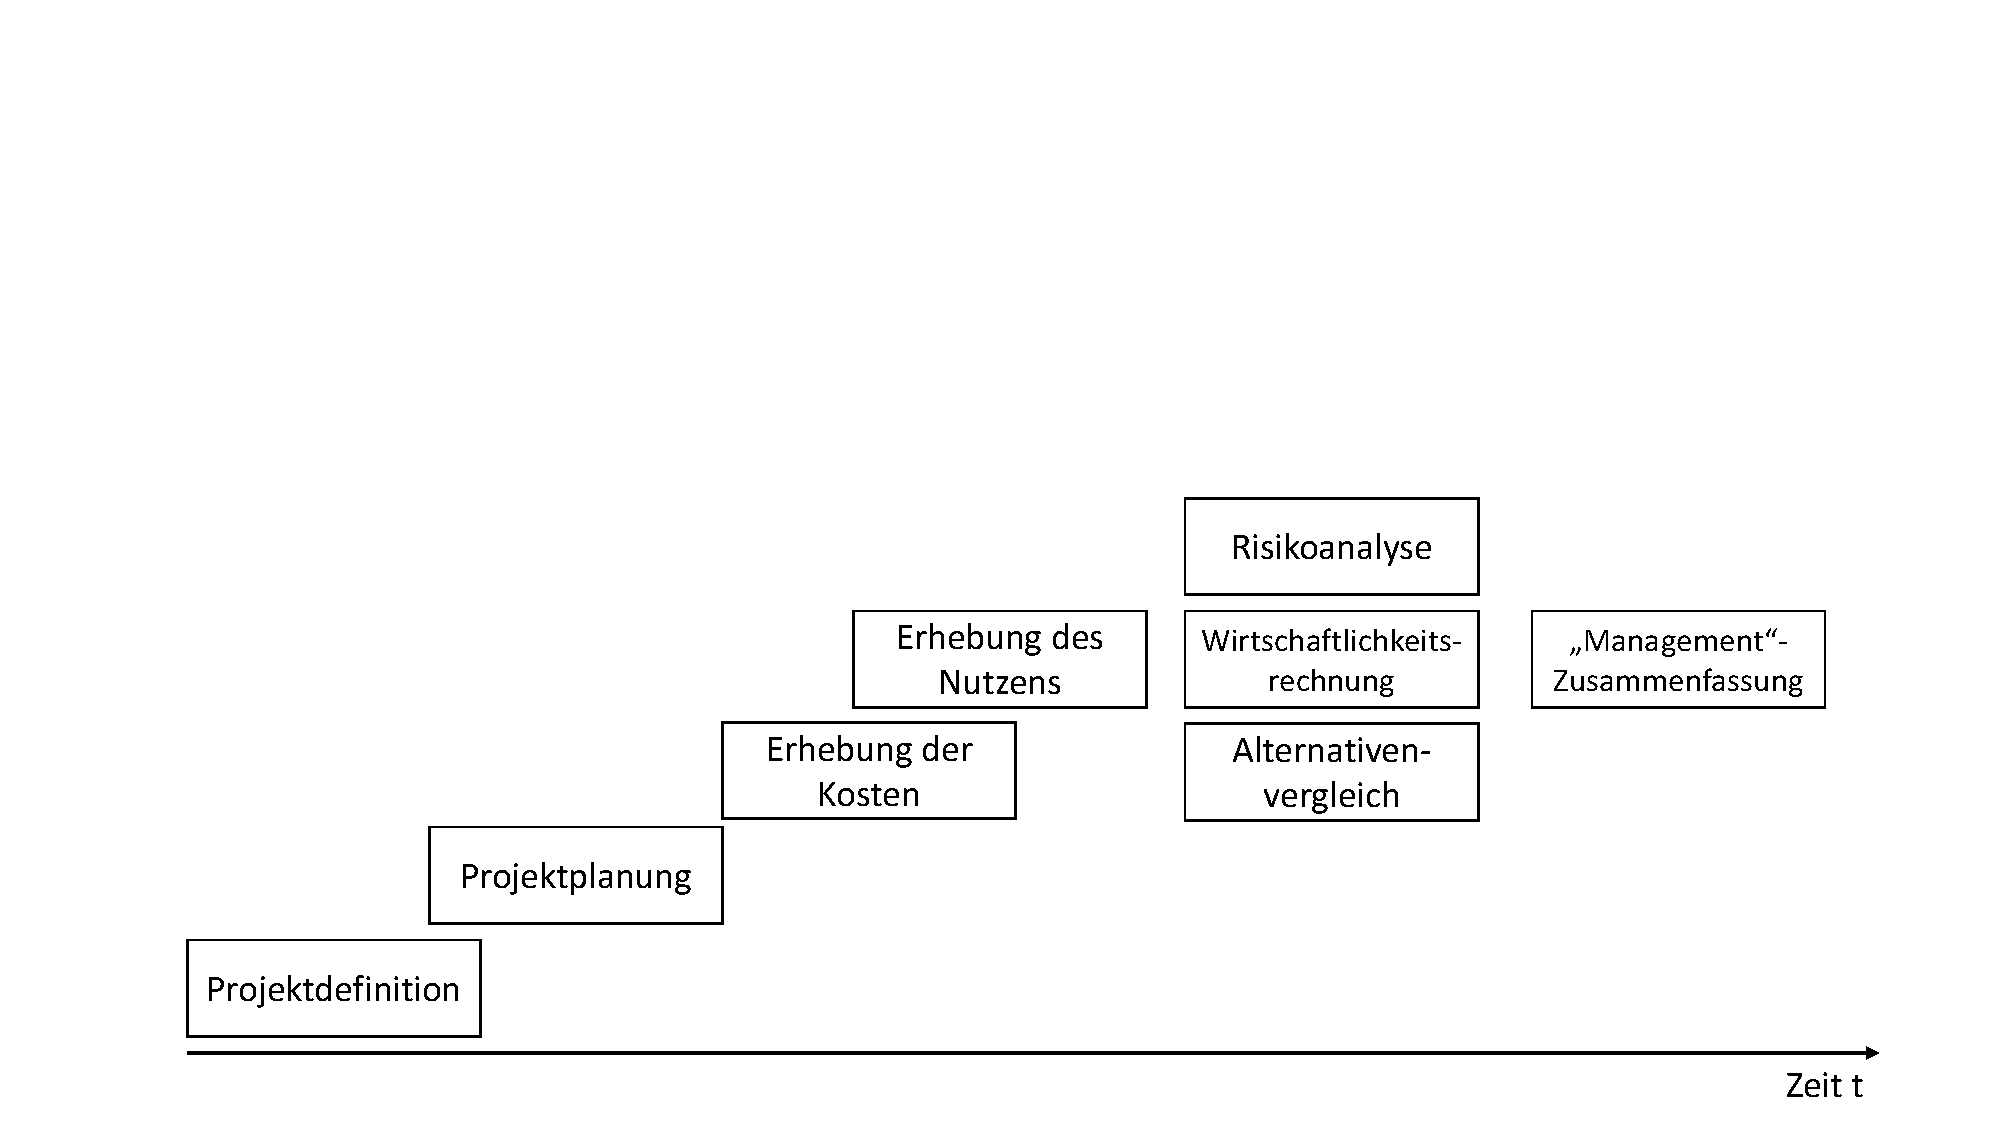
\includegraphics[scale=0.48]{img/chronoBC.pdf}
	\caption{Chronologische Abfolge der Entwicklungsphase eines \enquote{Business Case}}
	{\footnotesize Quelle: in Anlehnung an \cite[][]{herman_is_2009}}
	\label{abb:entwicklungBC}
	%		{\scriptsize \textit{Alle Rechte, einschließlich der Vervielfältigung, Veröffentlichung, Bearbeitung und Übersetzung bleiben der SV Informatik GmbH vorbehalten.}}
\end{figure}

\chapter{Ergänzungen zur Forschungsfrage drei} \label{appendixFF3}
In diesem Teil des Anhangs sind Ergänzungen zur Forschungsfrage drei des Kapitels \vref{ff3} beschrieben.

\section{\enquote{Plan-Do-Check-Act}-Regelkreis}

\begin{figure}[H]
	\centering
	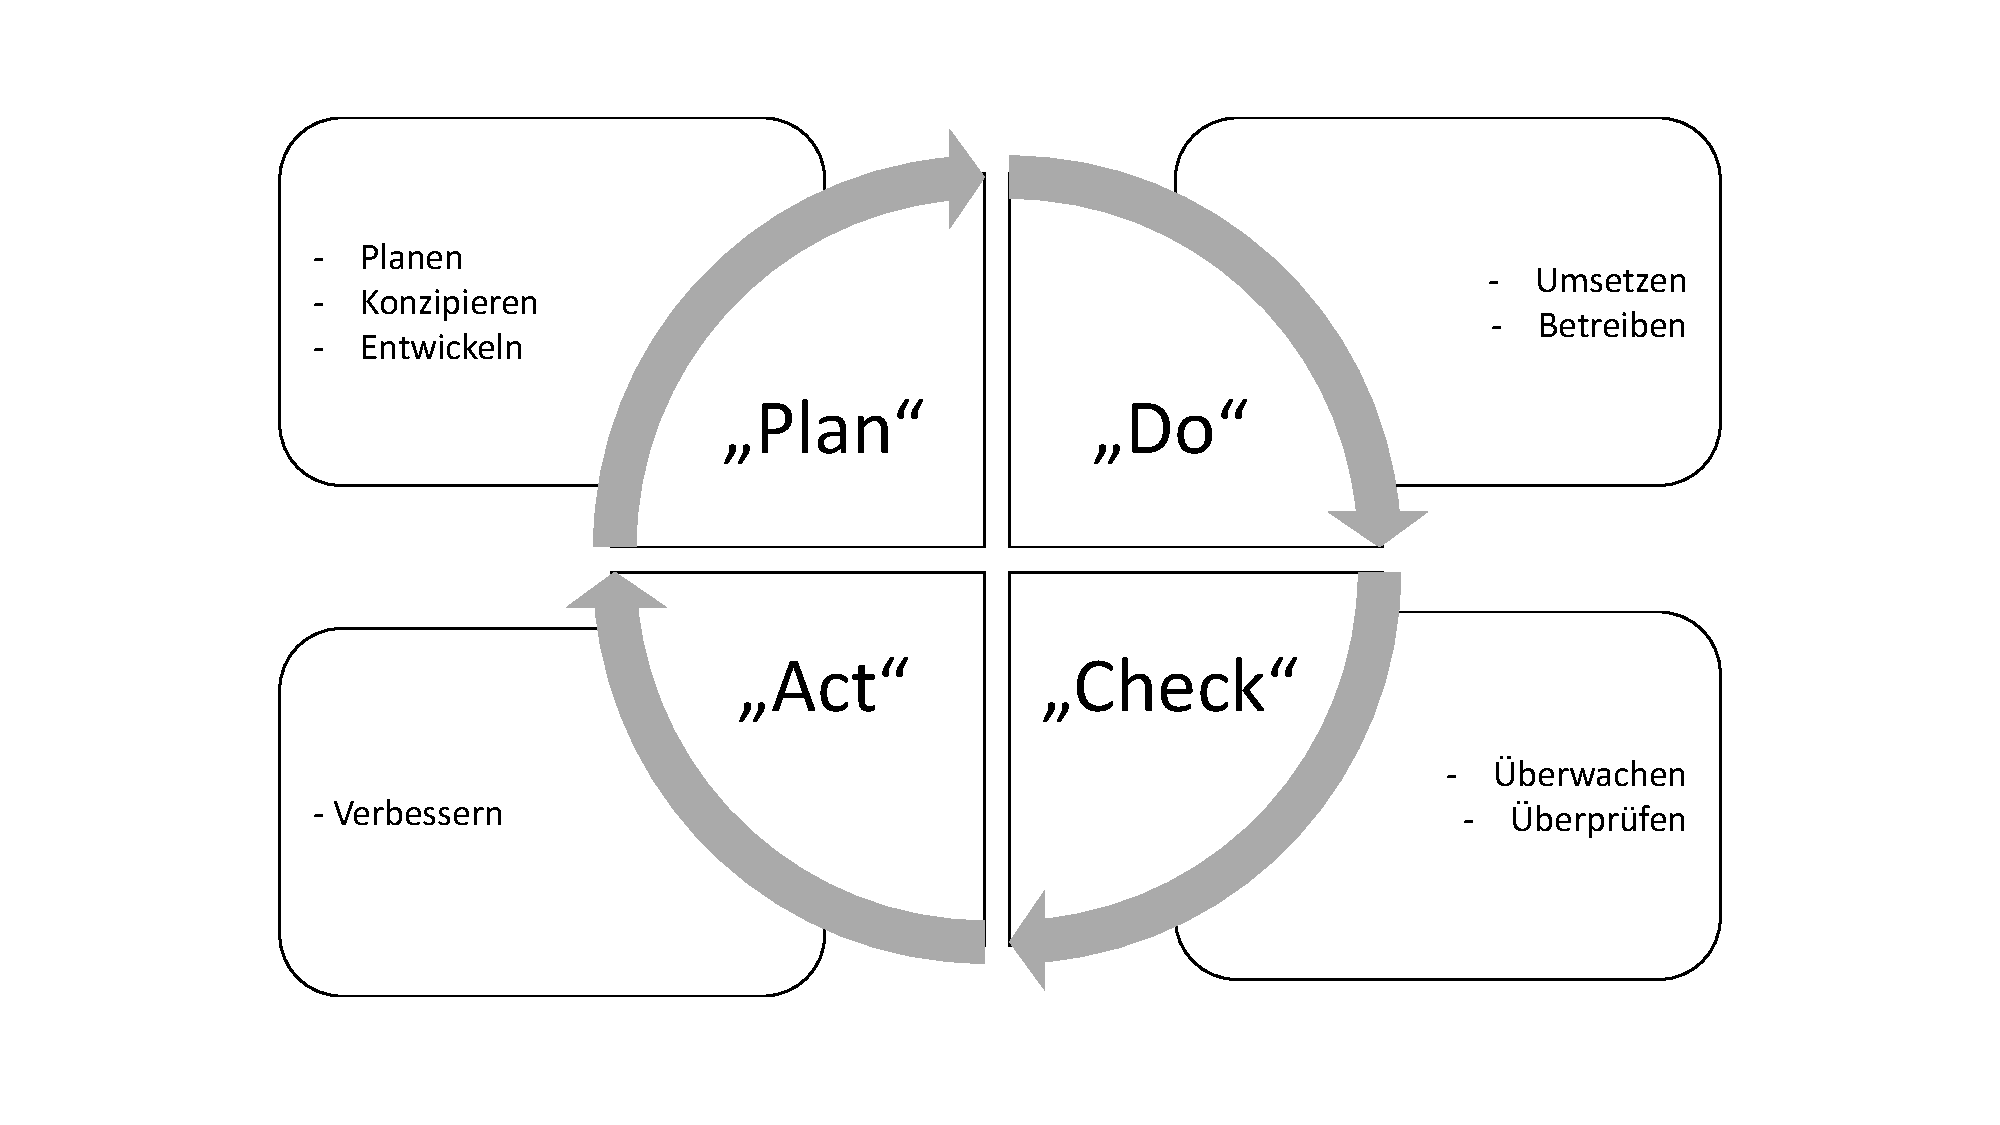
\includegraphics[scale=0.51]{img/planDoCheckAct.pdf}
	\caption{Der \enquote{Plan-Do-Check-Act}-Regelkreis}
	{\footnotesize Quelle: in Anlehnung an \cite[][S.12]{kersten_it-sicherheitsmanagement_2020}}
	\label{abb:planDoCheckAct}
	%		{\scriptsize \textit{Alle Rechte, einschließlich der Vervielfältigung, Veröffentlichung, Bearbeitung und Übersetzung bleiben der SV Informatik GmbH vorbehalten.}}
\end{figure}

\clearpage % neue Seite
\section{Checkliste zur Vorbereitung der \ac{ISMS}-Einführung}
\begin{table*}[h!]
	\centering
	\ra{1.3} %more space beetween rules
	
	\begin{tabular}{@{}lp{10cm}l@{}}\toprule[1.5pt]
		
		\textbf{Aktion} & \textbf{Gegenstand} & \textbf{Erfüllt?} \\ \midrule
		% below rules with content
		
		1 & Sind die Normen (27000, 27001, 27002) in aktueller elektronischer
		Form vorhanden? & $\square$ \\
		2 & Sind die Vorteile und der Nutzen eines ISMS erläutert worden? & $\square$ \\
		3 & Ist ein Grob-Abgleich mit ISO 27001 erfolgt? (Ziel: erste
		Aufwandsabschätzung) & $\square$ \\
		4 & Ist eine Entscheidung zur Orientierung an der ISO 27001
		getroffen worden? & $\square$ \\
		5 & Denken wir in Management-Systemen? Existieren schon andere
		Management-Systeme? & $\square$ \\
		6 & Ist der Begriff ISMS eingeführt? & $\square$ \\
		7 & Denken wir in Geschäftsprozessen und informationstechnischen Anwendungen? & $\square$ \\
		8 & Ist der Anwendungsbereich des ISMS (Scope) zumindest grob
		skizziert? & $\square$ \\
		9 & Sind zumindest die Top Level Assets und deren Asset/Risk
		Owner erfasst worden? & $\square$ \\
		10 & Wurden – zumindest grob – Sicherheitsziele für diese Assets
		festgelegt? & $\square$ \\
				
		\bottomrule[1.5pt]
	\end{tabular}
	
	\caption{Checkliste zur Vorbereitung der \ac{ISMS}-Einführung}
	{\footnotesize{Quelle: in Anlehnung an \cite[][S.15]{kersten_it-sicherheitsmanagement_2020}}}
	\label{tab:checklisteVorbereitungISMS}
	
\end{table*}

\clearpage
\section{Schichtenmodell des IT-Grundschutzes}
\begin{figure}[H]
	\centering
	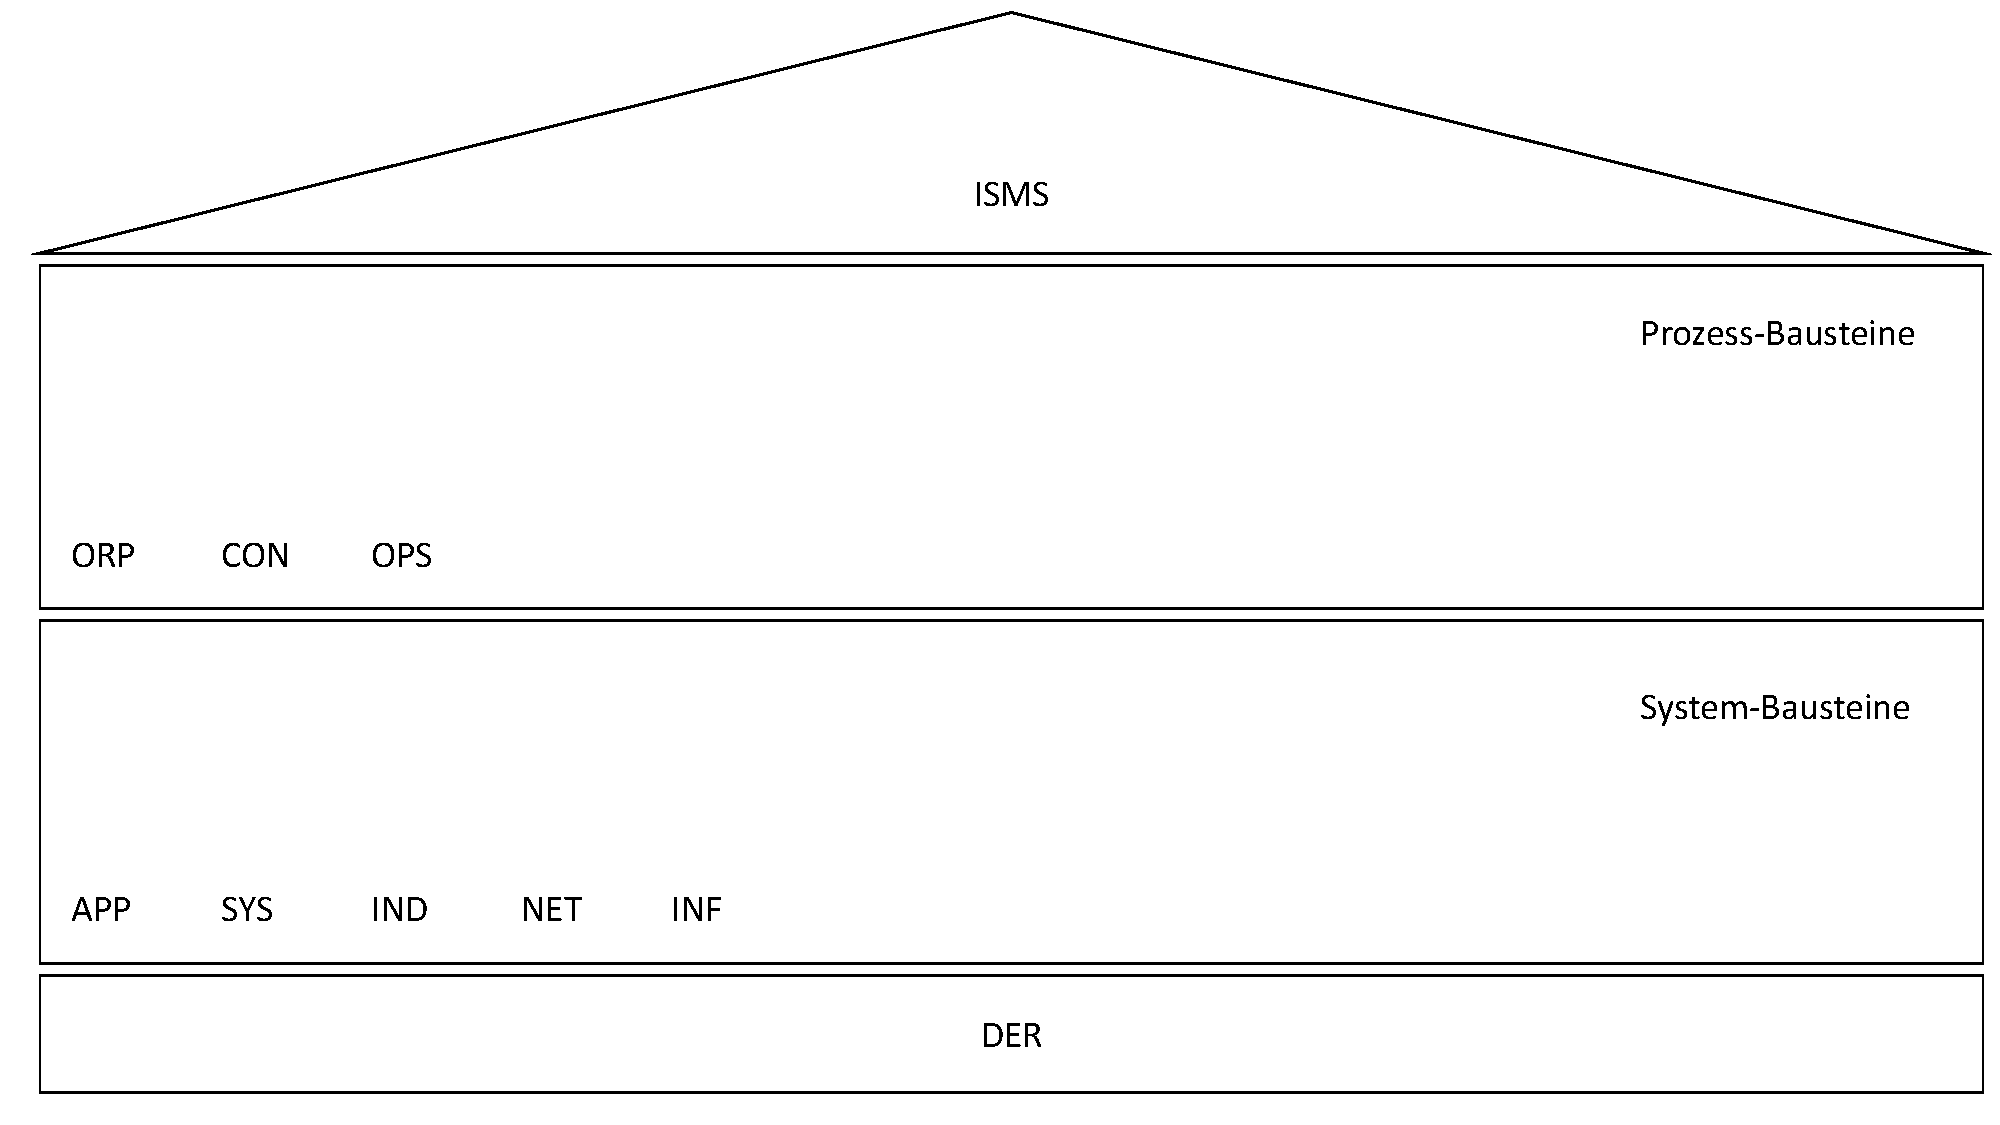
\includegraphics[scale=0.45]{img/bsiSchichtenmodell.pdf}
	\caption{Das Schichtenmodell des IT-Grundschutzes}
	{\footnotesize Quelle: in Anlehnung an \cite[][S.9]{bundesamt_fur_sicherheit_in_der_informationstechnik_bsi_it-grundschutz-kompendium_2020}}
	\label{abb:BSISchichtenmodell}
	%		{\scriptsize \textit{Alle Rechte, einschließlich der Vervielfältigung, Veröffentlichung, Bearbeitung und Übersetzung bleiben der SV Informatik GmbH vorbehalten.}}
\end{figure}

\enquote{Die Prozessbausteine, die in der Regel für sämtliche oder große Teile eines Informationsverbunds gleichermaßen
gelten, unterteilen sich in die folgenden Schichten, die wiederum aus weiteren Teilschichten bestehen können.
\begin{itemize}
	\item Die Schicht ISMS enthält als Grundlage für alle weiteren Aktivitäten im Sicherheitsprozess den Baustein Sicherheitsmanagement.
	\item Die Schicht ORP befasst sich mit organisatorischen und personellen Sicherheitsaspekten. In diese Schicht fallen beispielsweise die Bausteine Organisation und Personal.
	\item Die Schicht CON enthält Bausteine, die sich mit Konzepten und Vorgehensweisen befassen. Typische Bausteine
	der Schicht CON sind unter anderem Kryptokonzept und Datenschutz.
	\item Die Schicht OPS umfasst alle Sicherheitsaspekte betrieblicher Art. Insbesondere sind dies die Sicherheitsaspekte des operativen IT-Betriebs, sowohl bei einem Betrieb im Haus, als auch bei einem IT-Betrieb, der in Teilen oder komplett durch Dritte betrieben wird. Ebenso enthält er die Sicherheitsaspekte, die bei einem IT-Betrieb für Dritte zu beachten sind. Beispiele für die Schicht OPS sind die Bausteine Schutz vor Schadprogrammen und Outsourcing für Kunden.
	\item In der Schicht DER finden sich alle Bausteine, die für die Überprüfung der umgesetzten Sicherheitsmaßnahmen, die Detektion von Sicherheitsvorfällen sowie die geeigneten Reaktionen darauf relevant sind. Typische Bausteine der Schicht DER sind Behandlung von Sicherheitsvorfällen und Vorsorge für IT-Forensik.
\end{itemize}
Neben den Prozess-Bausteinen beinhaltet das IT-Grundschutz-Kompendium auch System-Bausteine. Diese werden
in der Regel auf einzelne Zielobjekte oder Gruppen von Zielobjekten angewendet. Die System-Bausteine unterteilen sich in die folgenden Schichten. Ähnlich wie die Prozess-Bausteine können auch die System-Bausteine aus weiteren Teilschichten bestehen.

\begin{itemize}
	\item Die Schicht APP beschäftigt sich mit der Absicherung von Anwendungen und Diensten, unter anderem in den
	Bereichen Kommunikation, Verzeichnisdienste, netzbasierte Dienste sowie Business- und Client-Anwendungen.
	Typische Bausteine der Schicht APP sind Allgemeine Groupware, Office-Produkte, Webserver und Relationale
	Datenbanksysteme.
	\item Die Schicht SYS betrifft die einzelnen IT-Systeme des Informationsverbunds, die ggf. in Gruppen zusammengefasst wurden. Hier werden die Sicherheitsaspekte von Servern, Desktop-Systemen, Mobile Devices und sonstigen IT-Systemen wie Druckern und TK-Anlagen behandelt. Zur Schicht SYS gehören beispielsweise Bausteine zu
	konkreten Betriebssystemen, Allgemeine Smartphones und Tablets sowie Drucker, Kopierer und Multifunktionsgeräte.
	\item Die Schicht IND befasst sich mit Sicherheitsaspekten industrieller IT. In diese Schicht fallen beispielsweise die Bausteine Betriebs- und Steuerungstechnik, Allgemeine ICS-Komponente und Speicherprogrammierbare Steuerung (SPS).
	\item Die Schicht NET betrachtet die Vernetzungsaspekte, die sich nicht primär auf bestimmte IT-Systeme, sondern
	auf die Netzverbindungen und die Kommunikation beziehen. Dazu gehören zum Beispiel die Bausteine NetzManagement, Firewall und WLAN-Betrieb.
	\item Die Schicht INF befasst sich mit den baulich-technischen Gegebenheiten, hier werden Aspekte der infrastrukturellen Sicherheit zusammengeführt. Dies betrifft unter anderem die Bausteine Allgemeines Gebäude und Rechenzentrum.
\end{itemize}}\autocite[][S.23-24]{bundesamt_fur_sicherheit_in_der_informationstechnik_bsi_it-grundschutz-kompendium_2020}




% Ehrenwörtliche Erklärung ewerkl.tex einziehen
% !TEX root =  master.tex

\clearpage
\chapter*{Ehrenwörtliche Erklärung}

% Wird die folgende Zeile auskommentiert, erscheint die ehrenwörtliche
% Erklärung im Inhaltsverzeichnis.
\addcontentsline{toc}{chapter}{Ehrenwörtliche Erklärung}

Ich versichere hiermit, dass ich die vorliegende Arbeit mit dem Thema: \textit{\DerTitelDerArbeit} selbstständig verfasst und keine anderen als die angegebenen Quellen und Hilfsmittel benutzt habe. Ich versichere zudem, dass die eingereichte elektronische Fassung mit der gedruckten Fassung übereinstimmt.

%\vspace{3cm}
%\noindent\rule{5cm}{.4pt}\hfill\rule{5cm}{.4pt}\par
%Ort, Datum \hfill \DerAutorDerArbeit

\vspace{3cm}
\noindent Mannheim, 08.05.2020 \hfill\rule{5cm}{.4pt}\par
\noindent\hfill \DerAutorDerArbeit



\end{document}
